\documentclass[rs,english,toc,lot,lof,index,wide,overfull]{prismdoc}
%=====================================
% PRISMDOC: Start Dokument Information
%=====================================
%\usepackage{longtable}
\usepackage{natbib}
\usepackage{verbatim}
\usepackage{epsfig}
\usepackage{rotating}
\usepackage{graphicx}
\usepackage{amssymb}
%
% Specifications for cover pages: 
%
\prismdocNum{}
\prismdocTitel{{\fontsize{13}{16}\selectfont
    OASIS3 User Guide \\ [0.5ex]
    \it{oasis3\_3 }}}
\prismdocAutor{Edited by:  \\ [0.5ex]
            S. Valcke, CERFACS/CNRS URA No1875 \\[0.5ex]
}
\prismdocVersion{CERFACS TR/CMGC/XX/XX}
\prismdocFName{Sophie Valcke}
\prismdocFAff{CERFACS}
%\prismdocFEM{toto}
\prismdocFEm{oasishelp(at)cerfacs.fr} 
%\prismdocSName{Ren\'e Redler}
\prismdocFPhone{+33-5-61-19-30-76}
%\prismdocSPhone{+49-2241-92-52-40}
%\prismdocFWp{wpnn}
%\prismdocSWp{wpnn}
\prismdocDate{May 2010}


%====================================
% PRISMDOC: End Dokument Information
%====================================
\newcommand{\antispace}{\vspace*{-2ex}}
\newcommand{\bigspace}{\vspace*{+4ex}}
\newcommand{\medspace}{\vspace*{+2ex}}
\newcommand{\smallspace}{\vspace*{+0ex}}
\newcommand{\marginlabel}[1]{\mbox{}\marginpar{\raggedleft\hspace{0pt}#1}}
\newcommand{\imprt}{\marginlabel{{\bfseries\Huge !}}}
\newcommand{\imprtbig}{\marginlabel{{\bfseries\Huge !}}}
\newcommand{\bignote}{\marginlabel{{\bfseries\Huge !!!}}}
\newcommand{\imprtsm}{\marginlabel{{\bfseries\LARGE !}}}
\newcommand{\imnote}{\marginlabel{{\bfseries\LARGE !!!}}}
\newcommand{\bcntr}{\begin{center}}
\newcommand{\ecntr}{\end{center}}

%\includeonly{documentation}
\begin{document}
\prismdocHeader

\include{defines}
\newpage
%%
%\addcontentsline{toc}{section}{Acknowledgements}
%\centerline{\bf Acknowledgements}
.

\vspace{3cm}

{\bf ACKNOWLEDGMENTS}
 
\vspace{1.5cm}
 We would like to thank the main past or present developers of OASIS
are (in alphabetical order, with the name of their institution at the time of their contribution to OASIS):

Arnaud Caubel (LSCE/IPSL \& FECIT/Fujitsu),
Damien Declat (CERFACS),
Italo Epicoco (CMCC),
Veronika Gayler (MPI-M\&D),
Josefine Ghattas (CERFACS),
Jean Latour (CERFACS \& Fujitsu-Fecit),
Eric Maisonnave (CERFACS),
Silvia Mocavero (CMCC),
Elodie Rapaport (CERFACS),
Hubert Ritzdorf (CCRLE-NEC),
Sami Saarinen (ECMWF),
Eric Sevault (M\'et\'eo-France),
Laurent Terray (CERFACS),
Olivier Thual (CERFACS),
Reiner Vogelsang (SGI Germany),
Li Yan (CERFACS).

\vspace{0.5cm}
We also would like to thank the following people for their help
and suggestions in the design of the OASIS software (in alphabetical
order, with the name of their institution at the time of their contribution to OASIS):

Dominique Astruc (IMFT),
Chandan Basu (NSC, Sweden),
Sophie Belamari (M\'et\'eo-France),
Dominique Bielli (M\'et\'eo-France),
Gilles Bourhis (IDRIS),
Pascale Braconnot (IPSL/LSCE),
Sandro Calmanti (M\'et\'eo-France),
Christophe Cassou (CERFACS),
Yves Chartier (RPN),
Jalel Chergui (IDRIS),
Philippe Courtier (M\'et\'eo-France),
Philippe Dandin (M\'et\'eo-France),
Michel D\'equ\'e (M\'et\'eo-France),
Ralph Doescher (SMHI),
Jean-Louis Dufresne (LMD),
Jean-Marie Epitalon (CERFACS),
Laurent Fairhead (LMD),
Uwe Fladrich (SMHI),
Marie-Alice Foujols (IPSL),
Gilles Garric (CERFACS),
Eric Guilyardi (CERFACS),
Charles Henriet (CRAY France),
Pierre Herchuelz (ACCRI),
Maurice Imbard (M\'et\'eo-France),
Luis Kornblueh (MPI-M),
Stephanie Legutke (MPI-M\&D),
Claire L\'evy (LODYC),
Olivier Marti (IPSL/LSCE),
S\'ebastien Masson (IPSL/LOCEAN)
Claude Mercier (IDRIS),
Pascale Noyret (EDF),
Andrea Piacentini (CERFACS),
Marc Pontaud (M\'et\'eo-France),
Adam Ralph (ICHEC),
Ren\'e Redler (MPI-M),
Tim Stockdale (ECMWF),
Rowan Sutton (UGAMP),
V\'eronique Taverne (CERFACS),
Jean-Christophe Thil (UKMO),
Nils Wedi (ECMWF).




\newpage
\chapter{Introduction}
\label{sec_step}

In 1991, CERFACS started the development of
a software interface to couple existing ocean and atmosphere numerical General
Circulation Models. Today, different versions of the 
OASIS coupler are used by about 45 modelling groups all around the
world on different computing platforms \citep{valcke8}\footnote{A list of
coupled models realized with OASIS can be found at https://verc.enes.org/oasis/oasis-dedicated-user-support-1/some-current-users}.
OASIS sustained development is ensured by a collaboration
between CERFACS and the Centre National de la Recherche Scientifique
(CNRS) and its maintainance and user support is presently reinforced
with additional resources coming from the IS-ENES2 European project (\# 312979).

The current OASIS3-MCT internally uses MCT, the Model
Coupling Toolkit\footnote{www.mcs.anl.gov/research/projects/mct/} \citep{mct_larson} \newline \citep{mct_jacob}, developed by the Argonne National Laboratory in the USA. MCT implements fully parallel regridding, as a parallel matrix vector 
multiplication, and parallel distributed exchanges of the coupling
fields, based on pre-computed regridding weights and addresses. 
Its design philosophy, based on flexibility and minimal invasiveness,
is close to the OASIS approach. 
MCT has proven parallel performance and is, most notably, the
underlying coupling software used in National Center for Atmospheric
Research Community Earth System Model (NCAR CESM).

OASIS3-MCT is a portable set of Fortran 77, Fortran 90 and C
routines. Low-intrusiveness, portability and flexibility are
OASIS3-MCT key design concepts. After compilation OASIS3-MCT is a
coupling library to be linked to the component models, and which main
function is to interpolate and exchange the coupling fields between
them to form a coupled system.  OASIS3-MCT supports  coupling of 2D
logically-rectangular fields but 3D fields and 1D fields expressed on
unstructured grids are also supported using a one dimension
degeneration of the structures. Thanks to MCT, all transformations,
including regridding, are performed in parallel on the set of source or
target component processes and all coupling echanges are now executed
in parallel directly between the component processes via Message Passing Interface
(MPI). OASIS3-MCT also supports file I/O using netcdf. 

The new version, OASIS3-MCT\_3.0 supports coupling exchanges between
components deployed in much more diverse configurations than
before. It is of course possible to implement coupling exchanges
between two components corresponding to two different executables
running concurrently on separate sets of tasks, as before, but also
between two components running concurrently on separate sets of tasks
within one same executable, or between different
sub-components defined on separate or overlapping sets of tasks within
one executable. It is also now possible to
have some or all tasks of a component not participating to the
coupling exchanges. 

In spite of the significant changes in underlying implementation,
usage of OASIS3-MCT in the codes has largely remained unchanged with
respect to previous OASIS3 versions.
To communicate with another component, or to perform I/O actions, a
component model needs to include few specific calls of the Application Programmig Interface (API)  OASIS3-MCT coupling library.  The {\it namcouple} configuration file is also largely unchanged
relative to OASIS3, although several options are either deprecated, not used
or not supported. 

A Graphical User Interface is now available to build
the {\it namcouple} configuration file for one's specific coupled
system. The OASIS3-MCT GUI is an application of OPENTEA, a graphical
interface used by different codes and developed at CERFACS. The
sources of the GUI are located in the {\tt oasis3-mct/util/oasisgui}
directory; a short description of the OASIS GUI is given in the README
file therein and the GUI itself includes all relevant explanations on-line.

The changes between previous versions and the
current one are listed in appendix \ref{sec_changes}.
 
First tests done with up to
16000 cores on the Bullx Curie machine at the {\it Tr\`es Grand Centre de
Calcul} near Paris are very encouraging
and it is therefore very likely that OASIS3-MCT will provide an efficient and
easy-to-use coupling solution for many climate modelling groups in the few years to come. 

%See appendix \ref{sec_changes} for a more detailed list of changes in this %version.

\section{Step-by-step use of OASIS3-MCT}

To use OASIS3-MCT for coupling models (and/or perform I/O
actions), one has to follow these steps:
\begin{enumerate}
\item Obtain OASIS3-MCT source code (see chapter \ref{sec_Obtaining}).
\item Get familiar with OASIS3-MCT by going through the tutorial steps. The tutorial sources are given in directory {\tt
  examples/tutorial} and all explanations are provided in the document
{\tt tutorial.pdf} therein. The tutorial also helps one to
practice with the Graphical User Interface.

\item Identify the coupling or I/O fields and adapt the codes to
  implement the coupling exchanges with the OASIS3-MCT coupling library based on MPI message passing.
  The OASIS3-MCT coupling library uses NetCDF and therefore can also be used to perform I/O actions
  from/to disk files.  For more detail on how to use the 
  OASIS3-MCT API in the codes, see chapter \ref{sec_modelinterfacing}.

\item Define all coupling and I/O parameters and the transformations
  required to adapt each coupling field from the source model grid to
  the target model grid; on this basis, prepare OASIS3-MCT configuring file 
  {\it namcouple} preferably using the
  Graphical User Interface  (see chapter \ref{sec_namcouple}). 
  OASIS3-MCT supports different interpolation algorithms as described in
  chapter \ref{sec_transformations}.  Regridding files can be computed
  online using the SCRIP options, or offline and read in during the run using the MAPPING
  transformation.

{\bf We strongly recommend to tests off-line the quality of the chosen transformations and regriddings} using the environment available in {\tt
  examples/test\_interpolation} and explanations provided in the document {\tt test\_interpolation.pdf} therein. 

\item Generate required auxiliary data files (see chapter
  \ref{sec_auxiliary}).
\item Compile OASIS3-MCT, the component models and start the coupled
  experiment. Details on how to compile and run a coupled model with OASIS3-MCT can be found in section \ref{sec_compilationrunning}. 

\end{enumerate}

If you need extra help, do not hesitate to contact us (see contact
details on the back of the cover page).

\section{OASIS3-MCT sources}
\label{sec_Obtaining}
OASIS3-MCT sources are available from CERFACS SVN server. To obtain more detail on downloading
the sources, please fill in the registration form at
https://verc.enes.org/oasis/download/oasis-registration-form .

OASIS3-MCT directory structure is the following one:

\begin{verbatim}
 - oasis3-mct/lib/psmile         OASIS3-MCT coupling library
                 /scrip          SCRIP interpolation library
                 /mct            Model Coupling Toolkit Coupling Software
                  
 - oasis3-mct/doc                OASIS3-MCT User Guide

 - oasis3-mct/util/make_dir      Utilities to compile OASIS3-MCT
                  /oasisgui      Graphical User Interface to the
                                 namcouple configuration file
                  /lucia         Tool for load balancing analysis (XXX)

 - oasis3-mct/examples           Environment to compile, run and use
                                 different toy coupled models. 
\end{verbatim}
\newpage
\section{Licenss and Copyrights}
 
\subsection{OASIS3-MCT license and copyright statement}

Copyright © 2015 Centre Europ\'een de Recherche et Formation
Avanc\'ee en Calcul Scientifique (CERFACS).  

This software and ancillary information called OASIS3-MCT is free
software.  CERFACS has rights to use, reproduce, and distribute
OASIS3-MCT. The public may copy, distribute, use, prepare derivative works and
publicly display OASIS3-MCT under the terms of the Lesser GNU General
Public License (LGPL) as published by the Free Software Foundation,
provided that this notice and any statement of authorship are
reproduced on all copies. If OASIS3-MCT is modified to produce derivative
works, such modified software should be clearly marked, so as not to
confuse it with the OASIS3-MCT version available from CERFACS.

The developers of the OASIS3-MCT software are researchers attempting to
build a modular and user-friendly coupler accessible to the climate
modelling community. Although we use the tool ourselves and have made
every effort to ensure its accuracy, we can not make any
guarantees. We provide the software to you for free. In return,
you --the user-- assume full responsibility for use of the software. The
OASIS3-MCT software comes without any warranties (implied or expressed) and
is not guaranteed to work for you or on your computer. Specifically,
CERFACS and the various individuals involved in development and
maintenance of the OASIS3-MCT software are not responsible for any damage
that may result from correct or incorrect use of this software.

\subsection{MCT copyright statement}
\label{sec_MCT}

                            Modeling Coupling Toolkit (MCT) Software

Copyright © 2011, UChicago Argonne, LLC as Operator of Argonne National Laboratory. All rights reserved.

Redistribution and use in source and binary forms, with or without modification, are permitted provided that the following conditions are met:
\begin{enumerate}
\item Redistributions of source code must retain the above copyright notice, this list of conditions and the following disclaimer.
\item Redistributions in binary form must reproduce the above copyright notice, this list of conditions and the following disclaimer in the documentation and/or other materials provided with the distribution.
\item The end-user documentation included with the redistribution, if any, must include the following acknowledgment: "This product includes software developed by the UChicago Argonne, LLC, as Operator of Argonne National Laboratory." Alternately, this acknowledgment may appear in the software itself, if and wherever such third-party acknowledgments normally appear.

This software was authored by:
\begin{itemize}
\item Argonne National Laboratory Climate Modeling Group, Mathematics and Computer Science Division, Argonne National Laboratory, Argonne IL 60439
\item Robert Jacob, tel: (630) 252-2983, E-mail: jacob@mcs.anl.gov
\item Jay Larson, E-mail: larson@mcs.anl.gov
\item Everest Ong
\item Ray Loy
\end{itemize}

\item WARRANTY DISCLAIMER. THE SOFTWARE IS SUPPLIED "AS IS" WITHOUT WARRANTY OF ANY KIND. THE COPYRIGHT HOLDER, THE UNITED STATES, THE UNITED STATES DEPARTMENT OF ENERGY, AND THEIR EMPLOYEES: (1) DISCLAIM ANY WARRANTIES, EXPRESS OR IMPLIED, INCLUDING BUT NOT LIMITED TO ANY IMPLIED WARRANTIES OF MERCHANTABILITY, FITNESS FOR A PARTICULAR PURPOSE, TITLE OR NON-IN- FRINGEMENT, (2) DO NOT ASSUME ANY LEGAL LIABILITY OR RESPONSIBILITY FOR THE ACCURACY, COMPLETENESS, OR USEFULNESS OF THE SOFTWARE, (3) DO NOT REPRESENT THAT USE OF THE SOFTWARE WOULD NOT INFRINGE PRIVATELY OWNED RIGHTS, (4) DO NOT WARRANT THAT THE SOFTWARE WILL FUNCTION UNINTERRUPTED, THAT IT IS ERROR-FREE OR THAT ANY ERRORS WILL BE CORRECTED. 

\item LIMITATION OF LIABILITY. IN NO EVENT WILL THE COPYRIGHT HOLDER, THE UNITED STATES, THE UNITED STATES DEPARTMENT OF ENERGY, OR THEIR EMPLOYEES: BE LIABLE FOR ANY INDIRECT, INCIDENTAL, CONSEQUENTIAL, SPECIAL OR PUNITIVE DAMAGES OF ANY KIND OR NATURE, INCLUDING BUT NOT LIMITED TO LOSS OF PROFITS OR LOSS OF DATA, FOR ANY REASON WHATSOEVER, WHETHER SUCH LIABILITY IS ASSERTED ON THE BASIS OF CONTRACT, TORT (INCLUDING NEGLIGENCE OR STRICT LIABILITY), OR OTHERWISE, EVEN IF ANY OF SAID PARTIES HAS BEEN WARNED OF THE POSSIBILITY OF SUCH LOSS OR DAMAGES.

\end{enumerate}

\subsection{The SCRIP 1.4 license copyright statement}
\label{sec_SCRIP}

The SCRIP 1.4 copyright statement reads as follows:

``Copyright © 1997, 1998 the Regents of the University of California.
This software and ancillary information (herein called SOFTWARE)
called SCRIP is made available under the terms described here. The
SOFTWARE has been approved for release with associated LA-CC Number
98-45. Unless otherwise indicated, this SOFTWARE has been authored by
an employee or employees of the University of California, operator of
Los Alamos National Laboratory under Contract No. W-7405-ENG-36 with
the United States Department of Energy. The United States Government
has rights to use, reproduce, and distribute this SOFTWARE. The public
may copy, distribute, prepare derivative works and publicly display
this SOFTWARE without charge, provided that this Notice and any
statement of authorship are reproduced on all copies. Neither the
Government nor the University makes any warranty, express or implied,
or assumes any liability or responsibility for the use of this
SOFTWARE. If SOFTWARE is modified to produce derivative works, such
modified SOFTWARE should be clearly marked, so as not to confuse it
with the version available from Los Alamos National Laboratory.''

\newpage
\chapter{OASIS3 sources, license and Copyright}
\label{sec_Obtaining}
%               ----------------------------------
%
%
\section{OASIS3 sources}
OASIS3 sources, related libraries, and TOYOASIS3
coupled model sources and data are available from CERFACS SVN server. To obtain more detail on how to download
the sources, please
contact us (see contact details on the back of the cover page).

OASIS3 directory structure is the following one:

\begin{verbatim}

 - oasis3/lib/psmile      PRISM System Model Interface Library
             /scrip       SCRIPR interpolation library
             /mct         Model Coupling Toolkit Coupling Software
                  
 - oasis3/doc             OASIS3 documentation
 
 - oasis3/util/make_dir   Utilities to compile OASIS3 (see section 8.1) 

 - oasis3/examples/tutorial  environment to run the tutorial toymodel
                              (see section 8.3)
 
\end{verbatim}
%                              
% 
%                  /sxgmem/    GMEM communication library
%
%\end{verbatim}

\section{License and Copyright}

\subsection{OASIS3 license and copyright statement}

Copyright © 2010 Centre Europeen de Recherche et Formation
Avancee en Calcul Scientifique (CERFACS).  

This software and ancillary information called OASIS3 is free
software.  CERFACS has rights to use, reproduce, and distribute
OASIS3. The public may copy, distribute, use, prepare derivative works and
publicly display OASIS3 under the terms of the Lesser GNU General
Public License (LGPL) as published by the Free Software Foundation,
provided that this notice and any statement of authorship are
reproduced on all copies. If OASIS3 is modified to produce derivative
works, such modified software should be clearly marked, so as not to
confuse it with the OASIS3 version available from CERFACS.

The developers of the OASIS3 software are researchers attempting to
build a modular and user-friendly coupler accessible to the climate
modelling community. Although we use the tool ourselves and have made
every effort to ensure its accuracy, we can not make any
guarantees. We provide the software to you for free. In return,
you--the user--assume full responsibility for use of the software. The
OASIS3 software comes without any warranties (implied or expressed) and
is not guaranteed to work for you or on your computer. Specifically,
CERFACS and the various individuals involved in development and
maintenance of the OASIS3 software are not responsible for any damage
that may result from correct or incorrect use of this software.

\subsection{The SCRIP 1.4 license copyright statement}
\label{sec_SCRIP}

The SCRIP 1.4 copyright statement reads as follows:

 ``Copyright © 1997, 1998 the Regents of the
University of California.  This software and ancillary information
(herein called SOFTWARE) called SCRIP is made available under the
terms described here. The SOFTWARE has been approved for release with
associated LA-CC Number 98-45. Unless otherwise indicated, this
SOFTWARE has been authored by an employee or employees of the
University of California, operator of Los Alamos National Laboratory
under Contract No. W-7405-ENG-36 with the United States Department of
Energy. The United States Government has rights to use, reproduce, and
distribute this SOFTWARE. The public may copy, distribute, prepare
derivative works and publicly display this SOFTWARE without charge,
provided that this Notice and any statement of authorship are
reproduced on all copies. Neither the Government nor the University
makes any warranty, express or implied, or assumes any liability or
responsibility for the use of this SOFTWARE. If SOFTWARE is modified
to produce derivative works, such modified SOFTWARE should be clearly
marked, so as not to confuse it with the version available from Los
Alamos National Laboratory.''

\newpage
\chapter{Interfacing a component code with OASIS3-MCT}
\label{sec_modelinterfacing}

At run-time, OASIS3-MCT performs parallel exchange of coupling data between parallel
components and sub-components and allows remapping (interpolation), time integration or accumulation and other transformations of these coupling fields. 

This chapter describes how to adapt the component codes to couple them through OASIS3-MCT. 

OASIS3-MCT supports coupling exchanges between parallel
components and sub-components deployed in diverse
configurations; the different possibilities and how to use
the OASIS3-MCT library accordingly are described in section
\ref{sec_deploy}. 
The OASIS3-MCT Application Programming Interface (API) includes different classes of modules or routines that are described in details in section \ref{API}.
Finally, in section \ref{subsubsec_Algoritms}, different coupling
algorithms are illustrated and details on how to reproduce them with
OASIS3-MCT are provided, together with more information on the {\tt LAG} and {\tt
  SEQ} indices.

\section{Configurations of components supported}
\label{sec_deploy}

Since OASIS3-MCT\_3.0, coupling exchanges between components and
sub-components deployed in a much larger diversity of configurations
are now supported. This is illustrated on figure
\ref{Fig_coupling_layouts_a} and how to use the OASIS3-MCT library
accordingly is detailed on figure \ref{Fig_coupling_layouts_b}. All
OASIS3-MCT API routines are also described in details in section
\ref{API}. 

We call here an ``executable'' a compiled code
  forming a part of or the whole coupled system (started with the
  mpirun or mpiexec command). A ``component'' is the ensemble of
  processes, or tasks, within the coupled system calling {\tt oasis\_init\_comp}
  with the same {\tt comp\_name} argument (see section
  \ref{init_comp}). A ``sub-component'' is the subset of tasks within a
  component sending or receiving coupling fields on a specific grid;
  of course, a component may have only one sub-component
  that gathers all its tasks.

Practical examples of how to use the OASIS3-MCT library are also given in {\tt examples/} {\tt tutorial} and {\tt examples/test\_1bin\_ocnice} (see sections \ref{subsec_tutorial} and \ref{subsec_1bin_ocnice}). 

Since OASIS3-MCT\_3.0, it is possible to (the text between [ and ] refers to figure \ref{Fig_coupling_layouts_a}) :

\begin{figure}
  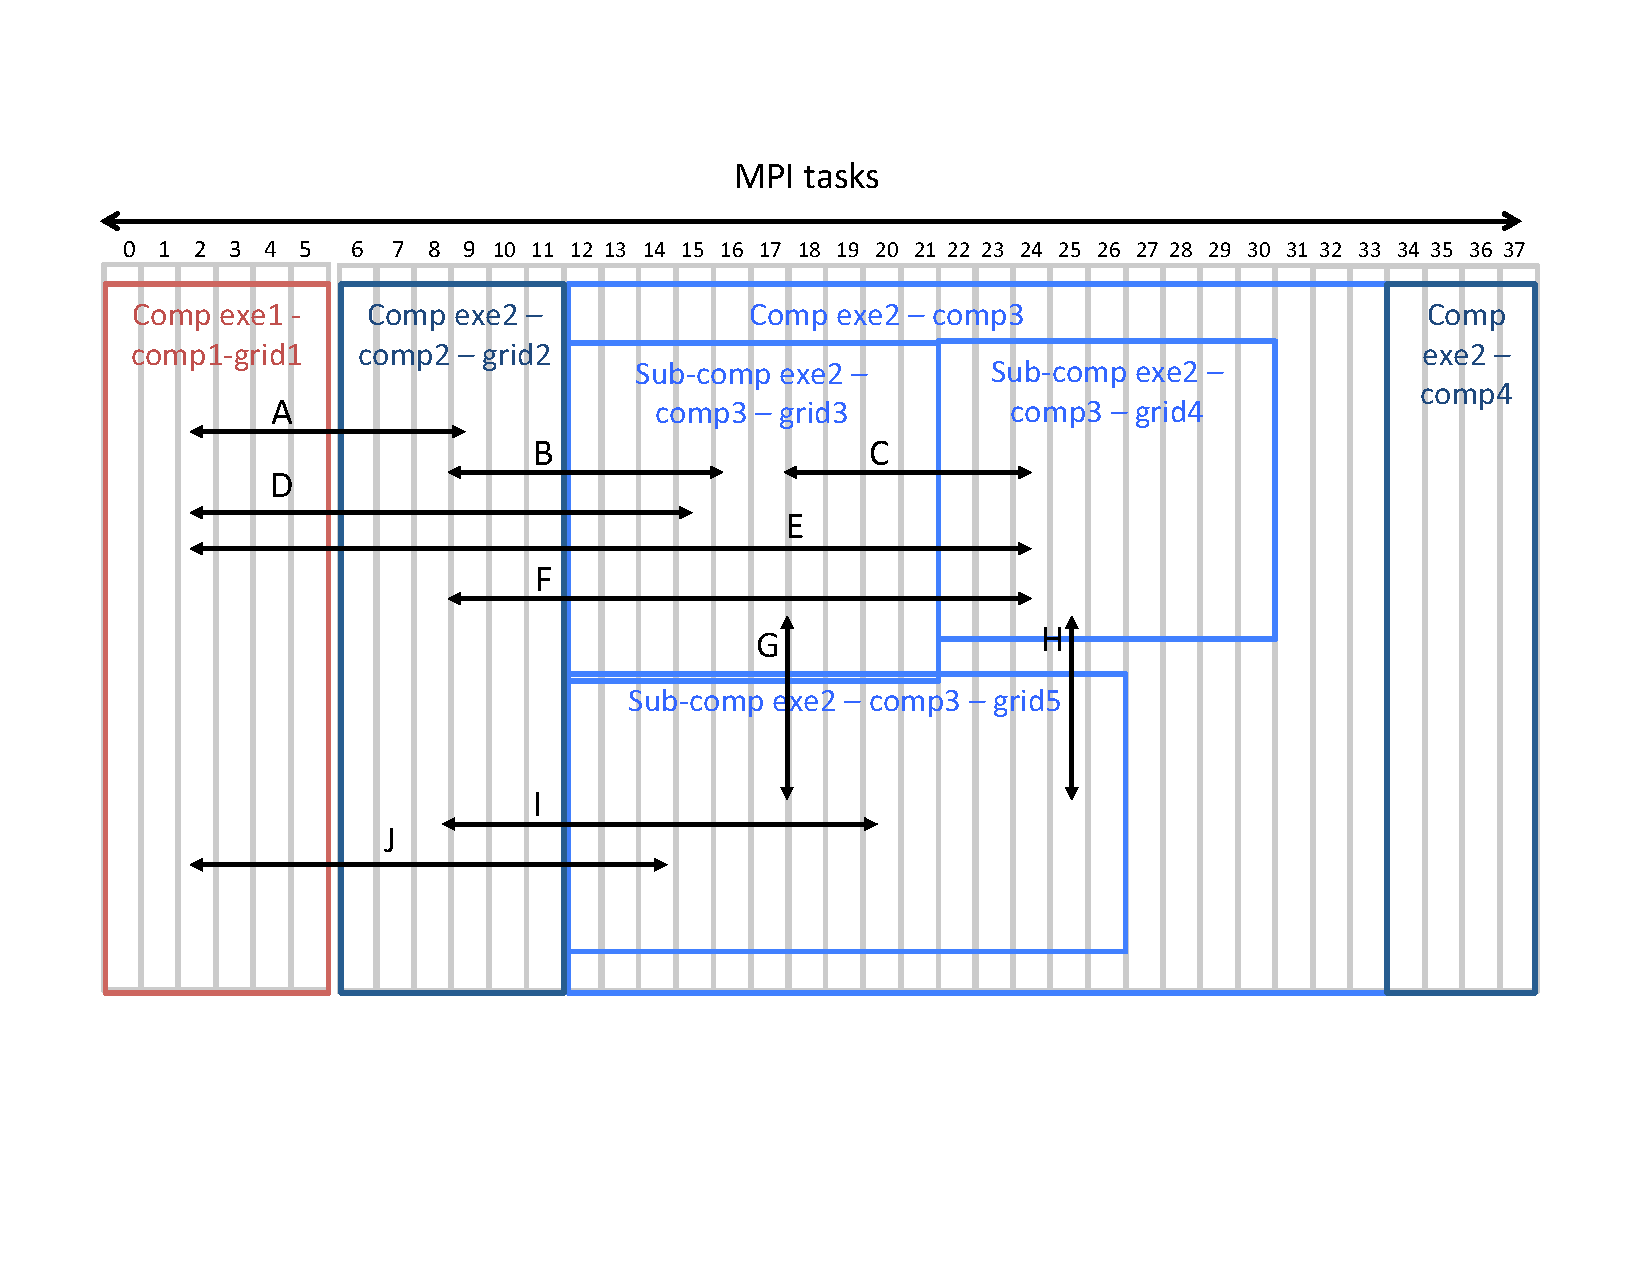
\includegraphics[scale=.6]{figures/coupling_layouts_a}
  \caption{The different configuration of components supported by OASIS3-MCT\_3.0. Two executables {\tt exe1} and {\tt exe2} are running concurrently on separate sets of MPI tasks (0-5 for {\tt exe1} and 6-37 for {\tt exe2}). Executable {\tt exe1} includes only one component {\tt comp1} that has coupling fields defined on only one grid {\tt grid1} (decomposed on all its 6 tasks). Executable {\tt exe2} includes 3 components, {\tt comp2}, {\tt comp3}, and {\tt comp4} running concurrently respectively on tasks 6-11, 12-33 and 34-37. Component {\tt comp2} participates in the coupling with fields defined on only one coupling grid {\tt grid2} (decomposed on all its 5 tasks) while {\tt comp4} does not participate at all in the coupling. 
Component {\tt comp3} has 3 sub-components, respectively exchanging
coupling fields defined on {\tt grid3} (tasks 12-21), {\tt grid4}
(tasks 22-30) and {\tt grid5} (tasks 12-26, therefore overlaping with both {\tt
  grid3} and {\tt grid4}); finally, {\tt comp3} has 3 tasks (31-33)
not involved in the coupling. Sub-components exe2-comp3-grid3 and
exe2-comp3-grid5, or sub-components exe2-comp3-grid4 and
exe2-comp3-grid5 are examples of coupling between sub-components running sequentially on overlapping sets of tasks.}
  \label{Fig_coupling_layouts_a}
\end{figure}

\begin{figure}
  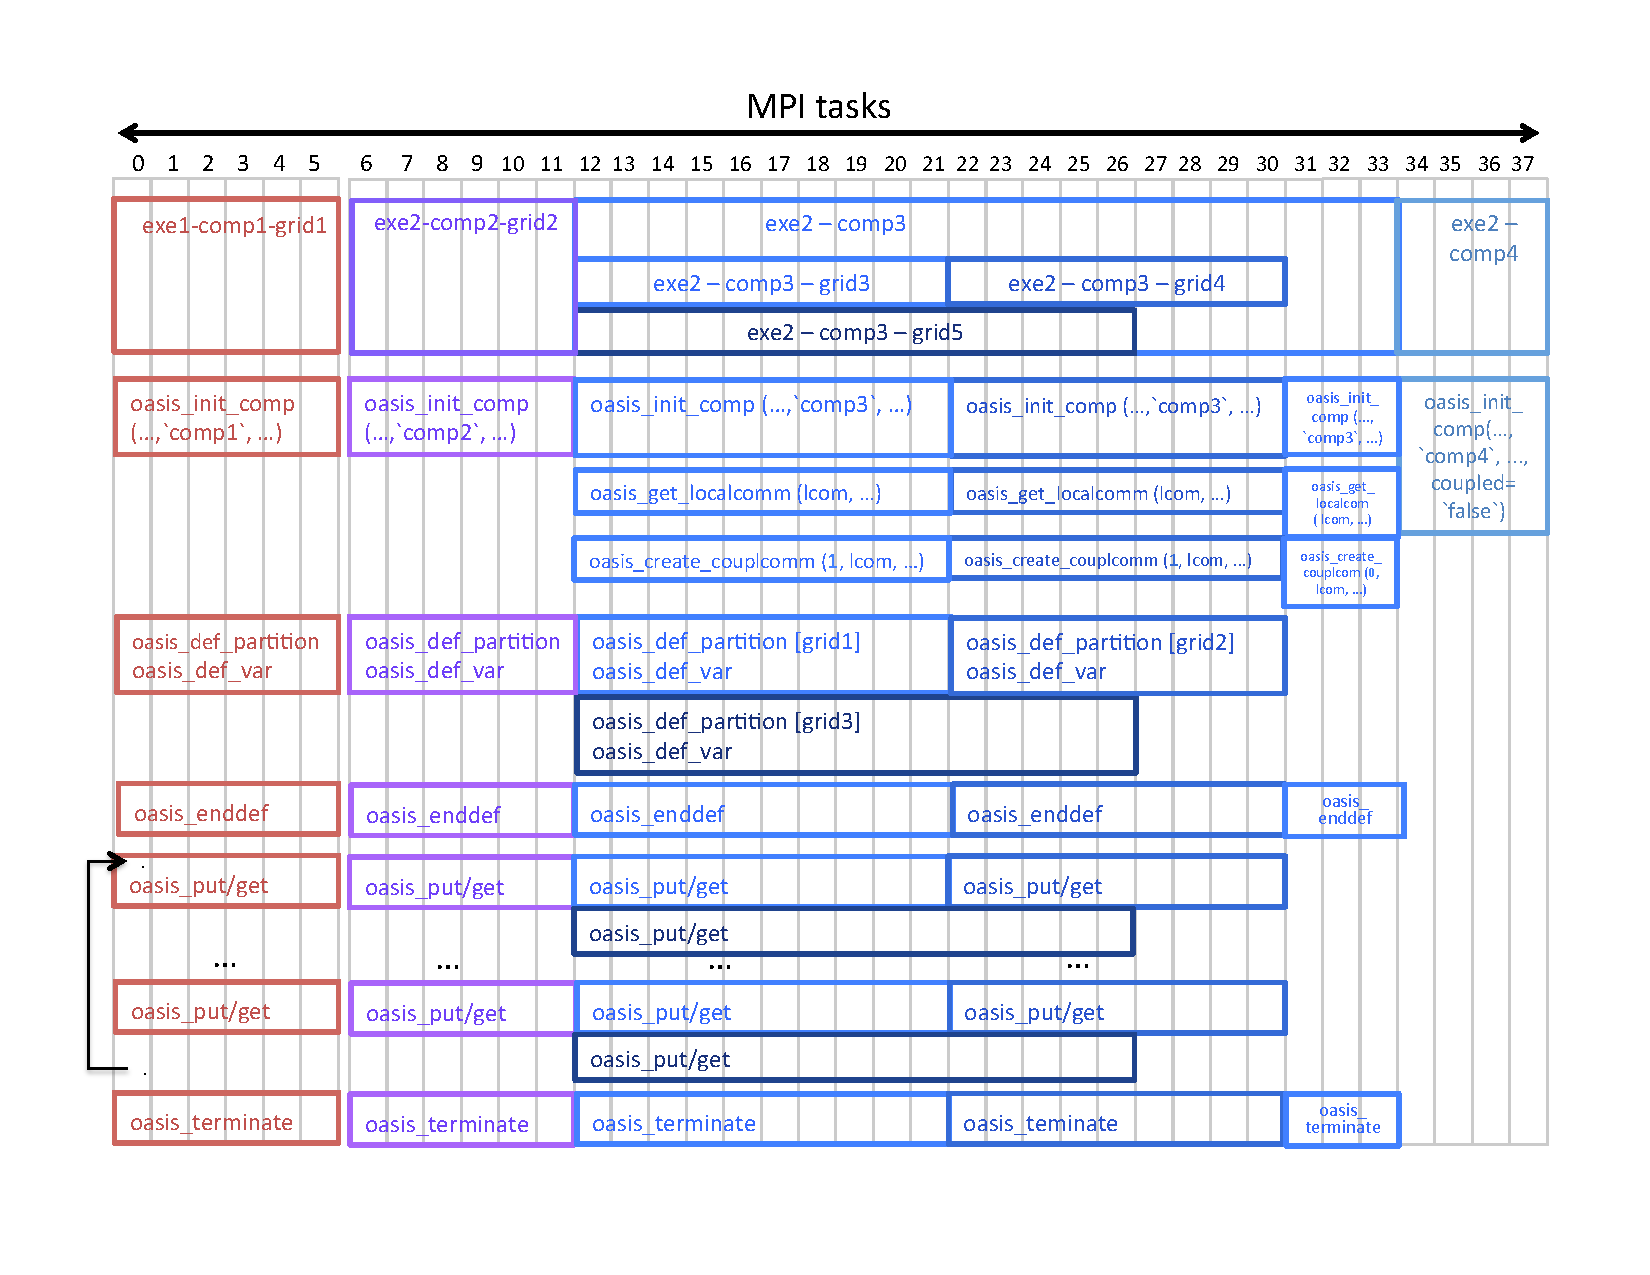
\includegraphics[scale=.6]{figures/coupling_layouts_b}
  \caption{The sequence of OASIS3-MCT calls that have to be implemented in the codes so to allow the configuration of components described on figure \ref{Fig_coupling_layouts_a}.
Each MPI tasks has to call {\tt oasis\_init\_comp} once with the name
of its component as $2^{nd}$ argument. As none of {\tt comp4} tasks is
participating to the coupling, {\tt comp4} tasks calls {\tt
  oasis\_init\_comp} with {\tt coupled=.false.”} as $4^{th}$ argument
and does not call any other OASIS3-MCT routine. As some of {\tt comp3}
tasks are participating to the coupling, all {\tt comp3} tasks have to
call {\tt oasis\_init\_comp}, {\tt oasis\_get\_localcomm}, {\tt
  oasis\_create\_couplcomm}, {\tt oasis\_enddef} and {\tt
  oasis\_terminate} (these are the only routine to be called by {\tt
  comp3} tasks 31-33 not participating to the coupling). To initialise
the coupling exchanges, the tasks of a sub-component holding a field
decomposed on a specific grid have to call the {\tt
  oasis\_def\_partition} to express the decomposition of the grid,
{\tt oasis\_def\_var} to declare the coupling field and {\tt
  oasis\_enddef}. Finally, the tasks of a sub-component exchanging 
coupling fields have to call {\tt oasis\_put} and {\tt oasis\_get} accordingly.
}
  \label{Fig_coupling_layouts_b}
\end{figure}

\begin{itemize}

\item to implement coupling exchanges between two components or
  sub-components running concurrently on separate sets of tasks within two different executables  (as before) [A, D, E, J];
\item to implement coupling exchanges between two components or
  sub-components running concurrently on separate sets of tasks within one same executable [B, F, I];
\item to implement coupling exchanges within one executable between
  two concurrent sub-components [C] 
\item to implement coupling exchanges within one executable between
  two sub-components running sequentially on overlapping sets of tasks (i.e. a task can be coupled to itself calling both the ``put” and the ``get” of the exchange) [G, H]
\item to have some tasks of a component not participating to the coupling exchanges [tasks 31-33 of {\tt exe2-comp3}]
\item to have all processes of a component not participating to the coupling exchanges [{\tt exe2-comp4}, tasks 34-37]

\end{itemize}

The sequence of OASS3-MCT API routines that have to be called in the different cases is detailed on figure  \ref{Fig_coupling_layouts_b}.  These routines are also described in detail in the next section.

\section{OASIS3-MCT Application Programming Interface (API)}
\label{API}

To interact with the rest of the coupled system, few calls of the
OASIS3-MCT library routines, which sources can be found in {\tt
  oasis3-mct/lib/psmile} directory, have to be implemented in the
component codes. They belong to the following classes:
\begin{enumerate}
\item Module to use (section \ref{subsubsec_Use})
\item Initialisation (section \ref{subsubsec_Initialisation})
\item Partition definition (section \ref{subsubsec_Partition})
\item Grid data file definition (section \ref{subsubsec_griddef})
\item Coupling-I/O field declaration (section
  \ref{subsubsec_Declaration})
\item End of definition phase (section
  \ref{subsubsec_Endofdefinition})
\item Coupling-I/O field sending and receiving (section
  \ref{subsubsec_sendingreceiving})
\item Termination (section \ref{subsubsec_Termination})
\item Optional auxiliary routines (section
  \ref{subsubsec_auxroutines})
\end{enumerate}

\subsection{Module to use in the code}
\label{subsubsec_Use}
% {Use}

To use OASIS3-MCT library, a user needs to add in his code:

\begin{itemize}

\item {\tt USE mod\_oasis}

  or

\item {\tt USE mod\_prism}
 
\end{itemize}

Both use statements are valid but only one needs to be used in a particular component. This single use statement provides all methods required. The methods, datatypes, and capabilities
are identical for both the {\tt mod\_prism} or {\tt mod\_oasis}
interfaces, the only difference being the name of the interface. The
interface in module {\tt mod\_prism} is provided for backwards
compatability with prior versions of OASIS3. Use of module {\tt
  mod\_oasis} is recommended and provides access to a set of updated
routine names that will continue to evolve in the future, always
ensuring backward compatibility.  In the following sections, both the
{\tt mod\_prism} and {\tt mod\_oasis} interface names are defined and
a single description of the interface arguments is provided.

\subsection{Initialisation}
\label{subsubsec_Initialisation}
% {Initialisation}

\subsubsection{Coupling initialisation}
\label{init_comp}

\begin{itemize}

\item {\tt CALL oasis\_init\_comp (compid, comp\_name, ierror, coupled, commworld)}
\item {\tt CALL prism\_init\_comp\_proto (compid, comp\_name, ierror, coupled, commworld)}

  \begin{itemize}
  \item {\tt compid [INTEGER; OUT]}: returned component ID
  \item {\tt comp\_name [CHARACTER; IN]}: component name; maximum length of 80 characters 
  \item {\tt ierror [INTEGER; OUT]}: returned error code
  \item {\tt coupled [LOGICAL, OPTIONAL; IN]}: flag to specify if the calling task is participating or not to the coupling ({\tt .true.} by default). 
  \item {\tt commworld [INTEGER, OPTIONAL; IN]} : optional argument to specify the global communicator gathering the components of the coupled model. 
  If not specified, {\tt MPI\_COMM\_WORLD} will be used as the default communicator to startup. All components of the coupled model must 
  specify the same {\tt commworld} argument.

  \end{itemize}
 
  This routine must called by all tasks of all components whether of not they are involved in the coupling \footnote{The component may also call MPI\_Init explicitly, but if so, has to call it before calling {\tt oasis\_init\_comp}; in this case, the component also has to call MPI\_Finalize explicitly, but only after calling {\tt oasis\_terminate}.}. 

A component is defined as the ensemble of tasks  calling {\tt
  oasis\_init\_comp} with the same {\tt comp} {\tt \_name}
argument. If and only if all tasks of a component are excluded from
the coupling, the logical {\tt coupled} can be set to {\tt .false.}
for this component tasks; in this case, {\tt oasis\_init\_comp} is the
only API routine that needs to be called by the component tasks. If at
least one tasks of a component is participating to the coupling, all
component tasks have to call {\tt oasis\_init\_comp} with {\tt
  coupled=.true.} (by default); in this case, the component tasks not
participating to the coupling will also have to call
{\tt oasis\_get\_localcomm}, {\tt oasis\_create\_couplcomm}, {\tt oasis\_enddef} and {\tt oasis\_terminate}.
\end{itemize}

\subsubsection{Communicator for internal parallelisation}
\label{subsec_MPI1}

\begin{itemize}
\item {\tt CALL oasis\_get\_localcomm (local\_comm, ierror )}
\item {\tt CALL prism\_get\_localcomm\_proto (local\_comm, ierror )}

  \begin{itemize}
  \item {\tt local\_comm [INTEGER; OUT]}: value of local communicator
  \item {\tt ierror [INTEGER; OUT]}: returned error code.
  \end{itemize}

  This routine returns the value of a local communicator gathering
  only the tasks of the component, i.e. the tasks that called {\tt
  oasis\_init\_comp} with the same {\tt comp\_name}
argument.

  This may be needed as all executables of the coupled system are started in a pseudo-MPMD
  mode with MPI1 and therefore share automatically the same MPI\_COMM\_WORLD
  communicator.  Another communicator has to be used for the internal
  parallelisation of each component. OASIS3-MCT creates this local
  communicator {\tt local\_comm} based on the value of the {\tt
    comp\_name} argument in the {\tt oasis\_init\_comp} call.

  Retrieving a local communicator {\tt local\_comm} is also needed if
  {\tt oasis\_create\_couplcomm} is called, as {\tt local\_comm} is an argument of this routine (see below).

  % With CLIM-MPI2, OASIS3 executable spawns the component
  % executables at the beginning of the run; the components keep their
  % internal parallelisation context unchanged with respect to their
  % standalone mode. In this case, calling the
  % prism\_get\_localcomm\_proto routine is useless but if called, the
  % communicator MPI\_COMM\_WORLD will be returned as local
  % communicator.
\end{itemize}

\begin{itemize}
\item {\tt CALL oasis\_create\_couplcomm(icpl, local\_comm,
    coupl\_comm, kinfo)}
\item {\tt CALL prism\_create\_couplcomm(icpl, local\_comm,
    coupl\_comm, kinfo)}
  \begin{itemize}
  \item {\tt icpl [INTEGER; IN]}: coupling process flag
  \item {\tt local\_comm [INTEGER; IN]}: MPI communicator with all
    processes of the component
  \item {\tt coupl\_comm [INTEGER; OUT]}: returned MPI communicator
    gathering only component processes participating in the coupling
  \item {\tt kinfo [INTEGER; OUT; OPTIONAL]}: returned error code
  \end{itemize}

  This routine creates a coupling communicator for a subset of
  processes. It is mandatory to call this routine if only a subset of
  the component processes participate in the coupling (e.g. {\tt comp3} in figure
    \ref{Fig_coupling_layouts_b}); in that case, the processes
    involved in the coupling have to call it with icpl=1 while the
    other have to call it with icpl = MPI UNDEFINED. Argument
    local\_comm is the MPI communicator associated with all processes
    of the component returned by oasis\_get\_localcomm. The new coupling 
    communicator is returned in coupl\_comm.

\end{itemize}
If this communicator already exists in the code, the component should
simply provide it to OASIS3-MCT with:

\begin{itemize}
\item {\tt CALL oasis\_set\_couplcomm(coupl\_comm, kinfo)}
\item {\tt CALL prism\_set\_couplcomm(coupl\_comm, kinfo)}
  \begin{itemize}
  \item {\tt coupl\_comm [INTEGER; IN]}: MPI communicator gathering
    only component processes participating in the coupling
  \item {\tt kinfo [INTEGER; OUT; OPTIONAL]}: returned error code
  \end{itemize}

  This routine allows to provide a local coupling communicator to
  OASIS3-MCT, given that it already exists in the code. The value of
  {\tt coupl\_comm} must be the value of this local coupling
  communicator for the processes participating to the coupling and it
  must be {\tt MPI\_COMM\_NULL} for processes not involved in the
  coupling.
\end{itemize}

\subsection{Partition definition}
\label{subsubsec_Partition}

The coupling fields sent or received by a component are usually
scattered among the different component processes. With OASIS3-MCT,
all processes exchanging coupling data have to express in a global index space the local
partitioning of the different grids onto which the data is expressed (see \ref{subsubsec_griddef} for the grid definition).
The processes not implied in the
coupling do not have to call this routine (for backward compatibility with OASIS3-MCT\_2.0,
they may still call it describing a null partition, i.e. with {\tt ig\_paral(:)=0}).

\begin{itemize}

  \vspace{0.2cm}
\item {\tt CALL oasis\_def\_partition (il\_part\_id, ig\_paral,
    ierror, isize, name)} or
\item {\tt CALL prism\_def\_partition\_proto (il\_part\_id, ig\_paral,
    ierror, isize, name)}

  \begin{itemize}
  \item {\tt il\_part\_id [INTEGER; OUT]}: partition ID
  \item {\tt ig\_paral [INTEGER, DIMENSION(:), IN]}: vector of
    integers describing the local grid partition in the global index space;
    has a different expression depending on the type of the partition;
    in OASIS3-MCT, 5 types of partition are supported: Serial (no
    partition), Apple, Box, Orange, and Points (see below).
  \item {\tt ierror [INTEGER; OUT]}: returned error code.
  \item {\tt isize [INTEGER, OPTIONAL, IN]}: Optional argument, mandatory
    if the coupling data is exchanged for only a subdomain of the
    global grid; in this case, {\tt isize} must give the total number of grid points.

  \item {\tt name [CHARACTER, OPTIONAL, IN]}: Optional argument associating a name to the partition,
    mandatory if oasis\_def\_partition is called either for a grid
    decomposed not across all the processes of a component or if the related
    oasis\_def\_partition are not
    called in the same order on the different component processes;
    this argument is new since OASIS3-MCT\_3.0 and is linked to the
    greater flexibility in the configuration of components supported
    (see \ref{sec_deploy}); it has a maximum length of 120 characters. 
  \end{itemize}
\end{itemize}

\subsubsection{Serial (no partition)}

This is the choice for a grid entirely supported by only one process . In this case, we have {\tt
  ig\_paral(1:3)}:
\begin{itemize}
\item {\tt ig\_paral(1)} = 0 (indicates a Serial ``partition'')
\item {\tt ig\_paral(2)} = 0
\item {\tt ig\_paral(3)} = the total grid size.
\end{itemize}

\subsubsection{Apple partition}

Each partition is a segment of the global domain, described by its
global offset and its local size. In this case, we have {\tt
  ig\_paral(1:3)}:
\begin{itemize}
\item {\tt ig\_paral(1)} = 1 (indicates an Apple partition)
\item {\tt ig\_paral(2)} = the segment global offset
\item {\tt ig\_paral(3)} = the segment local size
\end{itemize}

Figure \ref{apple_partition} illustrates an Apple partition over 3
processes.
\begin{figure}
  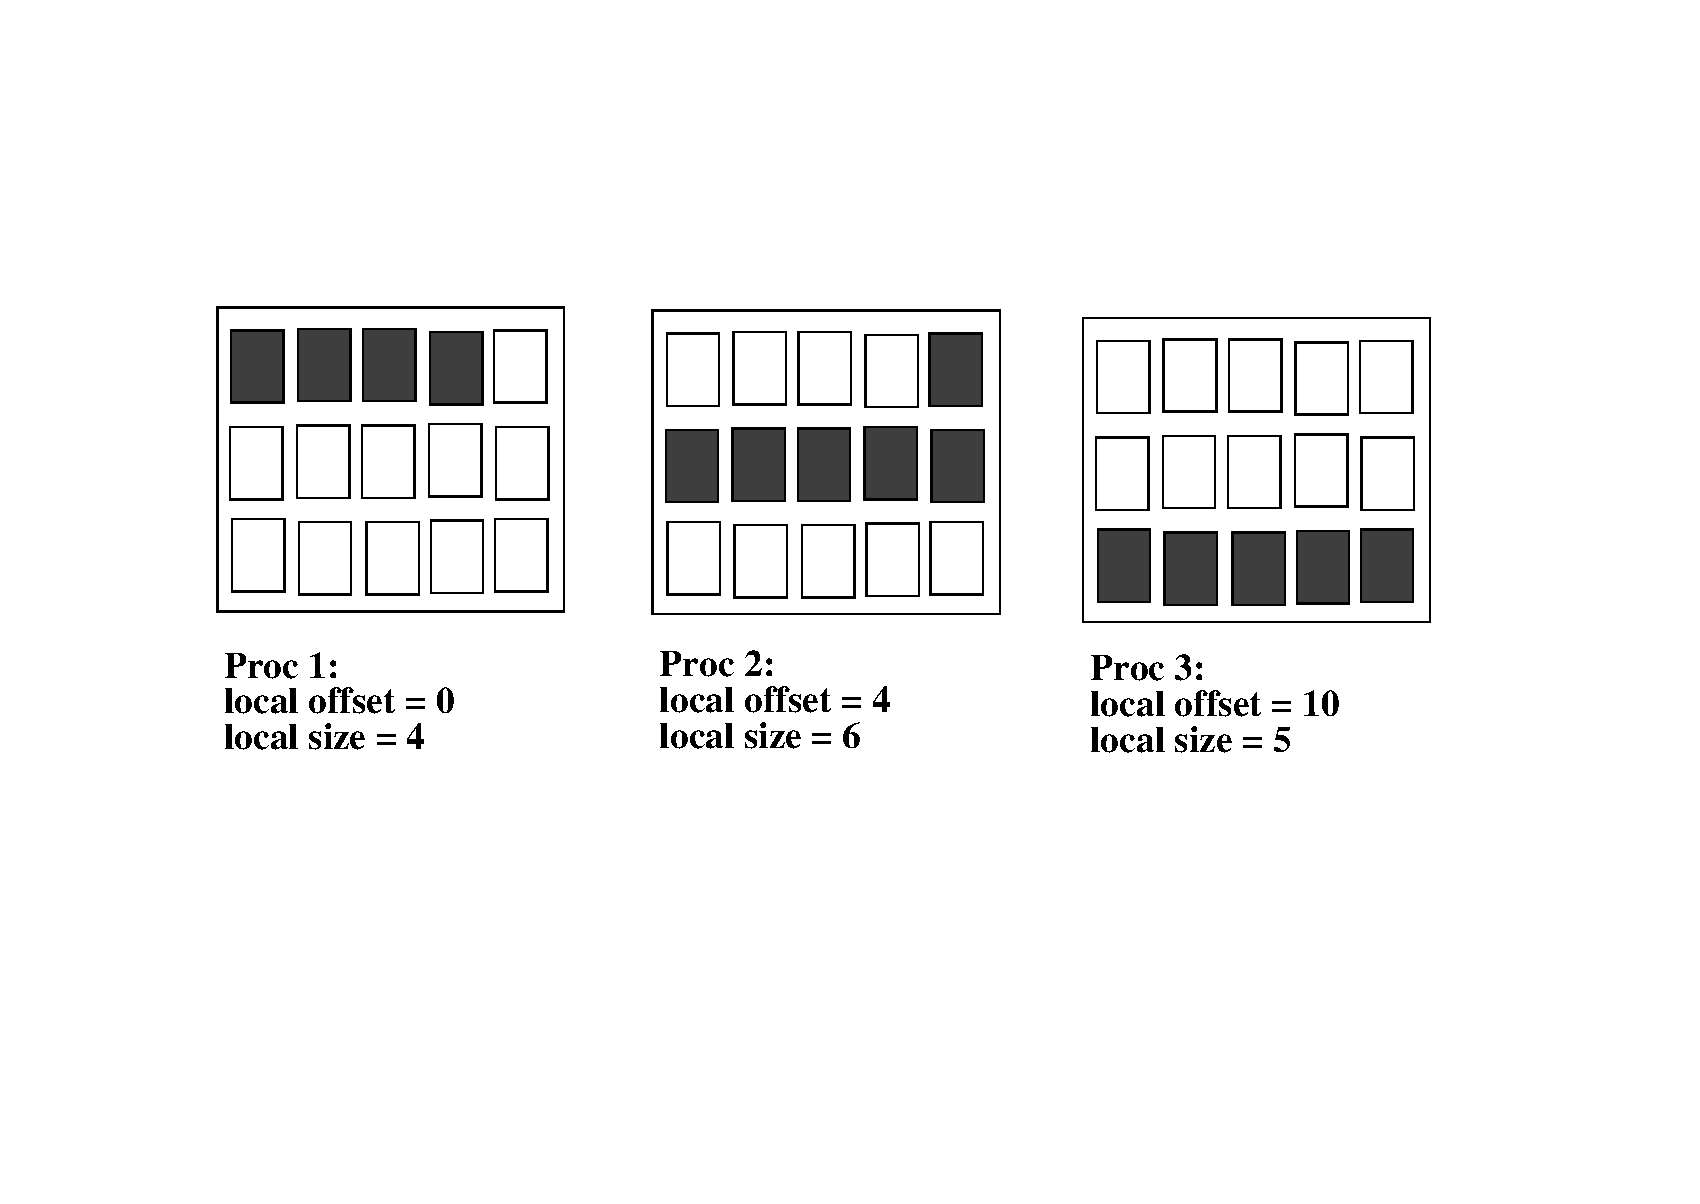
\includegraphics[scale=.6]{figures/apple_new}
  \caption{Apple partition. It is assumed here that the global index starts at
    0 in the upper left corner.}
  \label{apple_partition}
\end{figure}


\subsubsection{Box partition}

Each partition is a rectangular region of the global domain, described
by the global offset of its upper left corner, and its local extents
in the X and Y dimensions. The global extent in the X dimension must
also be given. In this case, we have {\tt ig\_paral(1:5)}:
\begin{itemize}
\item {\tt ig\_paral(1)} = 2 (indicates a Box partition)
\item {\tt ig\_paral(2)} = the upper left corner global offset
\item {\tt ig\_paral(3)} = the local extent in x
\item {\tt ig\_paral(4)} = the local extent in y
\item {\tt ig\_paral(5)} = the global extent in x.
\end{itemize}

Figure \ref{box_partition} illustrates a Box partition over 3
processes.
 
\begin{figure}
  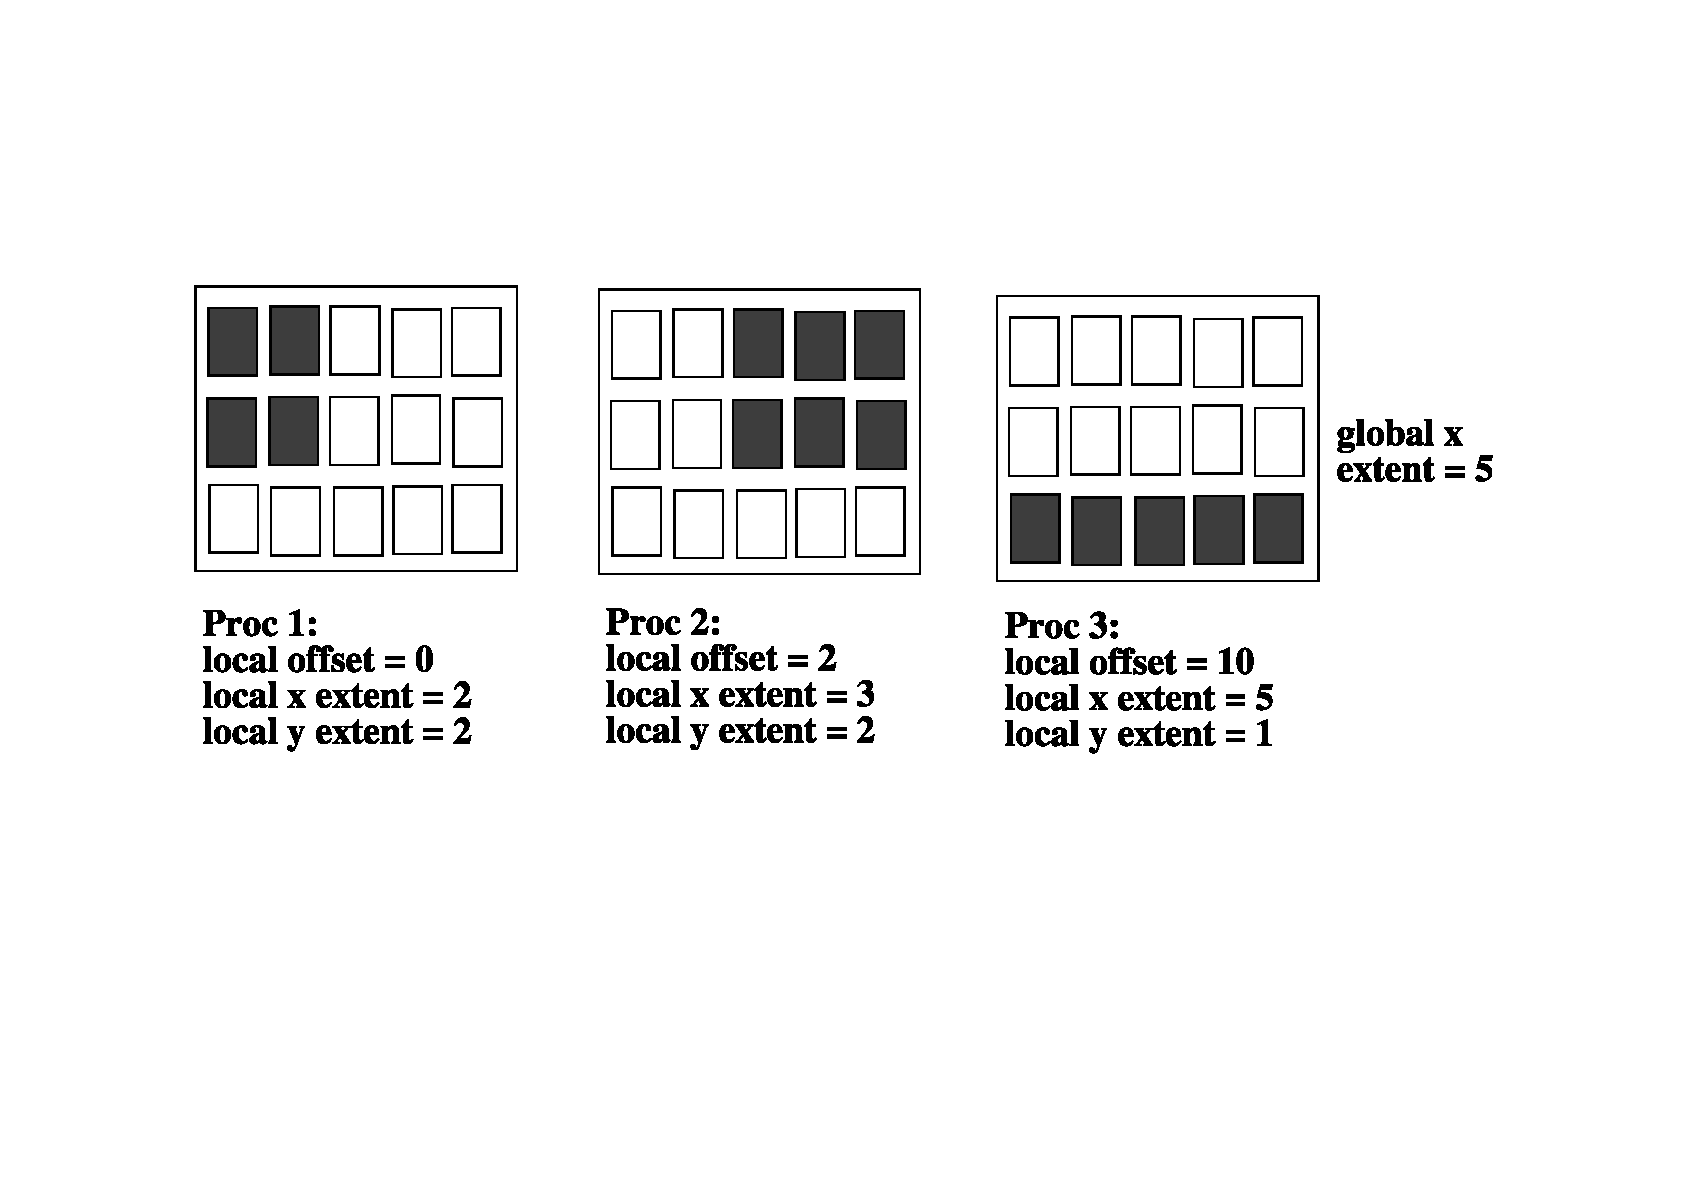
\includegraphics[scale=.6]{figures/box_new}
  \caption{Box partition. It is assumed here that the global index starts at 0
    in the upper left corner.}
  \label{box_partition}
\end{figure}
  
\subsubsection{Orange partition}

Each partition is an ensemble of segments in the global domain. Each
segment is described by its global offset and its local extent.  In
this case, we have {\tt ig\_paral(1:N)} where {\tt N = 2 + 2*number of
  segments}
% \footnote{As for the Box partition, the maximum number of segments
%   is presently 338; it can be increased by modifying the value of
%   {\tt Clim\_MaxSegments}}.

\begin{itemize}
\item {\tt ig\_paral(1)} = 3 (indicates a Orange partition)
\item {\tt ig\_paral(2)} = the total number of segments for the
  partition (limited to 200 presently, see note for ig\_paral(4) for
  Box partition above)
\item {\tt ig\_paral(3)} = the first segment global offset
\item {\tt ig\_paral(4)} = the first segment local extent
\item {\tt ig\_paral(5)} = the second segment global offset
\item {\tt ig\_paral(6)} = the second segment local extent
\item ...
\item {\tt ig\_paral(N-1)} = the last segment global offset
\item {\tt ig\_paral(N)} = the last segment local extent
\end{itemize}

Figure \ref{orange_partition} illustrates an Orange partition with 3
segments for one process. The other process partitions are not
illustrated.

\begin{figure}
  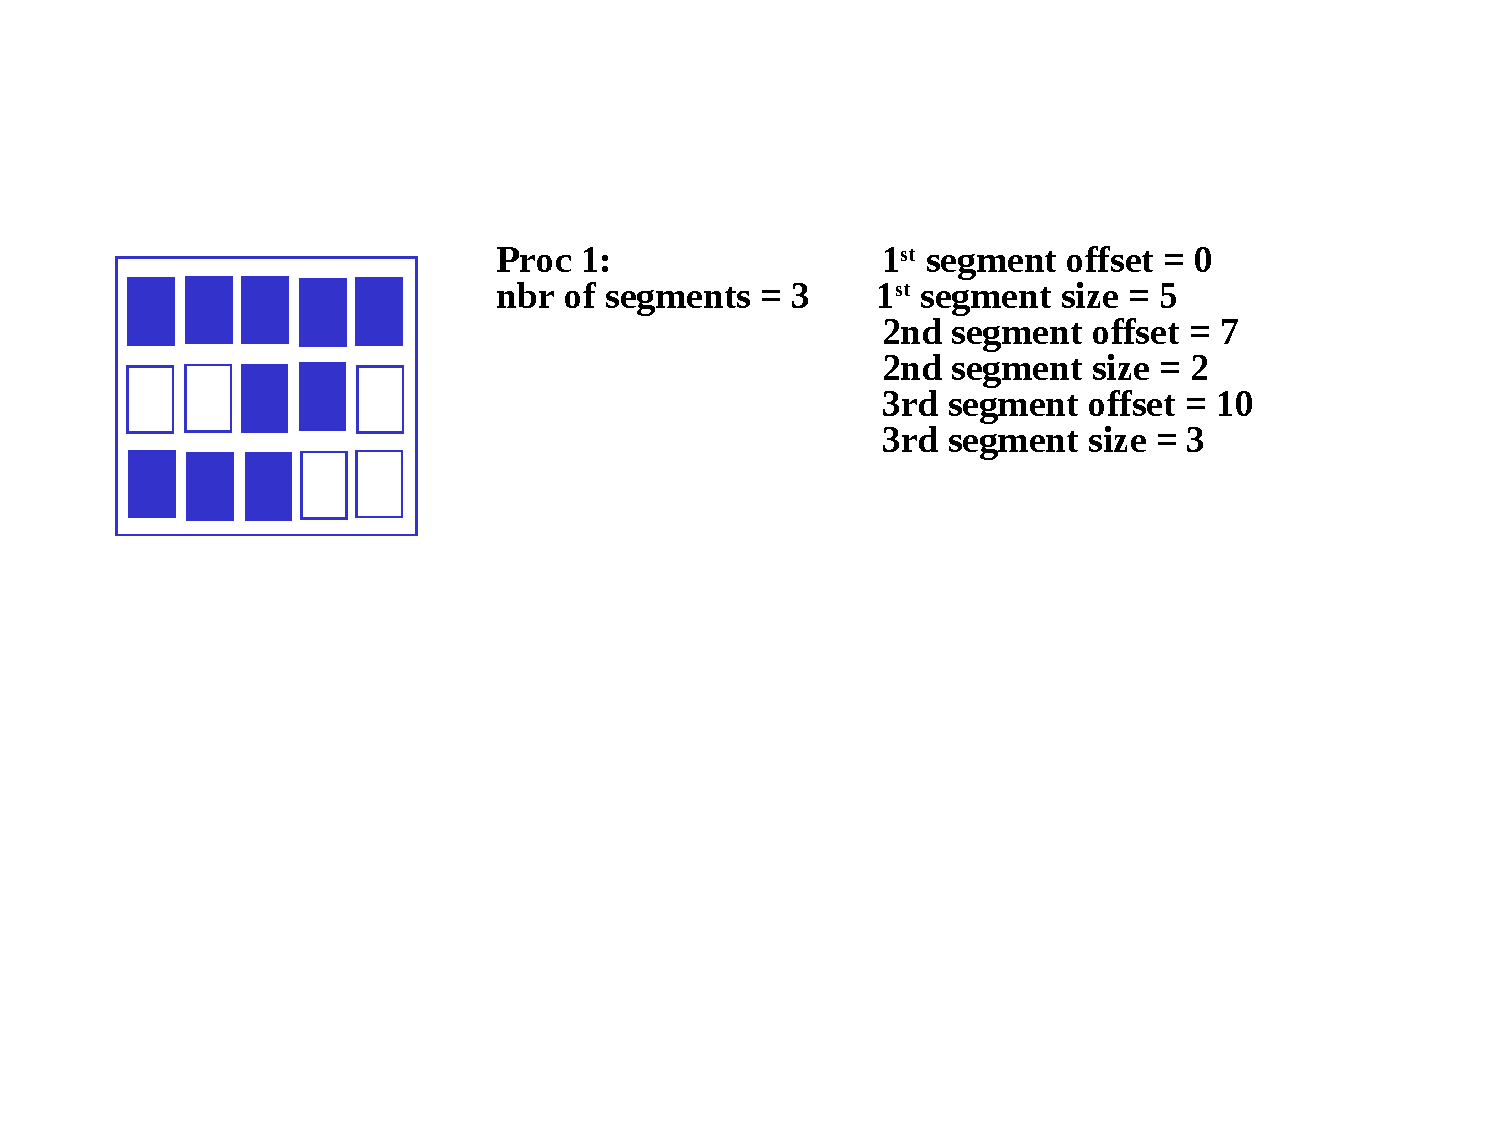
\includegraphics[scale=.6]{figures/orange_new}
  \caption{Orange partition for one process. It is assumed here that
    the global index starts at 0 in the upper left corner.}
  \label{orange_partition}
\end{figure}

\subsubsection{Points partition}

This partition is a list of global indices associated with each
process.  The index naming
is arbitrary but must be consistent between all processes involved
in the partition description.  In
this case, we have {\tt ig\_paral(1:N)} where {\tt N = 2 + number of
  points}
% \footnote{As for the Box partition, the maximum number of segments
%   is presently 338; it can be increased by modifying the value of
%   {\tt Clim\_MaxSegments}}.

\begin{itemize}
\item {\tt ig\_paral(1)} = 4 (indicates a Points partition)
\item {\tt ig\_paral(2)} = number of points in the partition 
\item {\tt ig\_paral(3)} = the first global index
\item {\tt ig\_paral(4)} = the second global index
\item ...
\item {\tt ig\_paral(N)} = the last global index
\end{itemize}

% {Partition definition}
\subsection{Grid data file definition}
\label{subsubsec_griddef}

Grid data files (see section \ref{subsec_griddata}) are required by OASIS3-MCT for specific operations , i.e.  {\em grids.nc} and {\em masks.nc} for
{\tt SCRIPR} (see section \ref{subsec_interp}), and {\em masks.nc} and
{\em areas.nc} for {\tt CONSERV} (see section
\ref{subsec_cooking}). These grid data files can be created by the
user before the run or can be written directly at run time by the components with the following routines.
If a grid data files does not exist, the corresponding routine will create it; if the grid data file exists, the routine can be used to {\bf add} grid definition fields but it will not {\bf overwrite} grid definition fields already existing in the file with the same grid name. 

These routines can be called only by one component process to write the whole grid or by each process holding a part of a grid. In the former case, optional argument {\tt il\_part\_id} is not needed and the arrays (see below) handling the longitudes of the grid points or corners ({\tt lon}, {\tt clon}), the latitudes of the grid points or corners ({\tt lat}, {\tt clat}), the masks ({\tt mask}) and areas ({\tt area}) of the grid cells need to cover the whole grid; in the later case, the {\tt il\_part\_id} returned by {\tt oasis\_def\_partition} needs to be provided as input argument and the arrays need to cover only the local partition of the grid .

\begin{itemize}

\item {\tt CALL oasis\_start\_grids\_writing (flag)} or
\item {\tt CALL prism\_start\_grids\_writing (flag)}
  \begin{itemize}
  \item {\tt flag [INTEGER; OUT]}: always 1 
  \end{itemize} 
Must be called to start the grid writing process. 
  
  \vspace{0.2cm}
\item {\tt CALL oasis\_write\_grid (cgrid, nx\_global, ny\_global, lon, lat, il\_part\_id)}
\item {\tt CALL prism\_write\_grid (cgrid, nx\_global, ny\_global, lon, lat, il\_part\_id)}
        
  \begin{itemize}
  \item {\tt cgrid [CHARACTER; IN]}: grid name prefix (see
    \ref{subsec_namcouplesecond} and \ref{subsec_griddata}); maximum length of 64 characters (4 are usually used for historical reasons)
  \item {\tt nx\_global [INTEGER; IN]} : first dimension of the global grid 
  \item {\tt ny\_global [INTEGER; IN]} : second dimension of the global grid ({\tt =0} if the grid is expressed as a 1D vector) 
  \item {\tt lon [REAL, DIMENSION(nx,ny); IN]} : single or double real array of longitudes covering the whole grid ({\tt nx=nx\_global}, {\tt ny=ny\_global}) or only the local partition (degrees East).
  \item {\tt lat [REAL, DIMENSION(nx,ny); IN]} : single or double real array of latitudes covering the whole grid ({\tt nx=nx\_global}, {\tt ny=ny\_global}) or only the local partition (degrees North)
\item  {\tt il\_part\_id [INTEGER, OPTIONAL; IN]}: partition ID returned by {\tt oasis\_def\_partition}, see \ref{subsubsec_Partition}; needed if each component task holding a part of a decomposed grid writes its own part of the grid.
  \end{itemize}

  Writes the component grid longitudes and latitudes. Longitudes must be
  given in degrees East in the interval -360.0 to 720.0. Latitudes
  must be given in degrees North in the interval -90.0 to 90.0. Note
  that if some grid points overlap, it is recommended to define those
  points with the same number (e.g. 90.0 for both, not 450.0 for one
  and 90.0 for the other) to ensure automatic detection of overlap by
  OASIS3-MCT (which is essential to have a correct conservative
  remapping \texttt{SCRIPR/CONSERV}, see section \ref{subsec_interp}).

  \vspace{0.2cm}
\item {\tt CALL oasis\_write\_corner (cgrid, nx\_global, ny\_global, nc, clon, clat, il\_part\_id))}
\item {\tt CALL prism\_write\_corner (cgrid, nx\_global, ny\_global, nc, clon, clat, il\_part\_id))}

  \begin{itemize}
  \item {\tt cgrid }, {\tt nx\_global }, {\tt ny\_global }, {\tt il\_part\_id }: as for {\tt oasis\_write\_grid}

  \item {\tt nc [INTEGER; IN]} : number of corners per grid cell
    (always 4 in the version)
  \item {\tt clon [REAL, DIMENSION (nx,ny,nc);IN]} : single or double real array of corner
    longitudes covering the whole grid ({\tt nx=nx\_global}, {\tt ny=ny\_global}) or only the local partition (in degrees\_East)
  \item {\tt clat [REAL, DIMENSION (nx,ny,nc);IN]} : single or double real array of corner
    latitudes covering the whole grid ({\tt nx=nx\_global}, {\tt ny=ny\_global}) or only the local partition (in degrees\_North)
  \end{itemize}

  Writes the grid cell corner longitudes and latitudes
  (counterclockwise sense). Longitudes must be given in degrees East
  in the interval -360.0 to 720.0. Latitudes must be given in degrees
  North in the interval -90.0 to 90.0. Note also that cells larger
  than 180.0 degrees in longitude are not supported. Writing of
  corners is optional as corner information is needed only for {\tt
    SCRIPR/CONSERV} (see section \ref{subsec_interp}). If called,
  needs to be called after {\tt oasis/prism\_write\_grid}.

  \vspace{0.2cm}
\item {\tt CALL oasis\_write\_mask (cgrid, nx\_global, ny\_global, mask, il\_part\_id)}
\item {\tt CALL prism\_write\_mask (cgrid, nx\_global, ny\_global, mask, il\_part\_id)}

  \begin{itemize}
  \item {\tt cgrid }, {\tt nx\_global }, {\tt ny\_global }, {\tt il\_part\_id }: as for {\tt oasis\_write\_grid}
  \item {\tt mask [INTEGER, DIMENSION(nx,ny) ;IN]} : mask array covering the whole grid ({\tt nx=nx\_global}, {\tt ny=ny\_global}) or only the local partition (be
    careful about the OASIS historical convention (!): 0 = not masked,
    1 = masked)
  \end{itemize}
  Writes the component grid mask.

  \vspace{0.2cm}
\item {\tt CALL oasis\_write\_area (cgrid, nx\_global, ny\_global, area, il\_part\_id)}
\item {\tt CALL prism\_write\_area (cgrid, nx\_global, ny\_global, area, il\_part\_id)}

  \begin{itemize}
  \item {\tt cgrid }, {\tt nx\_global }, {\tt ny\_global }, {\tt il\_part\_id }: as for {\tt oasis\_write\_grid}
  \item {\tt area [REAL, DIMENSION(nx,ny); IN]} : single or double real array of grid cell
    areas covering the whole grid ({\tt nx=nx\_global}, {\tt ny=ny\_global}) or only the local partition 
  \end{itemize}
  Writes of the component grid cell areas. Needed only for {\tt CONSERV}
  operation (see section \ref{subsec_cooking}).

  \vspace{0.2cm}
\item {\tt CALL prism\_terminate\_grids\_writing()} or
\item {\tt CALL oasis\_terminate\_grids\_writing()}

\end{itemize}

The creation of the different grid data files is effective in the routine
oasis\_enddef.

\subsection{Coupling field declaration}
\label{subsubsec_Declaration}

All processes of a component that send or receive a coupling field, or a part of it, needs to declare the coupling field.
 
Processes not implied in the
coupling do not have to call this routine at all (for backward
compatibility with OASIS3-MCT\_2.0, they may still call it with any {\tt name} and {\tt il\_part\_id}).

\begin{itemize}

\item {\tt CALL oasis\_def\_var (var\_id, name, il\_part\_id,
    var\_nodims, kinout, \newline var\_actual\_shape, var\_type,
    ierror)} or

\item {\tt CALL prism\_def\_var\_proto(var\_id, name, il\_part\_id,
    var\_nodims, kinout, var\_actual\_shape, var\_type, ierror)}

  \begin{itemize}
  \item {\tt var\_id [INTEGER; OUT]}: coupling field ID.  Note that all 
      coupling fields appearing in the {\it namcouple} must be defined with 
      a call to {\tt oasis\_def\_var}; not doing so would lead to an abort.  
      But all fields defined with a call to {\tt oasis\_def\_var} must not necessarily 
      appear in the {\it namcouple}. If a field does not appear in the {\it namcouple}, 
      the {\tt var\_id} returned by the {\tt oasis\_def\_var} will be equal to -1; 
      the value of the {\tt var\_id} should be tested and the corresponding 
      {\tt oasis\_put} and {\tt oasis\_get} should not be called if {\tt var\_id} 
      equals -1. These constraints are imposed to avoid that a typo in the {\it namcouple}
       would lead to coupling exchanges not corresponding to what the user intends to activate. 
  \item {\tt name [CHARACTER; IN]}: field symbolic name (as in the
    {\it namcouple}); maximum length of 80 characters
  \item {\tt il\_part\_id [INTEGER; IN]}: partition ID returned from {\tt oasis\_def\_partition} (see section
    \ref{subsubsec_Partition})
  \item {\tt var\_nodims [INTEGER, DIMENSION(2); IN]}: var\_nodims(1)
    is not used anymore in OASIS3-MCT so its value can be anything but
    it is still part of the oasis\_def\_var arguments; var\_nodims(2) is the number
    of fields in a bundle (this will be 1 for unbundled fields or greater
    than 1 for fields that are bundled).  
  \item {\tt kinout [INTEGER; IN]}: {\tt OASIS\_In} or {\tt PRISM\_In}
    (i.e. = 21) for fields received by the component; {\tt OASIS\_Out},
    {\tt PRISM\_Out} (i.e. = 20) for fields sent by the component
    \footnote{Parameters OASIS\_In, PRISM\_In, OASIS\_Out, PRISM\_Out
      are defined in
      oasis3-mct/lib/psmile/src/mod\_oasis\_parameters.F90}.
  \item {\tt var\_actual\_shape [INTEGER, DIMENSION(:), IN]}:
    not used anymore; vector of integers of any length (for simplicity
    we advise to pass any simple integer as argument)
  \item {\tt var\_type [INTEGER; IN]}: type of coupling field array;
    put {\tt OASIS\_Real} or {\tt PRISM\_Real} (i.e. = 4) for single
    or double precision real arrays.  All coupling data is treated as
    double precision in the coupling layer, but conversion to or from
    single precision data is supported in the interface.
  \item {\tt ierror [INTEGER; OUT]}: returned error code.
  \end{itemize}
\end{itemize}
% {coupling field declaration}

\subsection{End of definition phase}
\label{subsubsec_Endofdefinition}
All processes of components at least partly involved in the coupling (e.g. {\tt comp3} in figure
    \ref{Fig_coupling_layouts_b}) have to close the definition phase. Different configurations of components and corresponding use of {\tt oasis\_enddef} are described in section \ref{sec_deploy} and on figures \ref{Fig_coupling_layouts_a} and \ref{Fig_coupling_layouts_b}.
\begin{itemize}
\item {\tt CALL oasis\_enddef (ierror)}
\item {\tt CALL prism\_enddef\_proto(ierror)}
  \begin{itemize}
  \item ierror [INTEGER; OUT]: returned error code.
  \end{itemize}
\end{itemize}

% {End of definition phase}

\subsection{Sending ``put'' and receiving ``get'' actions}
\label{subsubsec_sendingreceiving}

This section describes how to send (put) and receive (get) fields through
the coupling interface.  This interface supports several ranks and
types of coupling fields.  First, the fields passed into the interface can be 
4 byte or 8 byte reals. The field decomposition must be 
consistent with the decomposition defined in the grid partition (see \ref{subsubsec_Partition})\footnote{But the decomposition of each field can be either one
dimensional or two dimensional and does not
have to match the rank of the grid partition.}  Third, the fields
can be bundled, i.e. have an extra (non-spatial) dimension like for a field covering different ice categories.  The bundled dimension is always the last dimension in any
field passed into the get and put routines.  And the size of the bundle dimension
must match the value defined for the variable in var\_nodims(2) in the
{\tt oasis\_def\_var} interface (see section \ref{subsubsec_Declaration}).

So in general, the fields passed into the get and put interface can have rank
1, 2, or 3 and include the following possible options where fld can be a 4
byte or 8 byte real array.

\begin{itemize}
\item 1D, fld(:) = an single, unbundled field of decomposition rank 1.
\item 2D, fld(:,:) = a single, unbundled field of decomposition rank 2.
\item 1D bundled, fld(:,:) = a bundled set of fields of decomposition rank 1.
  The size of the second dimension must equal the number of fields in the 
  bundle, defined by var\_nodims(2) in the {\tt oasis\_def\_var} interface.
\item 2D bundled, fld(:,:,:) = a bundled set of fields of decomposition rank 2.
  The size of the third dimension must equal the number of fields in the 
  bundle, defined by var\_nodims(2) in the {\tt oasis\_def\_var} interface.
\end{itemize}

%With bundled fields, it is important that the number of fields in the bundle match
%in the two models being coupled.  This requires that the var\_nodims(2) values
%in the send and receive model match the bundle dimension of that bundled coupling field.
Different bundled fields
can have different numbers of fields, but for a given bundled field, the
number of fields must match on the send and receive side.  This is explicitly
checked within the coupling layer and will lead to an abort if not done correctly.
It is possible to define a 1D bundled or 2D bundled field  with a bundle dimension of 1, i.e. for a bundle that contains only one single field.

Finally, the bundled field option can be used to
bundle together multi-level variables, multiple related fields, and other types
of fields.  The fields must share a common partition and common namcouple settings (e.g. interpolation)
to be bundled.  While this is a useful feature for multi-level fields, {\bf this does not mean
that 3D interpolation is supported}.
Each field in the bundle is
treated internally as a separate field in the coupling layer without
any information about the relationship between the fields in the bundle.  In fact,
the bundled field variables are internally renamed and a field number is appended
to the variable name to keep track of the distinct fields in the bundle.  That
updated variable name will appear in restart and output files.


\subsubsection{Sending a coupling (or I/O) field or writing a coupling restart file}
\label{prismput}

In the component time step loop, each process sends its part of the
coupling (or I/O) field.

\begin{itemize}
\item {\tt CALL oasis\_put (var\_id, date, fld1, info, fld2, fld3,
    fld4, fld5, write\_restart)}
\item {\tt CALL prism\_put\_proto(var\_id, date, fld1, info, fld2,
    fld3, fld4, fld5, write\_restart)}
  \begin{itemize}
  \item {\tt var\_id [INTEGER; IN]}: field ID (returned from corresponding {\tt
      oasis\_def\_var}, see section \ref{subsubsec_Declaration})
  \item {\tt date [INTEGER; IN]}: number of seconds (or any other time
    units as long as the same are used in all components and in the {\it
      namcouple}) at the time of the call (by convention at the
    beginning of the timestep)
  \item {\tt fld1 [REAL, IN]}: coupling (or I/O) field array; can be
    1D, 2D, bundled 1D, or bundled 2D, see baove. 
  \item {\tt info [INTEGER; OUT]}: returned info code:
    \begin{itemize}
    \item {\tt OASIS\_Sent} (=4) if the field was sent to another component
    \item {\tt OASIS\_LocTrans} (=5) if the field was only used in a time
      transformation (not sent, not output)
    \item {\tt OASIS\_ToRest} (=6) if the field was written to a restart
      file only
    \item {\tt OASIS\_Output} (=7) if the field was written to an output
      file only
    \item {\tt OASIS\_SentOut} (=8) if the field was both written to an
      output file and sent to another component 
    \item {\tt OASIS\_ToRestOut} (=9) if the field was written both to a
      restart file and to an output file.
    \item {\tt OASIS\_WaitGroup} (=14) if the field was not sent because it is part of a group.
    It will be sent only when the {\tt oasis\_put} of the last field in the group will be called; however, the field is buffered and therefore the field array can be modified in the component code when returning from the oasis\_put call.
    \item {\tt OASIS\_Ok} (=0) otherwise and no error occurred.
    \end{itemize}
  \item {\tt fld2 [REAL, IN, OPTIONAL]}: optional $2^{nd}$ coupling
    field array; can be 1D, 2D, bundled 1D, or bundled 2D.  Rank and size
    must match {\tt fld1}.
  \item {\tt fld3 [REAL, IN, OPTIONAL]}: optional $3^{rd}$ coupling
    field array; can be 1D, 2D, bundled 1D, or bundled 2D.  Rank and size
    must match {\tt fld1}.
  \item {\tt fld4 [REAL, IN, OPTIONAL]}: optional $4^{th}$ coupling
    field array; can be 1D, 2D, bundled 1D, or bundled 2D.  Rank and size
    must match {\tt fld1}.
  \item {\tt fld5 [REAL, IN, OPTIONAL]}: optional $5^{th}$ coupling
    field array; can be 1D, 2D, bundled 1D, or bundled 2D.  Rank and size
    must match {\tt fld1}.
  \item {\tt write\_restart [LOGICAL, IN, OPTIONAL]}: optional argument to write an 
    intermediate restart file associated with the variable {\tt
      var\_id} at the current timestep (see below).
  \end{itemize}
\end{itemize}

To ensure a proper use of the {\tt oasis\_put}, one has to take care
of the following aspects:

\begin{itemize}

\item A $2^{nd}$, $3^{rd}$, $4^{th}$ and $5^{th}$ source field can be
  passed as optional arguments. If so, the $2^{nd}$, $3^{rd}$,
  $4^{th}$ and $5^{th}$ set of weights present in the remapping file
  will be applied, respectively (see section \ref{subsec_mapdata} for
  the remapping file format). This will be used for example for the {\tt
    SCRIPR/BICUBIC} remapping for which a $1^{st}$, $2^{nd}$,
  $3^{rd}$, $4^{th}$ set of weights should be respectively applied to
  the field value, its gradient in the first dimension, its gradient
  in the second dimension, and its cross-gradient. Bicubic and higher order
  remapping are therefore supported given that the higher order fields
  are provided at each time step as {\tt oasis\_put} arguments. Note
  that if {\tt fld3}, or {\tt fld4}, or {\tt fld5} are passed, {\tt fld2}, or {\tt fld3} and 
  {\tt fld2}, or {\tt fld4} and {\tt fld3} and {\tt fld2} must also be passed respectively.
  
\item {\bf Note that from OASIS3-MCT\_4.0 onwards, 
the number of weights in the remapping file and the number of fields in the coupling restart file 
(when such a file is needed) must strictly match the number of source fields passed to the 
oasis\_put .}

%\item Trying to send with {\tt oasis\_put} a field declared with a
%  {\tt oasis\_def\_var} but not defined in the configuration file {\it
%    namcouple} will lead to an abort. In this case, the field ID
%  returned by the {\tt oasis\_def\_var} is equal to -1 and the
%  corresponding {\tt oasis\_put} should not be called.

\item This routine may be called by the component at each timestep. The
  convention for the {\tt date} argument is to indicate the time at
  the beginning of the timestep. The sending is actually performed
  if the time obtained by adding the field lag ({\tt LAG} in the
  {\em namcouple}, if any, with {\tt LAG=0} by default) to the {\tt date} corresponds to a time at which it
  should be activated, given the coupling or I/O period indicated by
  the user in the {\it namcouple} (see section \ref{sec_namcouple}).

\item By convention, the first coupling
  of a run occurs at {\tt date=0} and the final coupling occurs
  at {\tt date = runtime-cpl\_period}, where {\tt runtime} is the total time of
  the run and {\tt cpl\_period} is the coupling period of the field indicated by
  the user in the {\it namcouple} (see section \ref{sec_namcouple}).

\item For a coupling
  field with a positive lag, the coupling restart file (see section
  \ref{subsec_restartdata}) is automatically overwritten by the {\tt
    oasis\_put} when the {\tt date+LAG=runtime}.

  % \item A field will not be sent at all if its coupling (or I/O)
  %   period indicated in the {\it namcouple} is greater than the
  %   total run time.

\item The total run time should match an integer number of coupling
  periods.

\item If a local time transformation is indicated for the field by the
  user in the {\it namcouple} (INSTANT, AVERAGE, ACCUMUL, T\_MIN or
  T\_MAX, see section \ref{sec_transformations}), it is automatically
  performed and the resulting field is finally sent at the coupling or
  I/O frequency.  For non-instant transformations, partially
  transformed fields will be written to the restart file at the end of
  the run for use on the next component startup, when needed.

\item A coupling field sent by a source component can be
  associated with more than one target field and component, if specified
  as so with different entries in the {\it namcouple} configuration
  file. In that case, the source component needs to send the field only
  once and the corresponding data will arrive at multiple targets as
  specified in the {\it namcouple}. Different coupling frequencies and
  transformations are allowed for different coupling exchanges of the
  same field. If coupling restart files are required (either if a {\tt
    LAG} or if a {\tt LOCTRANS} transformation is specified), it is
  mandatory to specify different files for the different fields.

\item Trying to send with {\tt oasis\_put} a field declared with a {\tt
  oasis\_def\_var} but not defined in the configuration file {\it
  namcouple} will lead to an abort. When a field is not defined in the {\it namcouple}, the field ID
returned by the {\tt oasis\_def\_var} is equal to -1 and the
corresponding {\tt oasis\_put} should not be called. 

\item Support to couple multiple fields via a single communication.
This is supported through colon delimited field lists in the namcouple (see \ref{subsubsec_secondEXPORTED}). 
All fields will use the namcouple settings for that entry. In the component
model codes, these fields are still sent ({\bf “put”}) one at a time. Inside
OASIS3-MCT, the fields are stored and a single mapping and send instruction is executed
for all fields. This is useful in cases where multiple fields have the same coupling transformations
and to reduce communication costs by aggregating multiple fields into a single communication.

This option does not put any constraint
on the order of the related {\tt oasis\_put} and {\tt oasis\_get} in the codes.

As they appear in one single entry line, these fields must share the same coupling restart file 
but this restart file may contain other fields.

\item The optional argument, {\tt write\_restart}, in the {\tt oasis\_put} routine is {\bf false} by default. 
If a user sets that argument to true, a restart file will be written for that field {\bf only for that timestep}. The {\tt write\_restart} 
will just save the data that exists at the time of the call, taking into account lags and LOCTRANS operations. In 
cases where multiple fields are coupled as a single operation in the model (indicated via a list of colon delimited 
fields in the {\it namcouple}, see \ref{subsubsec_secondEXPORTED}), users are encouraged to specify 
the {\tt write\_restart} flag on ALL {\tt oasis\_put} calls at a given
time for this set of fields.
Intermediate restarts will be created with a timestamp prepended to
their filename, like TA000003600\_rst4.nc or TC000014400\_rst4.nc. 
A restart file that starts with TA will be a restart file associated
with LOCTRANS operations. A restart 
file that starts with TC will be a restart file associated with
coupling operations. The 9 digit timestamp in 
the filename is the date in seconds at the time of the oasis\_put
call. The restart filename (ie. rst4.nc) 
defined in the namcouple for variables will be used to generate a filename for intermediate restart files.
\end{itemize}

\subsubsection{Receiving a coupling (or I/O) field}

In the component time stepping loop, each process receives its part of the
coupling field.

\begin{itemize}
 
\item {\tt CALL oasis\_get (var\_id, date, fld, info)}
\item {\tt CALL prism\_get\_proto(var\_id, date, fld, info)}
  \begin{itemize}
  \item {\tt var\_id [INTEGER; IN]}: field ID (returned by the corresponding
    {\tt oasis\_def\_var})
  \item {\tt date [INTEGER; IN]}: number of seconds (or any other time
    units as long as the same are used in all components and in the {\it
      namcouple}) at the time of the call (by convention at the
    beginning of the timestep)
  \item {\tt fld [REAL, OUT]}: I/O or coupling field array;  
    can be 1D, 2D, bundled 1D, or bundled 2D.
  \item {\tt info [INTEGER; OUT]}: returned info code:
    \begin{itemize}
    \item OASIS\_Recvd(=3) if the field was received from another
      component
    \item OASIS\_FromRest (=10) if the field was read from a restart
      file only
    \item OASIS\_Input (=11) if the field was read from an input file
      only
    \item OASIS\_RecvOut (=12) if the field was both received from
      another component and written to an output file
    \item OASIS\_FromRestOut (=13) if the field was both read from a
      restart file and written to an output file
    \item OASIS\_Ok (=0) otherwise and no error occurred.
    \end{itemize}
  \end{itemize}
\end{itemize}

To ensure a proper use of the {\tt oasis\_get}, one has to take care of the following aspects:

\begin{itemize}

\item This routine may be called by the component at each timestep. The {\tt
  date} argument is automatically analysed and the receiving action is
actually performed only if {\tt date} corresponds to a time for which
it should be activated, given the period indicated by the user in the
{\it namcouple}. An exchange at the beginning of the run at time=0 is
expected.

\item Trying to receive with {\tt oasis\_get} a field declared with a {\tt
  oasis\_def\_var} but not defined in the configuration file {\it
  namcouple} will lead to an abort. In this case, the field ID
returned by the {\tt oasis\_def\_var} is equal to -1 and the
corresponding {\tt oasis\_get} should not be called. 

\item If a coupling field has a positive lag, the coupling field that
  matches the {\tt oasis\_get} at time=0 will come from a coupling
  restart file written by the last active {\tt oasis\_put} of the
  previous run (see section \ref{subsubsec_Algoritms}). 

\item Support to couple multiple fields via a single communication.
This is supported through colon delimited field lists in the namcouple (see \ref{subsubsec_secondEXPORTED}). 
All fields will use the namcouple settings for that entry. In the component
model codes, these fields are still received (via an {\tt oasis\_get}) one at a time. Inside
OASIS3-MCT, the fields are stored and a single mapping and receive instruction is executed
for all fields. This is useful in cases where multiple fields have the same coupling transformations
and to reduce communication costs by aggregating multiple fields into a single communication. If a
LOCTRANS transformation is needed for these multiple fields, it is necessary to define a restart file
for these multiple fields.
\end{itemize}

\subsection{Termination}
\label{subsubsec_Termination}

\begin{itemize}

\item {\tt CALL oasis\_terminate (ierror)}
\item {\tt CALL prism\_terminate\_proto(ierror)}
  \begin{itemize}
  \item {\tt ierror [INTEGER; OUT]}: returned error code.
  \end{itemize}
All processes of components at least partly involved in the coupling (e.g. {\tt comp3} in figure
    \ref{Fig_coupling_layouts_b}) have to terminate the coupling by
  calling this routine\footnote{If the process called {\tt MPI\_Init}
    (before calling {\tt oasis\_init\_comp}), it must also call {\tt
      MPI\_Finalize} explicitly, but only after calling {\tt
      oasis\_terminate\_proto}.}(normal termination). Different configurations of components and corresponding use of {\tt oasis\_terminate} are described in section \ref{sec_deploy} and on figures \ref{Fig_coupling_layouts_a} and \ref{Fig_coupling_layouts_b}.

  

\end{itemize}

% {Termination}

\subsection{Auxiliary routines}
\label{subsubsec_auxroutines}

The following auxiliary routines are currently available.

\begin{itemize}
\item {\tt CALL oasis\_abort (compid, routine\_name, abort\_message, rcode)}
\item {\tt CALL prism\_abort\_proto(compid, routine\_name,
    abort\_message)}
  \begin{itemize}
  \item {\tt compid [INTEGER; IN]}: component ID (from {\tt
      oasis\_init\_comp})
  \item {\tt routine\_name[CHARACTER*; IN]}: name of calling routine
  \item {\tt abort\_message[CHARACTER*; IN]}: message to be written
    out.
  \item {\tt rcode [INTEGER, OPTIONAL; IN]}: Optional argument. When OASIS 
    aborts, it returns rcode if it is present, else it returns 1
  \end{itemize}

  If a process needs to abort voluntarily, it should do so by calling
  {\tt oasis\_abort}. This will ensure a proper termination of all
  processes in the coupled model communicator. This routine writes the
  name of the calling component, the name of the calling routine, and the
  message to the process debug file (see {\tt \$NLOGPRT} in section
  \ref{subsec_namcouplefirst}).  This routine cannot be called before
  {\tt oasis\_init\_comp}.

  \vspace{0.2cm}
\item {\tt CALL oasis\_get\_debug(debug\_value)}
\item {\tt CALL prism\_get\_debug(debug\_value)}
  \begin{itemize}
  \item {\tt debug\_value [INTEGER; OUT]}: debug value
  \end{itemize}

  This routine may be called at any time to retrieve the current
  OASIS3-MCT internal debug level (see {\tt \$NLOGPRT} in section
  \ref{subsec_namcouplefirst}).  This is useful if the user wants to
  return the original debug value after changing it.

  \vspace{0.2cm}
\item {\tt CALL oasis\_set\_debug(debug\_value)}
\item {\tt CALL prism\_set\_debug(debug\_value)}
  \begin{itemize}
  \item {\tt debug\_value [INTEGER; IN]}: debug value
  \end{itemize}

  This routine may be called at any time to change the debug level in
  OASIS3-MCT.  This method allows users to vary the debug level at
  different points in the component integration.

  \vspace{0.2cm}
\item {\tt CALL oasis\_get\_intercomm(new\_comm, cdnam, kinfo)}
\item {\tt CALL prism\_get\_intercomm(new\_comm, cdnam, kinfo)}
  \begin{itemize}
  \item {\tt new\_comm [INTEGER; OUT]}: mpi intercomm communicator
  \item {\tt cdnam [CHARACTER*; IN]}: other component name (i.e. 2nd argument of  the call to {\tt oasis\_init\_comp} in that component)
  \item {\tt kinfo [INTEGER; OUT; OPTIONAL]}: returned error code
  \end{itemize}

  This routine sets up an MPI intercomm communicator between the root
  processors of two components, the local component and the component
  associated with {\tt cdnam}.  This call is collective across the
  tasks of the two components but other components are not involved.

  \vspace{0.2cm}
\item {\tt CALL oasis\_get\_intracomm(new\_comm, cdnam, kinfo)}
\item {\tt CALL prism\_get\_intracomm(new\_comm, cdnam, kinfo)}
  \begin{itemize}
  \item {\tt new\_comm [INTEGER; OUT]}: mpi intracomm communicator
  \item {\tt cdnam [CHARACTER*; IN]}: other component name (i.e. 2nd argument of  the call to {\tt oasis\_init\_comp} in that component)
  \item {\tt kinfo [INTEGER; OUT; OPTIONAL]}: returned error code
  \end{itemize}

  This routine sets up an MPI intracomm communicator between the root
  processors of two components, the local component and the component
  associated with {\tt cdnam} .  This call is collective across the tasks of
  the two components but other components are not involved.

\item {\tt CALL oasis\_put\_inquire(var\_id, date, kinfo)}
\item {\tt CALL prism\_put\_inquire\_proto(var\_id, date, kinfo)}
  \begin{itemize}
  \item {\tt var\_id [INTEGER; IN]}: field ID (from
  corresponding oasis\_def\_var)
  \item {\tt date [INTEGER; IN]}: as in {\tt oasis\_put}, number of seconds (or any other time
    units as long as the same are used in all components and in the {\it
      namcouple}) in the run at the time of the call
  \item {\tt kinfo [INTEGER; OUT]}: returned info code
    \begin{itemize}
    \item OASIS\_Sent(=4) if the field would be sent to another component
    \item OASIS\_LocTrans (=5) if the field would be only used in a time
      transformation (not sent, not output)
    \item OASIS\_ToRest (=6) if the field would be written to a restart
      file only
    \item OASIS\_Output (=7) if the field would be written to an output
      file only
    \item OASIS\_SentOut (=8) if the field would be both written to an
      output file and sent to another component (directly or via OASIS3
      main process)
    \item OASIS\_ToRestOut (=9) if the field would be written both to a
      restart file and to an output file.
    \item OASIS\_Ok (=0) otherwise and no error occurred.
    \end{itemize}
  \end{itemize}

This routine may be called at any time to
inquire what would happen to the corresponding field (i.e. with same
{\tt var\_id} and at same {\tt date}) below the corresponding {\tt
  oasis\_put}. This maybe useful if, for example, the calculation of
a coupling field is costly and if one wants to compute it only when it is
really sent out.

\item {\tt CALL oasis\_get\_ncpl(var\_id, ncpl, kinfo)}
\item {\tt CALL prism\_get\_ncpl\_proto(var\_id, ncpl, kinfo)}
  \begin{itemize}
  \item {\tt var\_id [INTEGER; IN]}: field ID (from
  corresponding oasis\_def\_var)
  \item {\tt ncpl [INTEGER; OUT]}: number of coupling exchanges in which the field
  is involved (i.e. when a field is sent to multiple targets) 
  \item {\tt kinfo [INTEGER; OUT]}: returned info code
  \end{itemize}

This routine returns the number of coupling exchanges in which the field var\_id is
involved. This number is needed to get the coupling frequencies with the
routine oasis\_get\_freqs, see below.

\item {\tt CALL oasis\_get\_freqs(var\_id, ncpl, cpl\_freqs, kinfo)}
\item {\tt CALL prism\_get\_freqs\_proto(var\_id, ncpl, cpl\_freqs, kinfo)}
  \begin{itemize}
  \item {\tt var\_id [INTEGER; IN]}: field ID (from
  corresponding oasis\_def\_var)
  \item {\tt ncpl [INTEGER; IN]}: number of couplings in which the field
  is involved (i.e. when a field is sent to multiple targets)
   \item {\tt cpl\_freqs [INTEGER; DIMENSION(ncpl); OUT]}: coupling period(s) 
  (in number of seconds) of field var\_id. There is one coupling period for
  each coupling exchange in which the field is involved
  \item {\tt kinfo [INTEGER; OUT]}: returned info code
  \end{itemize}

This routine can be used to retrieve the coupling period(s) of field with
corresponding {\tt var\_id}, as defined in the {\it namcouple}

\end{itemize}

\section{Coupling algorithms - LAG and SEQ concepts}
\label{subsubsec_Algoritms}

Using the OASIS3-MCT coupling library, the user has full flexibility
to reproduce different coupling algorithms. In the components, the
sending and receiving routines, respectively {\tt oasis\_put} and {\tt
  oasis\_get}, can be called at each component timestep, with the
appropriate {\tt date} argument giving the actual time (at the
beginning of the timestep), expressed in number of seconds since the
start of the run, or in any other time units as long as the same are
used in all components and in the {\it namcouple} (see section
\ref{prismput}). This {\tt date} argument is automatically analysed by
the coupling library and depending on the coupling period and the lag chosen by the user for the coupling field in the {\it namcouple} ({\tt LAG}), different coupling algorithms can be reproduced
without modifying the component codes themselves.

With OASIS3-MCT, a sequence index specified for a coupling field in the {\it namcouple} ({\tt SEQ}), 
provides the coupling layer with an ability to detect a deadlock
before it happens and exit.

The LAG and SEQ concept are explained in more detail below and
some examples are provided.

\vspace{-0.3cm}
\subsection{The lag concept}
\label{subsub_lag}

The lag ({\tt LAG}) must be
expressed in the time unit used (that must be the same in the components
and in the {\it namcouple}, see section \ref{prismput}) and can be
positive or negative but should never be larger (in absolute
magnitude) than the coupling period of any field due to problems with
restartability and dead-locking. When a component calls a {\tt
  oasis\_put}, the value of the lag is automatically added to the
value of the {\tt date} argument and the ``put'' is actually performed
when the sum {\tt date+lag} is a coupling time; in the target
component, this ``put'' will match a {\tt oasis\_get} for which the
{\tt date} argument is the same coupling time.
% A positive lag indicates the put will occur sooner than zero lag and
% a negative lag tells the coupler to send the data later than zero
% lag.
So the lag only shifts the time at which the data is sent but not
the time at which the data is received.
 
When the lag is positive, a restart file must be available to initiate
the coupling.  For a field with positive lag, the source
component automatically reads the field in the restart file
during the coupling initialization phase (below the {\tt
  oasis\_enddef}) and send the data to match the {\tt oasis\_get}
performed at time=0 in the target component. The final coupling
data on the source side will then be automatically written to the
restart file for use in the next run\footnote{When there is a lag, the first and last instance of the source field
in the debug netCDF file (EXPOUT fields, see section
\ref{subsec_namcouplesecond}) always correspond respectively to the
field read from and written to the restart file.}.

On the 4 figures in this section, short black arrows correspond to
  {\tt oasis\_put} or {\tt oasis\_get} called in the component
  that do not lead to any ``put" or receiving action; long black
  arrows correspond to {\tt oasis\_put} or {\tt oasis\_get} called in
  the components that do actually lead to a ``put" or ``get''
  action; long red arrows correspond to {\tt oasis\_put} or {\tt
    oasis\_get} called in the component models that lead to a reading
  or writing of the coupling field from or to a coupling restart file.
 
\begin{enumerate}

\item LAG concept first example
 
  A first coupling algorithm, exploiting the LAG concept, is
  illustrated on figure \ref{fig:lag_concept_1}.

  

  \begin{figure}
    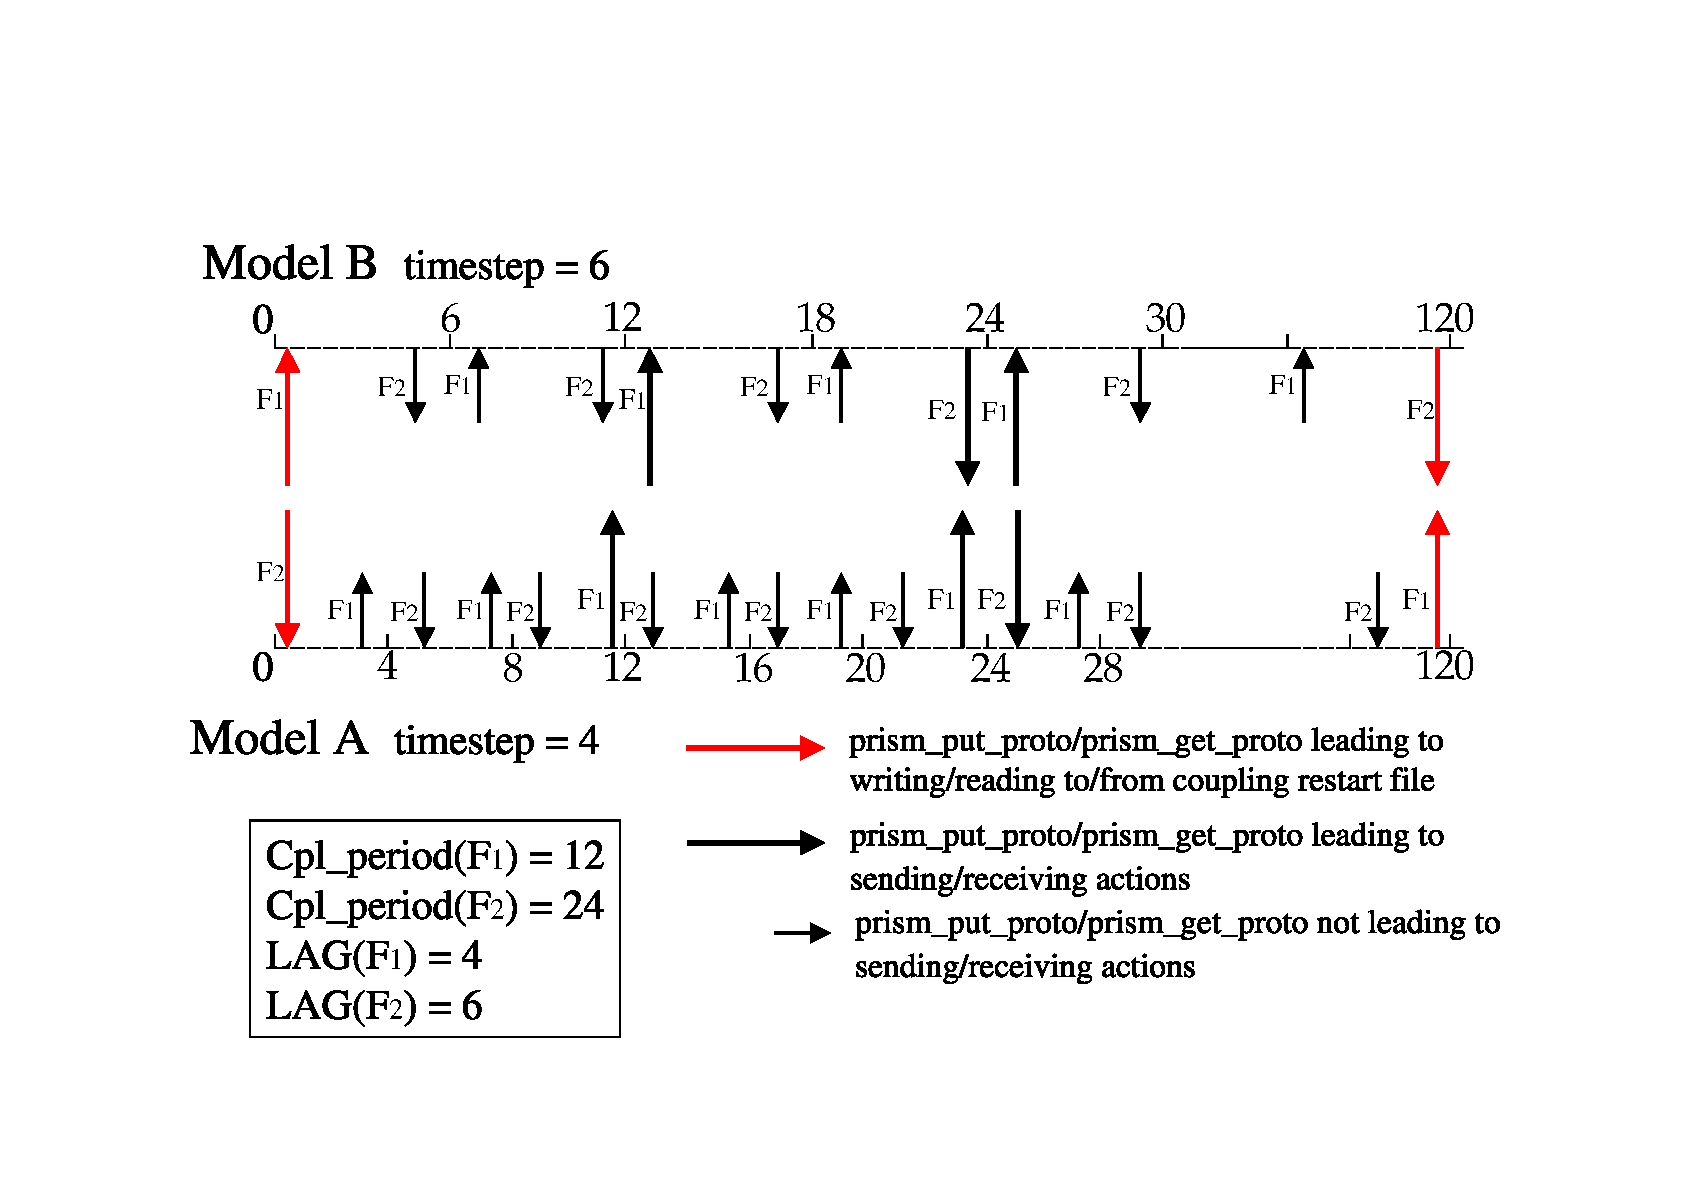
\includegraphics[scale=.6]{figures/fig_lag_concept_1}
    \caption{LAG concept first example}
    \label{fig:lag_concept_1}
  \end{figure}

  During a coupling timestep, model A receives $F_2$ and then sends
  $F_1$; its timestep length is 4. During a coupling timestep, model B
  receives $F_1$ and then sends $F_2$; its timestep length is 6.
  $F_1$ and $F_2$ coupling periods are respectively 12 and 24. If
  $F_1$/$F_2$ ``put" action by model A/B was used at a coupling
  timestep to match the model B/A ``get" action, a deadlock would
  occur as both models would be initially waiting on a ``get"
  action. To prevent this, $F_1$ and $F_2$ produced at the timestep
  before have to be used to match respectively the model B and model A
  ``get" actions.

  This implies that a lag of respectively 4 and 6 seconds must be
  defined for $F_1$ and $F_2$. For $F_1$, the {\tt oasis\_put}
  performed at time 8 and 20 by model A will then lead to ``put"
  actions (as 8 + 4 = 12 and 20 + 4 = 24 which are coupling periods)
  that match the ``get" actions performed by {\tt oasis\_get} called by model B
  at times 12 and 24.  For $F_2$, the {\tt oasis\_put}
  performed at time 18 by model B then leads to a ``put" action (as 18
  + 6 = 24 which is a coupling period) that matches the ``get" action
  performed at time 24 by the {\tt oasis\_get} called by model A.

  At the beginning of the run, as their LAG index is greater than 0,
  the first {\tt oasis\_get} of $F_1$ and $F_2$ will automatically be
  fulfilled with fields read from their respective coupling restart
  files. The user therefore has to create those coupling restart files
  before the first run in the experiment. At the end of the run, $F_1$
  having a lag greater than 0, is automatically written to its
  coupling restart file below the last $F_1$ {\tt oasis\_put} as the
  {\tt date+lag} equals the total run time. The analogue is true for
  $F_2$. These coupling restart fields will automatically be read in at the beginning
  of the next run below the respective {\tt oasis\_get}.

\item LAG concept second example

  A second coupling algorithm exploiting the LAG concept is
  illustrated on figure \ref{fig:lag_concept_2}. During its timestep,
  model A receives $F_2$, sends $F_3$ and then $F_1$; its timestep
  length is 6. During its timestep, model B receives $F_1$, receives
  $F_3$ and then sends $F_2$; its timestep length is also 6.  $F_1$,
  $F_2$ and $F_3$ coupling periods are both supposed to be equal to
  12.
 
  \begin{figure}
    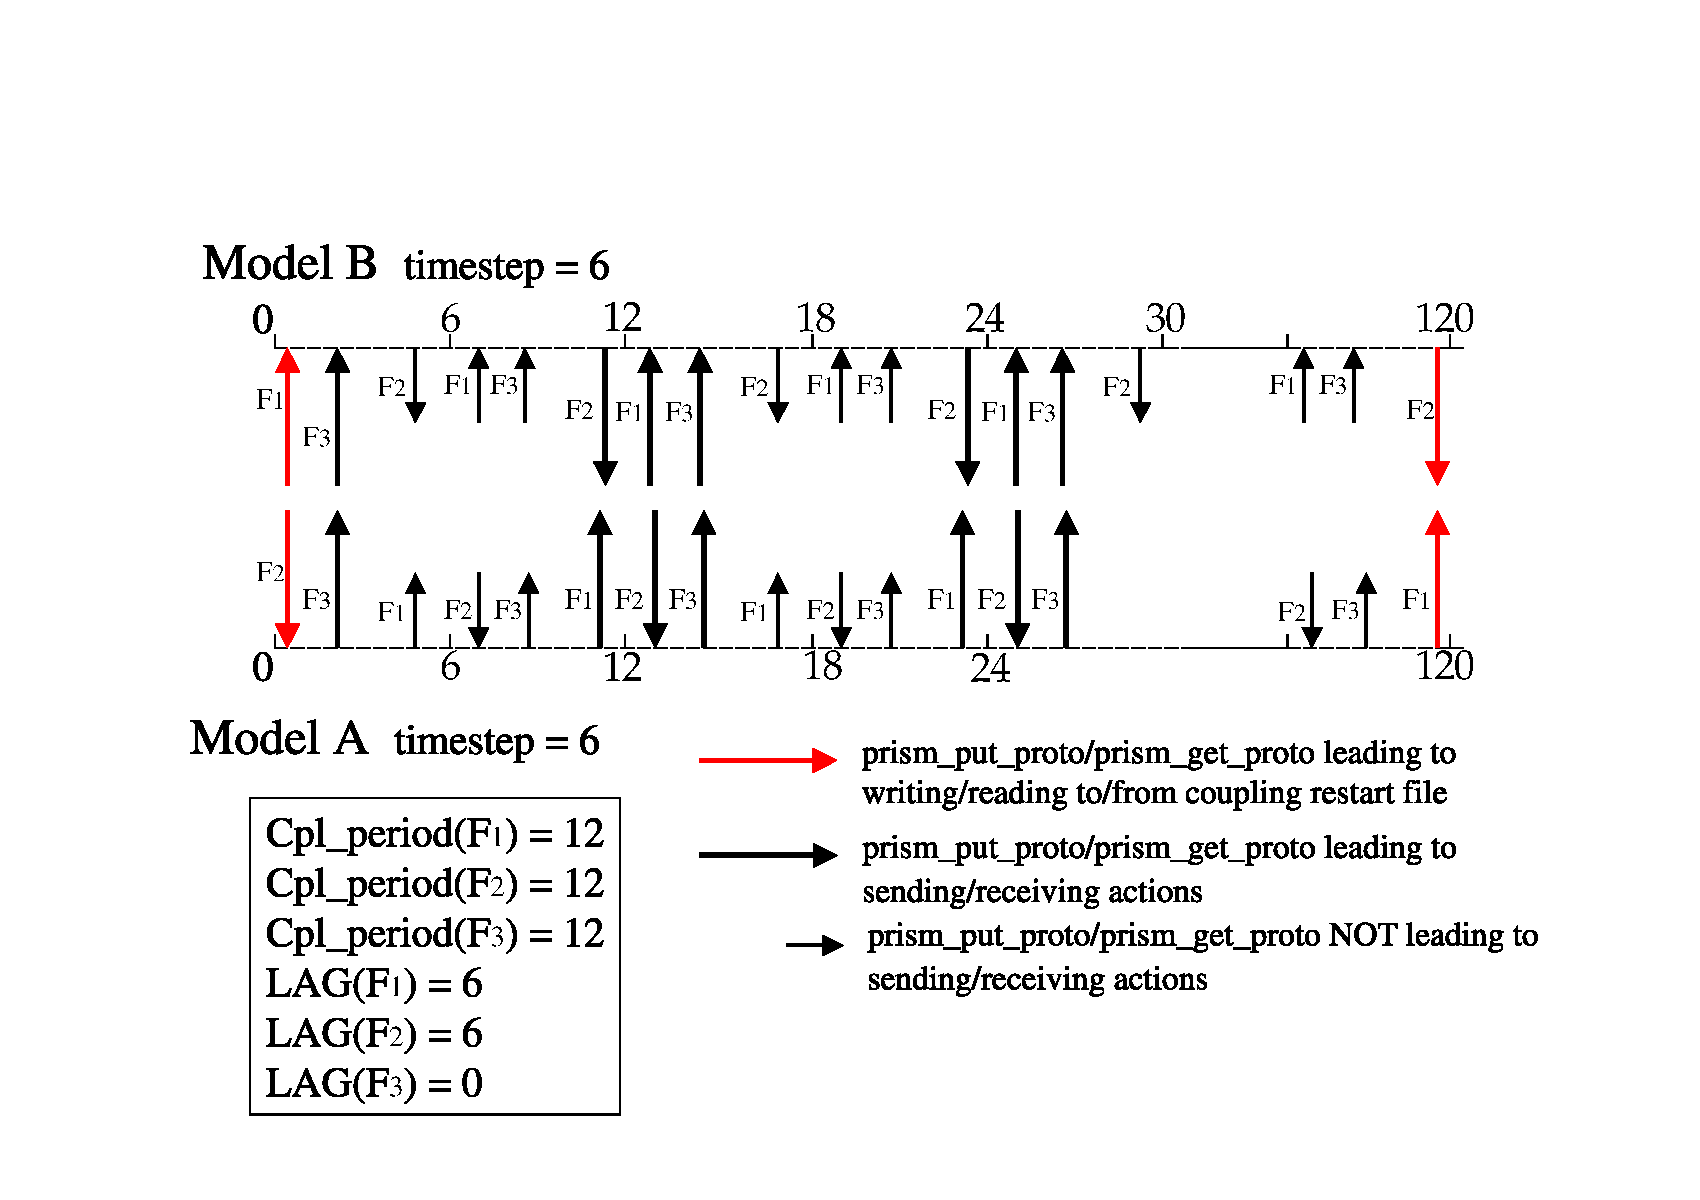
\includegraphics[scale=.6]{figures/fig_lag_concept_2}
    \caption{LAG concept second example}
    \label{fig:lag_concept_2}
  \end{figure}

  For $F_1$ and $F_2$ the situation is similar to the first
  example. Without any lag specified and without any restart file, a deadlock
  would occur as both models would be waiting on a ``get" action. To
  prevent this, $F_1$ and $F_2$ produced at the timestep before have
  to be used to match the model A and model B ``get" actions, which
  means that a lag of 6 must be defined for both $F_1$ and $F_2$. For
  both coupling fields, the {\tt oasis\_put} performed at times 6 and
  18 by the source model then lead to ``put" actions (as 6 + 6 = 12
  and 18 + 6 = 24 which are coupling periods) that match the ``get"
  action performed at time 12 and 24 by the {\tt oasis\_get} called
  by the target model.

  For $F_3$, sent by model A and received by model B, no lag needs to
  be defined: the coupling field produced by model A at the coupling
  timestep can be ``consumed'' by model B without causing a deadlock
  situation.

  As in the first example, the {\tt oasis\_get} performed at the
  beginning of the run for $F_1$ and $F_2$, will automatically receive
  data read from their coupling restart files, and the last {\tt
    oasis\_put} performed at the end of the run automatically write
  them to their coupling restart file. For $F_3$, no coupling restart
  file is needed.

  We see here how the introduction of appropriate LAG indices results
  in receiving in the target component the coupling fields produced by the
  source component the time step before; this is, in some coupling
  configurations, essential to avoid deadlock situations.

\end{enumerate}

\vspace{-0.3cm}
\subsection{The sequence concept}
\label{subsec_sec}

The order of coupling operations in the system is determined solely by
the order of calls to send ({\tt oasis\_put} or ``put'') and receive ({\tt oasis\_get} or ``get'') data in the components
in conjunction with the setting of the lag in the {\it namcouple}.
Data that is received is always blocking while data that is sent is non-blocking with respect to the component making that call.  It
is possible to deadlock the system if the relative orders of puts and
gets in different components are not compatible.

With OASIS3-MCT, the sequence (SEQ) index in the {\it namcouple} file
now provides the coupling layer with an ability to detect a deadlock
before it happens and exit.  It does this by tracking the order of get
and put calls in components compared to the SEQ specified in the {\it
  namcouple}.  If there are any inconsistencies, the component will abort
gracefully with a useable error message before the system deadlocks.
If there are any coupling dependencies in the system, use of the SEQ
index is recommended for diagnosis but has no impact on the ultimate
solution and is NOT required.

In the following two examples, there are two
models, each ``put" a field to the other at every coupling period
without any lags.  In the first case, there is no dependency as each
model first sends and then receives some data.

\begin{verbatim}
     model1        model2
     ------        ------
    put(fld1)     put(fld2)
    get(fld2)     get(fld1)
\end{verbatim}

In this
case, there is no sequencing dependency and the value of SEQ must be
identical (or unset) in the {\it namcouple} description of the fld1
and fld2 coupling.  If by mistake, SEQ is set to 1 for fld1 and 2 for fld2, 
then the coupled model will abort because at runtime, the coupler will
detect in model 2 that fld2 was sent before fld1 was received which
is out of sequence as defined by the SEQ settings.

In the next example, there is a dependency in the sequencing.

\begin{verbatim}
     model1        model2
     ------        ------
    put(fld1)     get(fld1)
                  fld2=g(fld1)
    get(fld2)     put(fld2)
\end{verbatim}

In model2, fld2 depends on fld1. If SEQ is not used and if, for example, model1 does not have the
consistent ordering of the put and get shown above (required by model2), then the models would deadlock and hang. If this dependency is known, there is a benefit in setting SEQ=1 for fld1 and SEQ=2 for fld2; at
runtime, if the sequencing of model1 or model2 does not match the
above diagram, then the  coupling layer will detect it and will exit gracefully with an error message.

Again, the SEQ namecouple setting is only diagnostic and is not
required.




\newpage
\chapter{The configuration file {\it namcouple}}
\label{sec_namcouple}

The OASIS3-MCT configuration file {\it namcouple} contains, below
pre-defined keywords, all user-defined information necessary to
configure a particular coupled run.

The {\it namcouple} is a text file with the following characteristics:

\begin{itemize}
\item the keywords used to separate the information can appear in any
  order;
\item the number of blanks between two character strings is
  non-significant;
\item all lines beginning with \# are ignored and considered as
  comments;
\item blank lines are supported, but only since OASIS3-MCT\_4.0 version.
\end{itemize}

The first part of {\it namcouple } is devoted to configuration of
general parameters such as the total run time or the desired debug level.  
The second part gathers specific
information on each coupling (or I/O) field, e.g. their coupling
period, the list of transformations or remapping to be performed
by OASIS3-MCT and associated configuring lines (described in more
details in chapter \ref{sec_transformations}).

In OASIS3-MCT, several {\it namcouple} inputs have been deprecated
but, for backwards compatibility, they are still allowed.  These
inputs will be noted in the following text using the notation
``UNUSED'' and not fully described. Information below these keywords
is obsolete; they will not be read and will not be used.

In the next sections, a {\it namcouple} example is given and
all configuring parameters are described. Additional lines
containing different parameters for each transformation
are described in section \ref{sec_transformations}. A realistic {\it
  namcouple} can be found in {\tt
  oasis3-mct/examples/tutorial/data\_oasis3/} directory.

\section{An example of a simple {\it namcouple}}
\label{subsec_examplenamcouple}

The following simple {\it namcouple} configures a run into which e.g. an
ocean, an atmosphere and an atmospheric chemistry components are
coupled. The ocean running on grid {\tt toce} provides only the SOSSTSST field to the atmosphere (grid {\tt atmo}),
which in return provides the field CONSFTOT to the ocean. One field
COSENHFL is exchanged from the atmosphere to the atmospheric
chemistry (also running on grid {\tt atmo}), and one field SOALBEDO is read from a file by the ocean.

\begin{verbatim}
########## First section #############################################
 $NFIELDS
    4  
#
 $RUNTIME
    432000
#
 $NLOGPRT
   2     1
#
 $NUNITNO
   901     920
#
 $NMAPDEC
   decomp_wghtfile
#
 $NMATXRD
   ceg
#
 $NWGTOPT
   ignore_bad_index
#
 $SEQMODE
 $CHANNEL
 $JOBNAME
 $NBMODEL
 $INIDATE
 $MODINFO
 $CALTYPE
#
########## Second section #############################################
#
 $STRINGS
#
# Field 1
 SOSSTSST SISUTESU 1 86400  5  sstoc.nc  EXPORTED
 182  149  128  64  toce  atmo   LAG=+14400  SEQ=+1
 P 2 P 0
 LOCTRANS CHECKIN MAPPING  BLASNEW CHECKOUT 
#
  AVERAGE 
  INT=1
  map_toce_atmo_120315.nc src opt
  1.0  1
  CONSTANT     273.15 
  INT=1
#
# Field 2
 CONSFTOT SOHEFLDO 6 86400  4   flxat.nc  EXPORTED
 atmo   toce  LAG=+14400  SEQ=+2
 P 0 P 2
 LOCTRANS  CHECKIN  SCRIPR CHECKOUT
#
  ACCUMUL 
  INT=1
  BILINEAR LR SCALAR LATLON 1
  INT=1
#
# Field 3
 COSENHFL  SOSENHFL  37  86400   1  flda3.nc  IGNOUT 
 atmo   atmo LAG=+7200 
 LOCTRANS
 AVERAGE
#
# Field 4
 SOALBEDO SOALBEDO  17  86400  0  SOALBEDO.nc  INPUT
\end{verbatim}

% section{An example of a simple {\it namcouple}}

\section{ First section of {\it namcouple} file}
\label{subsec_namcouplefirst}

The first section of {\it namcouple } uses some predefined keywords
prefixed by the \$ sign to locate the related information. The \$ sign
must be the first non-blank character on the line but can be in any column.
Only 5 keywords are really used since OASIS3-MCT\_3.0 version and 2 of these 5 are optional :

\begin{itemize}

\item {\tt \$NFIELDS}: On the line below this keyword, put a number equal (or greater) to the total
  number of field entries in the second part of the {\it
    namcouple}. If more than one field are described on the same line, this
  counts as only one entry.

%\item {\tt \$NBMODEL}: On the line below this keyword is the number of
%  models running in the given experiment followed by {\tt
%    CHARACTER$\star$6} variables giving their names, which must
%  correspond to the name announced by each model when calling {\tt
%    oasis\_init\_comp} (second argument, see section
%  \ref{subsubsec_Initialisation}).
%
%  Then the user may indicate on the same line the maximum Fortran unit
%  number used by the models. In the example, Fortran units above 55,
%  70, and 99 are free for respectively the ocean, atmosphere, and
%  atmospheric chemistry models. {\bf In all cases, OASIS3-MCT library
%    assumes, during the initialization phase, that units 1025 and 1026
%    are free and temporarily uses these units to read the {\it
%      namcouple} and to write corresponding log messages to file {\tt
%      nout.000000}.} After the initialization phase, OASIS3-MCT will
%  still suppose that units above 1024 are free, unless maximum unit
%  numbers are indicated here in the {\it namcouple}.
%  % If {\tt \$CHANNEL} is {\tt NONE}, {\tt \$NBMODEL} has to be 0 and
%  % there should be no model name and no unit number.

\item {\tt \$RUNTIME}: On the line below this keyword, put the total
  simulated time of the run, expressed in seconds (or any other time
  units as long as the same are used in all components and in the {\it
    namcouple}, see \ref{subsubsec_sendingreceiving}).
  % If {\tt \$CHANNEL} is {\tt NONE}, {\tt \$RUNTIME} has to be the
  % number of time occurrences of the field to interpolate from the
  % restart file.
 
\item {\tt \$NLOGPRT}: The first and second numbers on the line below
  this keyword refer to the amount of debug and time statistic
  information written by OASIS3-MCT for each component and process.

  The first number (that can be modified at runtime with the {\tt
    oasis\_set\_debug} routine, see section
  \ref{subsubsec_auxroutines}) may be:
  \begin{itemize}
  \item 0 : production mode. One file debug.root.xx is open by the master process of
    each component and one file debug\_notroot.xx is open for all the
    other processes of each component to write only error information.
  \item 1 : one file debug.root.xx is open by the master process of
    each component to write information equivalent to level 10 (see
    below) and also to write memory usage information; 
    one file debug\_notroot.xx is open for all the other
    processes of each component to write error information.
  \item 2 : one file debug.yy.xxxxxx is open by each process of each
    component (with ``yy” being the component number and ``xxxxxx” the process number) 
    to write normal production diagnostics and memory usage information
  \item 5 : as for 2 with in addition some initial debug info
  \item 10: as for 5 with in addition the routine calling tree
  \item 12: as for 10 with in addition some routine calling notes
  \item 15: as for 12 with even more debug diagnostics
  \item 20: as for 15 with in addition some extra runtime analysis
  \item 30: full debug information
  \end{itemize}
  The second number defines how time statistics are written out to
  file {\it comp\_name}.timers\_xxxx (with {\it comp\_name} being the component name, see section \ref{init_comp}); it can be:
  \begin{itemize}
  \item 0 : nothing is calculated or written.
  \item 1 : some time statistics are calculated and written in a
    single file by the processor 0 as well as the min and the max
    times over all the processors.
  \item 2 : some time statistics are calculated and each processor
    writes its own file ; processor 0 also writes the min and the max
    times over all the processors in its file.
  \item 3 : some time statistics are calculated and each processor
    writes its own file ; processor 0 also writes in its file the min
    and the max times over all processors and also writes in its file
    all the results for each processor.
  \end{itemize}
 For more information on the time statistics written out, see section
  \ref{timestat}.

The second number can also be set to -1 to activate the {\it lucia}
tool that can be used to perform an analysis of the coupled components
load balance. More information can be found in the README file in {\tt
  oasis3-mct/util/lucia} directory and report mentioned therein.
 
\item {\tt \$NUNITNO}: Optional (new in OASIS3-MCT\_4.0); on the line below this keyword are two integers
  that indicate the minimum and maximum unit numbers to be used for
  input and output files in the coupling layer.  The user should
  choose values that will NOT conflict or overlap with unit numbers in 
  use in any of the component models. The defaults are 1024 for the minimum and 9999
  for the maximum unit number if not explicitly set by the user.

\item {\tt \$NMAPDEC}: Optional (new in OASIS3-MCT\_4.0); on the line below this keyword is a character string
  that indicates the mapping decomposition value to be used during local mapping.  The
  options are {\tt decomp\_1d} and {\tt decomp\_wghtfile}.  Option {\tt decomp\_1d} decomposes the grid in a simple
  one dimensional way while {\tt decomp\_wghtfile} decomposes the grid using the
  information in the remapping weight file to reduced mapping communication. Option {\tt decomp\_wghtfile}
  will take some extra time in initialization but it should result in faster mapping.
  The default is {\tt decomp\_1d} but it is recommended to test {\tt decomp\_wghtfile} to see if that
  option improves performance. More details can be found in \cite {craig 18} and in \cite{valcke11}.

\item {\tt \$NMATXRD}: Optional (new in OASIS3-MCT\_4.0); on the line below this keyword is a character string
  that indicates the method used to read remapping weights.  There are two options, {\tt orig}
  and {\tt ceg}.  In both, the weights are read in chunks by the root process.  In the {\tt orig} option, 
  the weights are then broadcasted to all processes and each process then saves the weights needed in
  order to be consistent with the mapping decomposition.  In the {\tt ceg} option, the root process 
  reads the weights and then decides which process each weight should be assigned to.  A
  series of exchanges are then done and just the weights needed on
  each process are sent.  The {\tt orig} method sends much more data but is more parallel.  The {\tt ceg}
  method does most of the work on the root process but less data is communicated.  The default option
  is {\tt ceg}. More details can be found in \cite {craig 18}.

\item {\tt \$NWGTOPT} : Optional (new in OASIS3-MCT\_4.0); on the line below this keyword is a character string
  that indicates how to handle bad remapping weights.  There are four options \newline
  {\tt abort\_on\_bad\_index}, {\tt ignore\_bad\_index}, {\tt ignore\_bad\_index\_silently}, and
 \newline  {\tt use\_bad\_index}.  Bad weights are defined as weights in the mapping file for which either 
  the source or destination index are out of bounds relative to the number of grid cells
  in the grid; in that case, the weight is referencing a gridcell that does not physically
  exist.  Note that an index equal to zero will not be considered as a bad index if the associated weight 
  is also zero. There are other situations where the value of the actual mapping weight is 
  scientifically incorrect, but this is not easy to detect and is not dealt with in OASIS3-MCT.
  \begin{itemize}
  \item {\tt abort\_on\_bad\_index} will write error messages to the log files and abort if a bad weight
  index is detected. This is the default option. 
  \item {\tt ignore\_bad\_index} will write an error message and then remove bad
  weights internally before continuing.  
  \item {\tt ignore\_bad\_index\_silently} will remove bad weights and continue without writing an error
  message.  
  \item {\tt use\_bad\_index} will attempt to keep bad weights in the interpolation computation, 
  but this can result in memory corruption, silent dropping of weights, and incorrect results ; this is not recommended. 
  \end{itemize} 

  Note that the ability to check mapping files at runtime in OASIS3-MCT is limited.  It is always
  recommended that mapping files be analyzed offline before long production runs are carried out.
  Checks can be done to make sure the source and destination indices are valid, that weights values
  are reasonable (for instance, between 0 and 1, although this will depend on the mapping method),
  and that the sum of weights on the destination cells are reasonable (for instance, 1, in many cases).
  In addition, offline tests can be run with analytical functions to verify conservation, gradient 
  preserving features and other characteristics associated with the particular mapping approach.

\item {\tt \$NNOREST}: Optional (new in OASIS3-MCT\_4.0); on the line below this keyword is a character
  string that can override the requirement that restart files must exist
  if they are needed.  If the character string value starts with T, t, .T, 
  or .t (as in true), then OASIS3-MCT will initialise with zero any variable that normally requires
  a restart (for instance, variables with LAG $>$ 0) if the restart file does not exist. By default, missing
  restart files will cause the model to abort.  It is strongly recommended
  that this keyword NOT be used in production runs.  It exists to provide a 
  quick shortcut for running technical tests. 
  Note that if {\tt \$NNOREST} is true but the restart file nonetheless exists, it will be used.
 
\item {\tt \$SEQMODE, \$CHANNEL, \$JOBNAME, \$NBMODEL, \$INIDATE, \$MODINFO, \$CALTYPE:} UNUSED

\end{itemize}

% {Description of {\it namcouple} first section}

\section{Second section of {\it namcouple} file }
\label{subsec_namcouplesecond}

The second part of the {\it namcouple}, starting after the keyword
{\tt \$STRINGS}, contains coupling information for each coupling (or
I/O) field.  Its format depends on the field status given by the last
entry on the field first line ({\tt EXPORTED}, {\tt IGNOUT} or {\tt
  INPUT} in the example above). The field may be (status {\tt AUXILARY} is now UNUSED) :

\begin{itemize}
\item {\tt EXPORTED}: exchanged between components and
  transformed by OASIS3-MCT
\item {\tt EXPOUT}: exchanged, transformed and also written to two
  debug NetCDF files, one before the sending action in the source
  component below the {\tt oasis\_put} call (after local transformations
  {\tt LOCTRANS} and {\tt BLASOLD} if present), and one after the
  receiving action in the target component below the {\tt oasis\_get} call
  (after all transformations). {\tt EXPOUT} should be used only when
  debugging the coupled model. The name of the debug NetCDF file
  (one per field) is automatically defined based on the field and
  component names.
\item {\tt IGNORED}: with OASIS3-MCT, this setting is equivalent to
  and converted to EXPORTED
\item {\tt IGNOUT}: with OASIS3-MCT, this setting is equivalent to and
  converted to EXPOUT
\item {\tt INPUT}: read in from the input file by the target component
  below the {\tt oasis\_get} call at
  appropriate times corresponding to the input period indicated by the
  user in the {\it namcouple}. See section \ref{subsec_inputdata} for
  the format of the input file.
\item {\tt OUTPUT}: written out to an output debug NetCDF file by the
  source component below the {\tt oasis\_put} call, after local
  transformations {\tt LOCTRANS} and {\tt BLASOLD}, at appropriate
  times corresponding to the output period indicated by the user in
  the {\it namcouple}.

\end{itemize}

\subsection{Second section of {\it namcouple} for {\tt EXPORTED} and
  {\tt EXPOUT} fields}
\label{subsubsec_secondEXPORTED}

The first 3 lines for fields with status {\tt EXPORTED} and {\tt
  EXPOUT} are as follows:
  \begin{verbatim}
   SOSSTSST SISUTESU 1 86400  5  sstoc.nc  EXPORTED
   182  149    128  64  toce  atmo   LAG=+14400 SEQ=+1
   P 2 P 0 
\end{verbatim}
%\vspace{-0.2cm} 
where the different entries are:
\begin{itemize}
\item Field first line:
  \begin{itemize}

  \item {\tt SOSSTSST} : symbolic name for the field in the source
    component (80 characters maximum). It has to match the argument {\tt name}
    of the corresponding field declaration in the source component; see
    {\tt oasis\_def\_var} in section \ref{subsubsec_Declaration}
  \item {\tt SISUTESU} : symbolic name for the field in the target
    component (80 characters maximum).  It has to match the argument {\tt
      name} of the corresponding field declaration in the target
    component; see {\tt oasis\_def\_var} in section
    \ref{subsubsec_Declaration}
  \item 1 : UNUSED but still required for parsing
  \item 86400 : coupling and/or I/O period for the field, in seconds
  \item 5 : number of transformations to be performed by OASIS3 on
    this field
  \item sstoc.nc : name of the coupling restart file for the field
    (32 characters maximum); mandatory even if no coupling restart file is
    effectively used (for more detail, see section
    \ref{subsec_restartdata})
  \item {\tt EXPORTED} : field status
  \end{itemize}
\item Field second line:
  \begin{itemize}
  \item 182 : number of points for the source grid first dimension
    (optional)
  \item 149 : number of points for the source grid second dimension
    (optional)\footnote{For 1D field, put {\tt 1} as the second dimension}
  \item 128 : number of points for the target grid first dimension
    (optional)
  \item 64 : number of points for the target grid second dimension
    (optional)$^{1}$

    These source and target grid dimensions are optional but note that
    in order to have 2D fields written as 2D arrays in the debug
    files, these dimensions must be provided in the {\it namcouple};
    otherwise, the fields will be written out as 1D arrays.
  
  \item toce : prefix of the source grid name in grid data files (see
    section \ref{subsec_griddata}) (80 characters maximum)
  \item atmo : prefix of the target grid name in grid data files (80 characters maximum) 
  \item {\tt LAG=+14400}: optional lag index for the field (see section \ref{subsub_lag})
  \item {\tt SEQ=+1}: optional sequence index for the field (see
    section \ref{subsec_sec})
  \end{itemize}
\item Field third line
  \begin{itemize}
  \item P : source grid first dimension characteristic (`P':
    periodical; `R': regional).
  \item 2 : source grid first dimension number of overlapping grid
    points.
  \item P : target grid first dimension characteristic (`P':
    periodical; `R': regional).
  \item 0 : target grid first dimension number of overlapping grid
    points.
  \end{itemize}
     
\item The fourth line gives the list of transformations to be performed for
this field. In addition, there is one or more configuring lines
describing some parameters for each transformation. These additional
lines are described in more details in the chapter
\ref{sec_transformations}.

\end{itemize}

{\bf Support to couple multiple fields via a single communication}

With OASIS3-MCT, it is possible to couple mutiple fields via a
single communication. To activate this option, the user must list the
related fields on a single entry line (with a maximum of 5000 characters on one line) through a colon
delimited list in the {\it namcouple}, for example:

{\tt ATMTAUX:ATMTAUY:ATMHFLUX  TAUX:TAUY:HEATFLUX 1 3600 3 rstrt.nc EXPORTED}

All fields will then use the same
{\it namcouple} settings (source and target grids, transformations, etc.) for that entry. In the component model codes,
these fields are still apparently sent or received one at a
time through individual {\tt oasis\_put} and {\tt oasis\_get}. Inside OASIS3-MCT, the fields are stored and a single mapping
and send or receive instruction is executed for all fields. This is
useful in cases where multiple fields have the same coupling
transformations and to reduce communication costs by aggregating multiple 
fields into a single communication. 

This option does not put any constraint
on the order of the related {\tt oasis\_put} and {\tt oasis\_get} in the codes.

As they appear in one single entry line, these fields must share the same coupling restart file 
but this restart file may contain other fields.

\subsection{Second section of {\it namcouple} for {\tt OUTPUT} fields}
\label{subsubsec_secondOUTPUT}
The first 2 lines for fields with status {\tt OUTPUT} are as follows:
  \begin{verbatim}
  COSHFTOT  COSHFTOT   1   86400  0  fldhftot.nc OUTPUT 
  atmo   atmo 
\end{verbatim}
% \vspace{-0.2cm}
where the different entries are as for {\tt EXPOUT} fields, except
that:
\begin{itemize}
\item the source symbolic name must be repeated twice on the field
  first line,
\item the restart file name (here {\tt fldhftot.nc}) is needed only if
  a {\tt LOCTRANS} transformation is present,
\item there is no grid dimension (which means that all output
    fields will be written out in the output files as 1D arrays) and no LAG or SEQ
  index on the second line; ;
\end{itemize}
The name of the output file is automatically defined based on the
field and component names.

The third line is {\tt LOCTRANS} if this transformation is chosen for
the field. Note that {\tt LOCTRANS} is the only transformation
supported for {\tt OUTPUT} fields.

\subsection{Second section of {\it namcouple} for {\tt INPUT} fields}
\label{subsubsec_secondINPUT}

The first and only line for fields with status {\tt INPUT} is:

  \begin{verbatim}
  SOALBEDO SOALBEDO  1  86400  0  SOALBEDO.nc  INPUT
  \end{verbatim}
\vspace{-0.5cm}
where the different entries are:
\begin{itemize}
\item {\tt SOALBEDO}: symbolic name for the field in the target component
  (80 characters maximum, repeated twice)
\item 1: UNUSED but still required for parsing (as for
  EXPORTED fields above)
\item 86400: input period in seconds
\item 0: number of transformations (always 0 for {\tt INPUT} fields)
\item {\tt SOALBEDO.nc}:  the input file name (32 characters maximum)
  (for more detail on its format, see section \ref{subsec_inputdata})
\item {\tt INPUT}: field status.
\end{itemize}


\newpage
\chapter{Transformations and interpolations}
\label{sec_transformations}

Different transformations and 2D interpolations are available in
OASIS3-MCT to adapt the coupling fields from a source model grid to a
target model grid.  In the following paragraphs, a description of each
transformation with its corresponding configuration lines that the
user has to write in the {\it namcouple} file is given.  Features that
are now deprecated (non functional) compared to prior versions will be
noted with the string UNUSED but not described.

\section{Time transformations}
\label{subsec_timetrans}

\begin{itemize}

\item {\bf LOCTRANS}:

  {\tt LOCTRANS} requires one configuring line on which a time
  transformation, automatically performed below the call to {\tt
    oasis\_put}, should be indicated:

  \begin{verbatim}
 # LOCTRANS operation
   $TRANSFORM
\end{verbatim}
  % $
  \vspace{-0.2cm} where {\tt \$TRANSFORM} can be
  \begin{itemize}
  \item {\tt INSTANT}: no time transformation, the instantaneous field
    is transferred;
  \item {\tt ACCUMUL}: the field accumulated over the previous
    coupling period is exchanged (the accumulation is simply done over
    the arrays {\tt field\_array} provided as third argument to the
    {\tt oasis\_put} calls, not weighted by the time interval between
    these calls);
  \item {\tt AVERAGE}: the field averaged over the previous coupling
    period is transferred (the average is simply done over the arrays
    {\tt field\_array} provided as third argument to the {\tt
      oasis\_put} calls, not weighted by the time interval between
    these calls);
  \item {\tt T\_MIN}: the minimum value of the field for each source
    grid point over the previous coupling period is transferred;
  \item {\tt T\_MAX}: the maximum value of the field for each source
    grid point over the previous coupling period is transferred;
  \item {\tt ONCE}: UNUSED ; {\bf not supported in OASIS3-MCT.}
  \end{itemize}

  With OASIS3-MCT, time transformations are supported more generally
  with use of the coupling restart file.  The coupling restart file
  allows the partial time transformation to be saved at the end of a
  run for exact restart at the start of the next run. When LOCTRANS 
  transformations are specified, the initial coupling restart file
  should not contain any LOCTRANS restart fields. For the following
  runs, it is mandatory that the coupling restart file contains
  LOCTRANS restart fields coherent with the current namcouple
  entries. For example, it will not be possible to restart a run with
  a multiple field entry in the namcouple with a coupling restart file 
  created by a run not activating this multiple file option.

  This is
  the reason why it is now possible to specify a restart file name
  on the OUTPUT {\it namcouple} input line.

\end{itemize}

\section{The pre-processing transformations}
\label{subsec_preproc}

\begin{itemize}

\item {\bf REDGLO} UNUSED

\item {\bf INVERT}: UNUSED

\item {\bf MASK}: UNUSED
 
\item {\bf EXTRAP}: UNUSED

\item {\bf CHECKIN}:

  {\tt CHECKIN} calculates the global minimum, the maximum and the sum
  of the source field values (not weighted by the grid cell area) and
  prints them to the OASIS3-MCT debug file (for the master process of
  the source component model only under the 
  attribute ``diags''). This operation does not transform the field.
  CHECKIN operation can significantly slow down the simulation. It should
  not be used in production mode.

  The generic input line is as follows:
 \begin{verbatim}
 # CHECKIN operation
     INT = 1  
\end{verbatim} 

\item {\bf CORRECT}: UNUSED

\item {\bf BLASOLD}:

  {\tt BLASOLD} allows the source field to be scaled and allows a
  scalar to be added to the field.  The prior ability to perform a
  linear combination of the current coupling field with other coupling
  fields has been deprecated in OASIS3-MCT.  This transformation
  occurs before the interpolation {\it per se}.

  This transformation requires at least one configuring line with two
  parameters:
 \begin{verbatim}
# BLASOLD operation
     $XMULT   $NBFIELDS 
\end{verbatim}
  % \vspace{-0.2cm}
  where {\tt \$XMULT} is the multiplicative coefficient of the source
  field, which must be given as a REAL value (e.g 2.0 and not 2). {\tt
    \$NBFIELDS} must be 0 if no scalar needs to be added or 1 if a
  scalar needs to be added. In this last case, an additional input
  line is required where {\tt \$AVALUE} is the scalar to be added to
  the field, which must also be given as a REAL value :
\begin{verbatim}
     CONSTANT  $AVALUE
\end{verbatim} 
\end{itemize}

% subsection{The pre-processing transformations}

\section{The remapping (or interpolation or regridding)}
\label{subsec_interp}

\begin{itemize}

\item {\bf MAPPING}:

  The {\tt MAPPING} keyword is used to specify an input file to be
  read and used for mapping (ie. regridding or interpolation); the
  {\tt MAPPING} file must follow the {\tt SCRIPR} format (see
    section \ref{subsec_mapdata}). As for the other transformations
    and interpolations, different mappings can be specified for the
    different coupling fields.
  In this case grids.nc, masks.nc and areas.nc
  files are not needed, except if the post-procession global option
  CONSERV is used in the namcouple. Then the user must provides the
  areas.nc file.
 
  Since OASIS3-MCT\_2.0, {\tt MAPPING} can be used for higher order
  remapping. Up to 5 different sets of weights (see section
  \ref{subsec_mapdata} for the weight file format) can be applied to
  up to 5 different fields transfered through the {\tt oasis\_put} argument
  (see section \ref{prismput}).

  This transformation requires at least one configuring line with one
  filename and two optional string values:
\begin{verbatim}
     $MAPNAME  $MAPLOC  $MAPSTRATEGY
\end{verbatim}
  \begin{itemize}
  \item {\tt \$MAPNAME} is the name of the mapping file to read.  This
    is a NetCDF file consistent with the SCRIPR map file format (see
    section \ref{subsec_mapdata}).

  \item {\tt \$MAPLOC} is optional and can be either {\tt src} or {\tt
      dst}.  With {\tt src}, the mapping will be done in parallel on
    the source processors before communication to the destination
    model processes; this is the default.  With {\tt dst}, the mapping
    is done on the destination processes after the source grid data is
    sent from the source model.

  \item {\tt \$MAPSTRATEGY} is optional and can be either {\tt bfb},
    {\tt sum}, or {\tt opt}.  In {\tt bfb} mode, the mapping is done
    using a strategy that produces bit-for-bit identical results
    regardless of the grid decompositions; this is the default.  With {\tt sum}, the
    transform is done using the partial sum approach which generally
    introduces roundoff level changes in the results on different
    processor counts. Option {\tt opt} allows the coupling layer to
    choose either approach based on an analysis of which strategy is
    likely to run faster. Usually, partial sums will be used if the
    source grid has a higher resolution than the target grid as this
    should reduce the overall communication (e.g. for conservative
    remapping).

  \end{itemize}

  Note that if {\tt SCRIPR} (see below) is used to calculate the
  remapping file, {\tt MAPPING} can still be listed in the {\tt
    namcouple} to specify a name for the remapping file generated by
  {\tt SCRIPR} different from the default and/or to specify a {\tt
    \$MAPLOC} or {\tt \$MAPSTRATEGY} option.

\item {\bf SCRIPR}:
 
  {\tt SCRIPR} gathers the interpolation techniques offered by Los
  Alamos National Laboratory SCRIP 1.4 library
  \citep{Jones99}\footnote{See also
    http://climate.lanl.gov/Software/SCRIP/ and the copyright
    statement in appendix \ref{sec_SCRIP}.}.  {\tt SCRIPR} routines
  are in {\tt oasis3-mct/lib/scrip}. See the SCRIP 1.4 documentation
  in {\tt oasis3/doc/SCRIPusers.pdf} for more details on the
  interpolation algorithms.

  When the SCRIP library performs a remapping, it first checks if the
  file containing the corresponding remapping weights and addresses
  exists; if it exists, it reads them from the file; if not, it
  calculates them and store them in a file. The file is created in the
  working directory and is by default called {\tt rmp\_{\it srcg}\_to\_{\it
      tgtg}\_{\it INTTYPE}\_{\it NORMAOPT}.nc}, where {\it srcg} and
  {\it tgtg} are the acronyms of respetively the source and the target
  grids, {\it INTTYPE} is the interpolation type, i.e. {\tt DISTWGT},
  {\tt GAUSWGT}, {\tt BILINEAR} ({\bf not BILINEA as in OASIS3.3}) or
  {\tt CONSERV} -see below, and {\it NORMAOPT} is the normalization
  option, i.e. {\tt DESTAREA}, {\tt FRACAREA} or {\tt FRACNNEI} for
  {\tt CONSERV} only -see below). One has to take care that the
  remapping file will have the same name even if other details, like
  the grid masks or the {\tt \$MAPLOC} or {\tt \$MAPSTRATEGY} options, 
  are changed. When reusing a remapping file, one has
  to be sure that it was generated in exactly the same conditions than
  the ones it is used for.

  The following types of interpolations are available:

  \begin{itemize}

  \item {\tt DISTWGT} performs a distance weighted nearest-neighbour
    interpolation (N neighbours). All types of grids are supported.

    \begin{itemize}

    \item Masked target grid points: the zero value is associated to
      masked target grid points.

    \item Non-masked target grid points having some of the N source
      nearest neighbours masked: a nearest neighbour algorithm using
      the remaining non masked source nearest neighbours is applied.

    \item Non-masked target grid points having all of the N source
      nearest neighbours masked: by default, the nearest non-masked
      source neighbour is used (logical {\tt ll\_nnei} hard-coded to
      {\tt .true.} in {\tt oasis3-mct/lib/scrip/src/remap\_distwgt.F};
      same default behaviour as OASIS3.3).

    \end{itemize}

    The configuring line is:

  \begin{verbatim}
 # SCRIPR (for DISWGT) 
     $CMETH $CGRS $CFTYP $REST $NBIN $NV $ASSCMP $PROJCART
\end{verbatim} 
    where:
    % \vspace{-0.5cm}
    \begin{itemize}
    \item {\tt \$CMETH = DISTWGT}.
    \item {\tt \$CGRS} is the source grid type ({\tt LR}, {\tt D} or
      {\tt U})- see appendix \ref{subsec_gridtypes}.

    \item {\tt \$CFTYP} is the field type: {\tt SCALAR}. The option
      {\tt VECTOR}, which in fact leads to a scalar treatment of the
      field (as in the previous versions), is still accepted. {\bf
        VECTOR\_I or VECTOR\_J, i.e. vector fields, are not supported
        anymore in OASIS3-MCT.}. See ``Support of vector fields with
      the SCRIPR remappings'' below.

    \item {\tt \$REST} is the search restriction type: {\tt LATLON} or
      {\tt LATITUDE} (see SCRIP 1.4 documentation SCRIPusers.pdf).
    \item {\tt \$NBIN} the number of restriction bins (see SCRIP 1.4
      documentation SCRIPusers.pdf). Note that for D or U grid, the
      restriction with more than 1 bin is not allowed : choose LATLON or
      LATITUDE and \$NBIN=1
    \item {\tt \$NV} is the number of neighbours used.
    \item {\tt \$ASSCMP}: UNUSED; {\bf vector fields are not supported
        anymore in OASIS3-MCT.} See ``Support of vector fields with
      the SCRIPR remappings'' below.
    \item {\tt \$PROJCART}: UNUSED; {\bf vector fields are not
        supported anymore in OASIS3-MCT.} See ``Support of vector
      fields with the SCRIPR remappings'' below.
    \end{itemize}

  \item {\tt GAUSWGT} performs a N nearest-neighbour interpolation
    weighted by their distance and a gaussian function. All grid types
    are supported.
    \begin{itemize}

    \item Masked target grid points: the zero value is associated to
      masked target grid points.

    \item Non-masked target grid points having some of the N source
      nearest neighbours masked: a nearest neighbour algorithm using
      the remaining non masked source nearest neighbours is applied.

    \item Non-masked target grid points having all of the N source
      nearest neighbours masked: by default, the nearest non-masked
      source neighbour is used (logical {\tt ll\_nnei} hard-coded to
      {\tt .true.} in {\tt
        oasis3-mct/lib/scrip/src/remap\_gauswgt.f}); {\bf this is NOT
        the same default behaviour as OASIS3.3}; to have the same
      default behaviour as in OASIS3.3, put {\tt ll\_nnei=.false.}.
    \end{itemize}

    The configuring line is:
  \begin{verbatim}
 # SCRIPR (for GAUSWGT)
     $CMETH  $CGRS  $CFTYP  $REST  $NBIN  $NV $VAR
\end{verbatim}
    %
    % \vspace{-0.5cm}
    where:
    % $
    all entries are as for {\tt DISTWGT}, except that:
    \begin{itemize}
    \item {\tt \$CMETH = GAUSWGT}
    \item {\tt \$VAR}, which must be given as a REAL value (e.g 2.0
      and not 2), defines the weight given to a neighbour source grid
      point as proportional to $exp(-1/2 \cdot d^2/\sigma^2)$ where
      $d$ is the distance between the source and target grid points,
      and $\sigma^2 = \$VAR \cdot \overline{d}^2$ where
      $\overline{d}^2$ is the average distance between two source grid
      points (calculated automatically by OASIS3-MCT).
    \end{itemize}

  \item {\tt BILINEAR} performs an interpolation based on a local
    bilinear approximation (see details in chapter 4 of SCRIP 1.4
    documentation SCRIPusers.pdf). Logically-Rectangular (LR) and
    Reduced (D) source grid types are supported.

  \item {\tt BICUBIC} performs an interpolation based on a local
    bicubic approximation for Logically-Rectangular (LR) grids (see
    details in chapter 5 of SCRIP 1.4 documentation SCRIPusers.pdf),
    and on a 16-point stencil for Gaussian Reduced (D) grids.  Note
    that for Logically-Rectangular grids, 4 weights for each of the 4
    enclosing source neighbours are required corresponding to the
    field value at the point, the gradient of the field with respect
    to {\it i}, the gradient of the field with respect to {\it j}, and
    the cross gradient with respect to {\it i} and {\it j} in that
    order. OASIS3-MCT will calculate the remapping weights and
    addresses (if they are not already provided) but will not, at run
    time, calculate the two gradients and the cross-gradient of the
    source field (as was the case with OASIS3.3). These 3 extra fields
    need to be calculated by the source code and transfered as extra
    arguments of the {\tt oasis\_put} (see {\tt fld2, fld3, fld4} in
    section \ref{prismput}).

    For both {\tt BILINEAR} and {\tt BICUBIC}:
    \begin{itemize}
    \item Masked target grid points: the zero value is associated to
      masked target grid points.

    \item Non-masked target grid points having some of the source
      points normally used in the bilinear or bicubic interpolation
      masked: a N nearest neighbour algorithm using the remaining non
      masked source points is applied.

    \item Non-masked target grid points having all bilinear or bicubic
      neighbours masked: by default, the nearest non-masked source
      neighbour is used ({\tt ll\_nnei} hard-coded to {\tt .true.} in
      {\tt oasis3-mct/lib/scrip/src/remap\_bilinear.f}, {\tt
        remap\_bicubic.f} and {\tt remap\_bicubic\_reduced.F90}); {\bf
        this is not the same default behaviour as OASIS3.3}; to have
      the same default behaviour as in OASIS3.3, put {\tt
        ll\_nnei=.false.} in the appropriate routine.
    \end{itemize}
 
    For both {\tt BILINEAR} and {\tt BICUBIC}, the configuring line
    is:

  \begin{verbatim}
 # SCRIPR  (for BILINEAR or BICUBIC)
     $CMETH  $CGRS  $CFTYP  $REST  $NBIN
\end{verbatim}
    \vspace{-0.5cm} where:
    % $
    \begin{itemize}
    \item {\tt \$CMETH = BILINEAR} or {\tt BICUBIC}
    \item {\tt \$CGRS} is the source grid type: LR or D.
    \item {\tt \$CFTYP}, {\tt \$NBIN} are as for {\tt DISTWGT}.
    \item {\tt \$REST} is as for {\tt DISTWGT}, except that only {\tt
        LATITUDE} is possible for a Reduced (D) source grid.
    \end{itemize}

  \item {\tt CONSERV} performs 1st or 2nd order conservative
    remapping, which means that the weight of a source cell is
    proportional to area intersected by the target cell (plus some
    other terms proportional to the gradient of the field in the
    longitudinal and latitudinal directions for the second order).

    The configuring line is:
  \begin{verbatim}
 # SCRIPR (for CONSERV)
     $CMETH  $CGRS  $CFTYP  $REST  $NBIN  $NORM  $ORDER 
\end{verbatim}
    % $
    \vspace{-0.5cm} where:
    \begin{itemize}
    \item {\tt \$CMETH = CONSERV}
    \item {\tt \$CGRS} is the source grid type: LR, D and U. Note that
      the grid corners have to given by the user in the grid data file
      {\tt grids.nc} or by the code itself in the initialisation phase
      by calling routine {\tt oasis\_write\_corner} (see section
      \ref{subsubsec_griddef}) ; OASIS3-MCT will not attempt to
      automatically calculate them as OASIS3.3.
      % For second-order remapping, only LR is supported because the
      % gradient of the coupling field used in the transformation has
      % to be calculated automatically by OASIS3.
    \item {\tt \$CFTYP, \$REST}, {\tt \$NBIN} are as for {\tt
        DISTWGT}.
    \item {\tt \$NORM} is the NORMalization option:
      \begin{itemize}
      \item {\tt FRACAREA}: The sum of the non-masked source cell
        intersected areas is used to NORMalise each target cell field
        value: the flux is not locally conserved, but the flux value
        itself is reasonable.
      \item {\tt DESTAREA}: The total target cell area is used to
        NORMalise each target cell field value even if it only partly
        intersects non-masked source grid cells: local flux
        conservation is ensured, but unreasonable flux values may
        result.
      \item {\tt FRACNNEI}: as {\tt FRACAREA}, except that at least
        the source nearest unmasked neighbour is used for unmasked
        target cells that intersect only masked source cells.  Note
        that a zero value will be assigned to a target cell that does
        not intersect any source cells (masked or unmasked), even with
        FRACNNEI option.
      \end{itemize}
    \item {\tt \$ORDER}: {\tt FIRST} or {\tt SECOND} for first or
      second order conservative remapping respectively (see SCRIP 1.4
      documentation).

      For {\tt CONSERV/SECOND}, 3 weigths are needed; OASIS3-MCT will
      calculate these weights and corresponding addresses (if they are
      not already provided) but will not, at run time, calculate the
      two extra terms to which the second and third weights should be
      applied; these terms, respectively the gradient of the field
      with respect to the longitude ($\theta$) $\frac{\delta f}{\delta
        \theta}$ and the gradient of the field with respect to the
      latitude ($\phi$) $\frac{1}{cos \theta}\frac{\delta f}{\delta
        \phi}$ need to be calculated by the source code and transfered
      as extra arguments of the {\tt oasis\_put} (see {\tt fld2, fld3}
      in section \ref{prismput}).  Note that {\tt CONSERV/SECOND} is
      not positive definite and has not been fully validated yet.

    \end{itemize}

  \end{itemize}

  {\bf Precautions related to the use of the SCRIPR/CONSERV remapping}

  \begin{itemize}

  \item For the 1st order conservative remapping: the weight of a
    source cell is proportional to area of the source cell intersected
    by target cell.  Using the divergence theorem, the SCRIP library
    evaluates this area with the line integral along the cell borders
    enclosing the area. As the real shape of the borders is not known
    (only the location of the 4 corners of each cell is known), the
    library assumes that the borders are linear in latitude and
    longitude between two corners.  This assumption becomes less valid
    closer to the pole; for latitudes above the {\tt north\_thresh}
    or below the {\tt south\_thresh} values (see {\tt
      oasis3-mct/lib/scrip/remap\_conserv.F}, the library evaluates
    the intersection between two border segments using a Lambert
    equivalent azimuthal projection. Problems were observed in some
    cases for the grid cell located around this {\tt north\_thresh} or
    {\tt south\_thresh} latitude.

  \item Another limitation of the SCRIP 1st order conservative
    remapping algorithm is that is also supposes, for line integral
    calculation, that $sin(latitude)$ is linear in longitude on the
    cell borders which again is in general not valid close to the
    pole.
    % A projection or at least a normalization by the
    % true area of the cells (i.e. by the areas as considered by the
    % component models) is needed.

  \item For a proper consevative remapping, the corners of a cell have
    to coincide with the corners of its neighbour cell, with no
    ``holes'' between the cells.
  
  \item If two cells of one same grid overlay, the one with
    the greater numerical index must be masked in {\it
      masks.nc} for a proper conservative remapping.  For example, 
     if the grid cells with {\it i=1} overlays the grid cells with {\it i=imax}, the latter must
    be masked.  If none of overlying cells is masked (given the
    original mask defined in {\it
      masks.nc}), OASIS3-MCT must be compiled with the CPP key {\tt
      TREAT\_OVERLAY} which will ensure that these rules are
    respected. This CPP key was introduced in OASIS3.3.
      
  \item A target grid cell intersecting no source cell (either masked
    or non masked) at all i.e. falling in a ``hole'' of the source
    grid will get the non-masked nearest-neighbour value.
    
  \item If a target grid cell intersects only masked source cells, it
    will still get a zero value unless the {\tt FRACNNEI}
    normalisation option is used, in which case it will get the
    nearest non masked neighbour value. {\bf Note that the option of
      having the value 1.0E+20 assigned to these target grid cell
      intersecting only masked source cells (for easier
      identification) is not yet availble in OASIS3-MCT.}
   

    % The target grid mask is never considered in {\tt CONSERV},
    % except with normalisation option {\tt FRACNNEI} (see below). To
    % have a value calculated, a target grid cell must intersect at
    % least one source cell. However, the NORMlisation option (that
    % takes into account the source grid mask, see below) may result
    % in a null value calculated for those target grid cells. In that
    % case (i.e.  at least one intersecting source cell, but a null
    % value finally calculated because of the normalisation option),
    % the value 1.0E+20 is assigned to those target grid points if
    % {\tt prism/src/lib/scrip/src/scriprmp.f} or {\tt vector.F90}
    % (for vector interpolation) are compiled with {\tt
    %   ll\_weightot=.true.}.
    
   
  \end{itemize}

  % {\bf Precautions related to the use of all SCRIPR remappings}

  % \begin{itemize}

  % \item For using {\tt SCRIPR} interpolations, linking with the
  %   NetCDF library is mandatory and the grid data files (see section
  %   \ref{subsec_griddata}) must be NetCDF files (binary files are
  %   not supported).



  %   the weights and addresses will also differ whether or not the
  %   {\tt MASK} and {\tt EXTRAP} transformations are first activated
  %   during the pre-processing phase (see section
  %   \ref{subsec_preproc}) and this option is not stored in the
  %   remapping file name. Therefore, the remapping file used will be
  %   the one created for the first field having the same source grid,
  %   target grid, and interpolation type (and the same normalization
  %   option for {\tt CONSERV}), even if the {\tt MASK} and {\tt
  %     EXTRAP} transformations are used or not for that field.  (This
  %   inconsistency is however usually not a problem as the {\tt MASK}
  %   and {\tt EXTRAP} transformations are usually used for all fields
  %   having the same source grid, target grid, and interpolation
  %   type, or not at all.)
  % \end{itemize}

  {\bf Support of vector fields with the SCRIPR remappings}

  Vector mapping is NOT supported and will not be supported by
  OASIS3-MCT. For proper treatment of vector fields, the source 
  code has to send the 3 components of the vector projected in a
  Cartesian coordinate system as separate fields. The target 
  code has to received the 3 interpolated Cartesian components and
  recombine them to get the proper vector field.

\item {\bf INTERP}: UNUSED

\item {\bf MOZAIC}: UNUSED; note that {\tt MAPPING} (see above) is the
  NetCDF equivalent to {\tt MOZAIC}.

\item {\bf NOINTERP}: UNUSED

\item {\bf FILLING}: UNUSED

\end{itemize}

\section{The post-processing stage}
\label{subsec_cooking}

\begin{itemize}

\item {\bf CONSERV}:

  {\tt CONSERV} performs a global modification of the coupling field.
  This analysis requires the source and target grid mesh areas to be
  present in the {\it areas.nc}) file or transferred to the coupler with {\tt oasis\_write\_area} (see section
  \ref{subsubsec_griddef}). {\bf For a correct CONSERV operation,
    overlapping grid cells on the source grid or on the target grid
    must be masked.} In the {\it namcouple}, {\tt CONSERV} requires
  one input line with one argument and one optional argument:

 \begin{verbatim}
# CONSERV operation
     $CMETH  $CONSOPT
\end{verbatim}
  \vspace{-0.5cm} where:
  \begin{itemize}
  \item {\tt \$CMETH} is the method desired with the following choices
    \begin{itemize}
    \item with {\tt \$CMETH = GLOBAL}, the field is integrated on both
      source and target grids, without considering values of masked
      points, and the residual (target - source) is uniformly
      distributed on the target grid; this option ensures global
      conservation of the field
    \item with {\tt \$CMETH = GLBPOS}, the same operation is performed
      except that the residual is distributed proportionally to the
      value of the original field; this option ensures the global
      conservation of the field and does not change the sign of the
      field
    \item with {\tt \$CMETH = BASBAL}, the operation is analogous to
      {\tt GLOBAL} except that the non masked surface of the source
      and the target grids are taken into account in the calculation
      of the residual; this option does not ensure global conservation
      of the field but ensures that the energy received is
      proportional to the non masked surface of the target grid
    \item with {\tt \$CMETH = BASPOS}, the non masked surface of the
      source and the target grids are taken into account and the
      residual is distributed proportionally to the value of the
      original field; therefore, this option does not ensure global
      conservation of the field but ensures that the energy received
      is proportional to the non masked surface of the target grid and
      it does not change the sign of the field.
    \end{itemize}
  \item {\tt \$CONSOPT} is an optional argument specifying the
    algorithm.  {\tt \$CONSOPT} can be {\tt gather}, {\tt lsum16}, {\tt lsum8},
    {\tt ddpdd}, {\tt reprosum}, {\tt bfb}, or {\tt opt}.  
\begin{itemize}
\item The {\tt gather} option computes global sums by gathering a decomposed array
  onto the root pe before doing an index ordered sum.  This is guaranteed to produce
  identical results for different numbers of processors and decompositions but is expensive
  both with respect to performance and memory use.
\item The {\tt lsum16} option computes a local sum at quadruple precision before doing
  an MPI SUM ALL reduction on the local sums at quadruple precision.  This is likely to be
  bit-for-bit for different numbers of processors and decompostions but that's not guaranteed.
  This is just like {\tt lsum8} but at quadruple precision and a little slower.
\item The {\tt lsum8} option computes a local sum at double precision before doing
  an MPI SUM ALL reduction on the local sums at double precision.  This is NOT likely to be
  bit-for-bit for different numbers of processors and decompostions.  This is just like {\tt lsum16}
  but at double precision and faster.
\item The {\tt ddpdd} option is a parallel double-double algorithm using a single scalar
  reduction.  It should behave between {\tt lsum8} and {\tt lsum16} with respect to performance and
  reproducibility.
\item The {\tt reprosum} option is a fixed point method based on ordered double integer sums
  that requires two scalar reductions per global sum.  The cost of reprosum will be higher than
  some of the other methods but it will be bit-for-bit for different processor counts or
  different decompostions except in extremely rare cases and the cost is significantly less
  than the {\tt gather} option.
\item The {\tt bfb} option enforces a bit-for-bit transformation regardless
  of the component grid decomposition or number of processes. It is currently using the {\tt reprosum} option.
\item The {\tt opt} option carries out the global sum using the fastest algorithm generally available.  Currently,
  this is set to {\tt lsum8}.
\end{itemize}
  \end{itemize}



\item {\bf SUBGRID}: UNUSED

  % {\tt SUBGRID} can be used to interpolate a field from a coarse
  % grid to a finer target grid (the target grid must be finer over
  % the whole domain). Two types of subgrid interpolation can be
  % performed, depending on the type of the field.
%
  % For solar type of flux field ({\tt \$SUBTYPE = SOLAR}), the
  % operation performed is:
%$$\Phi_{i} = \frac{1-\alpha_i}{1-\alpha} F$$ where $\Phi_{i}$ ($F$) is
%the flux on the fine (coarse) grid, $\alpha_i$ ($\alpha$) an
% auxiliary field on the fine (coarse) grid (e.g. the albedo).  The
% whole operation is interpolated from the coarse grid with a
% grid-mapping type of interpolation; the dataset of weights and
% addresses has to be given by the user.
%
% For non-solar type of field ({\tt \$SUBTYPE = NONSOLAR}), a
% first-order Taylor expansion of the field on the fine grid
% relatively to a state variable is performed (for instance, an
% expansion of the total heat flux relatively to the SST):
%$$\Phi_{i} = F + \frac{\partial F}{\partial T} ( T_i - T ) $$ where
%$\Phi_{i}$ ($F$) is the heat flux on the fine (coarse) grid, $T_i$
% ($T$) an auxiliary field on the fine (coarse) grid (e.g. the SST)
% and $\frac{\partial F}{\partial T}$ the derivative of the flux
% versus the auxiliary field on the coarse grid. This operation is
% interpolated from the coarse grid with a grid-mapping type of
% interpolation; the dataset of weights and addresses has to be given
% by the user.
%
% This analysis requires one input line with 7 or 8 arguments
% depending on the type of subgrid interpolation.
%
% \begin{enumerate}
% \item If the the {\tt SUBGRID} operation is performed on a solar
%   flux, the 7-argument input line is:
%\begin{verbatim}
%# SUBGRID operation with $SUBTYPE=SOLAR 
%  $CFILE  $NUMLU  $NID  $NV  $SUBTYPE  $CCOARSE $CFINE\end{verbatim}where
%{\tt \$CFILE} and {\tt \$NUMLU} are the subgrid-mapping file name and
%associated logical unit (see section \ref{subsec_transformationdata} for the
%structure of this file); {\tt \$NID} the identificator for this
%subgrid-mapping dataset within the file build by OASIS based on all
%the different {\tt SUBGRID} analyses in the present coupling; {\tt
%\$NV} is the maximum number of target grid points use in the
%subgrid-mapping; {\tt \$SUBTYPE = SOLAR} is the type of subgrid
%  interpolation; {\tt \$CCOARSE} is the
%auxiliary field name on the coarse grid (corresponding to $\alpha$)
%and {\tt \$CFINE} is the auxiliary field name on fine grid
%(corresponding to $\alpha_i$).
%These two fields needs to be exchanged between their original model
%and OASIS3 main process, at least as {\tt AUXILARY} fields.
%This analysis is performed from the coarse grid with a grid-mapping type
%of interpolation based on the {\tt \$CFILE} file.
%
% \item If the the SUBGRID operation is performed on a nonsolar flux,
%   the 8-argument input line is:
%\begin{verbatim}
%# SUBGRID operation with $SUBTYPE=NONSOLAR
%  $CFILE $NUMLU $NID $NV $SUBTYPE $CCOARSE $CFINE $CDQDT
%\end{verbatim} where {\tt \$CFILE},  {\tt \$NUMLU},  {\tt \$NID},  
%{\tt \$NV} are as for a solar subgrid interpolation; {\tt
%\$SUBTYPE = NONSOLAR}; {\tt \$CCOARSE} is the auxiliary
%field name on the coarse grid (corresponding to $T$) and {\tt \$CFINE}
%is the auxiliary field name on fine grid (corresponding to $T_i$); the
%additional argument {\tt \$CDQDT} is the coupling ratio on the coarse
%grid (corresponding to $\frac{\partial F}{\partial T}$) These three
%fields need to be exchanged between their original model and OASIS3
%main process as {\tt AUXILARY} fields. This operation is performed from the
%coarse grid with a grid-mapping type of interpolation based on the {\tt
%\$CFILE} file.
%
% \end{enumerate}

\item {\bf BLASNEW}:
 
  {\tt BLASNEW} performs a scalar multiply or scalar add to any
  destination field.  This is the equivalent of BLASOLD on the
  destination side.  The prior feature that supported linear
  combinations of the current coupling field with any other fields
  after the interpolation has been deprecated.

  This analysis requires the same input line(s) as {\tt BLASOLD}.

\item {\bf MASKP}: UNUSED

\item {\bf REVERSE}: UNUSED

\item {\bf CHECKOUT}:

  {\tt CHECKOUT} calculates the global minimum, the maximum and the
  sum of the target field values (not weighted by the grid cell area)
  and prints them to the OASIS3-MCT debug file (for the master process
  of the target component model only). These informations are found in 
  the debug file of the master process of the target model under the 
  attribute ``diags''. This operation does not
  transform the field. CHECKOUT operation can significantly slow down the simulation.
  It should not be used in production mode.
  The generic input line is as for {\tt CHECKIN} (see above).

\item {\bf GLORED}: UNUSED

\end{itemize}



\newpage
\chapter{OASIS3 auxiliary data files}
\label{sec_auxiliary}

OASIS3 needs auxiliary data files describing coupling and I/O field
names and units, defining the grids of the models being coupled,
containing the field coupling restart values or input data values, as
well as a number of other auxiliary data files used in specific
transformations. 

\section{Field names and units}
\label{subsec_cfnametable}

The text file \texttt{cf\_name\_table.txt}, has been available to users
in the past.  Use of this file is currently not supported but will
be in future versions.

%that can be found in
%directory \texttt{oasis3/examples/toyoasis3/}\newline {\tt input}
%directory, contains a list of CF standard names and associated units
%identified with an index. The appropriate index has to be given by the
%user for each coupling or I/O field as the third entry on the field
%first line (see \ref{subsec_namcouplesecond}). This information will
%be used by OASIS3 for its log messages to {\it cplout} file and by the
%PSMILe to produce CF compliant NetCDF files.

\section{Grid data files}
\label{subsec_griddata}

The grids of the models being coupled must be given by the user, or
directly by the model through PSMILe specific calls that write grid data. 
Note that if the 
grid data files exist in the working directory, fields in those files will
not be overwritten by the PSMILe specific calls (see section
\ref{subsubsec_griddef}). These files are netCDF.

The arrays containing the grid information are dimensioned {\tt (nx, ny)},
where {\tt nx} and {\tt ny} are the grid first and second dimension.
Unstructured grids are supported by setting the ny dimension to 1
and then nx is the total number of grid points.

\begin{enumerate}

\item {\em grids.nc}: contains the model grid
  longitudes, latitudes, and local angles (if any) in single or double
  precision {\tt REAL} arrays (depending on OASIS3 compilation
  options). The array names must be composed of a prefix (4
  characters), given by the user in the {\it namcouple} on the second
  line of each field (see section \ref{subsec_namcouplesecond}), and
  of a suffix (4 characters); this suffix is ``.lon'' or ``.lat'' for
  respectively the grid point longitudes or latitudes.

  If the {\tt SCRIPR/CONSERV} remapping is used, longitudes and
  latitudes for the source and target grid {\bf corners} must also be
  available in the {\em grids.nc} file as arrays dimensioned {\tt
    (nx,ny,4)} or {\tt (nbr\_pts,1,4)} where {\tt 4} is the number
  of corners (in the counterclockwize sense). The names of the arrays
  must be composed of the grid prefix and the suffix ``.clo'' or
  ``.cla'' for respectively the grid corner longitudes or latitudes.
  As for the other grid information, the corners can be provided in
  {\em grids.nc} before the run by the user or directly by the model
  through PSMILe specific calls (see section \ref{subsubsec_griddef}).

%  For source grids of Logically Rectangular LR type only, the
%  grid corners will however be automatically calculated and stored by
%  OASIS if they are not initially available in {\em grids.nc}\footnote{Tip: 
%  to automatically calculate the corners of a Logically Rectangular LR target
%  grid, use the corresponding reverse remapping in which the current
%  target grid becomes the source grid.}.
 
 Longitudes must be given in degrees East in the interval -360.0 to
 720.0. Latitudes must be given in degrees North in the interval -90.0
 to 90.0. Note that if some grid points overlap, it is recommended to
 define those points with the same number (e.g. 360.0 for both, not
 450.0 for one and 90.0 for the other) to ensure automatic detection
 of overlap by OASIS. 
 
 The corners of a cell cannot be defined modulo
 360 degrees. For example, a cell located over Greenwich will have to be defined
 with corners at -1.0 deg and 1.0 deg but not with corners at 359.0 deg and 1.0 deg.
 
 Cells larger than 180.0 degrees in longitude are not supported. 

 If vector fields are defined on a grid which has a local coordinate
 system not oriented in the usual zonal and meridional directions, the
 local angle of the grid coordinate system must be given in {\it
   grids.nc} file in an array which name must be composed of the grid
 prefix and the suffix ``.ang''. The angle is defined as the angle
 between the first component and the zonal direction (which is also
 the angle between the second component and the meridional direction).
 If one of the {\tt SCRIPR} interpolations is requested for a vector
 field, OASIS3 automatically performs the rotation from the local
 coordinate system to the geographic spherical coordinate system for a
 source grid, or vice-versa for a target grid.
 
\item {\em masks.nc}: contains the masks for all
  component model grids in {\tt INTEGER} arrays (0 -not masked i.e.
  active- or 1 -masked i.e. not active- for each grid point). The
  array names must be composed of the grid prefix and the suffix
  ``.msk''. This file, {\em masks} or {\em masks.nc}, is mandatory.

\item {\em areas.nc}: this file contains mesh surfaces
for the component model grids in single or double precision {\tt REAL}
arrays (depending on OASIS3 compilation options). The array names must be
composed of the grid prefix and the suffix ``.srf''.  The surfaces may
be given in any units but they must be all the same (in {\tt
INTERP/GAUSSIAN}, it is assumed that the units are $m^2$ but they are
used for statistics calculations only.) This file {\em areas} or {\em
areas.nc} is mandatory for {\tt CHECKIN}, {\tt CHECKOUT} or {\tt
CONSERV}, and used for statistic calculations in {\tt
INTERP/GAUSSIAN}; it is not required otherwise.

%\item {\em maskr.nc}: {\it (this file is obsolete with the 
%current OASIS3 version and should not be used anymore)} this file
%  contains Reduced (D) grid mask in {\tt INTEGER} arrays dimensioned
%  {\tt array(nbr\_pts)} where {\tt nbr\_pts} is the total number of the
%  Reduced grid points (0 -not masked- or 1 -masked- for each grid
%  point). This file is required only for grids to which the {\tt
%%  REDGLO} or {\tt GLORED} transformation is applied. {\it As mentionned above,
%  these transformations should not be used anymore as interpolations
%  are now available for Reduced grids directly.} If used, the mask
%  array name must be ``MSKRDxxx'' where ``xxx'' is half the number of
%  latitude circles of the reduced grid (032 for a T42 for example).
  
\end{enumerate}

%If the binary format is used, {\em grids}, {\em masks}, {\em areas},
%and {\em maskr} must have the following structure. The array
%name is first written to
%the file to locate a data set corresponding to a given grid.  The
%data set is then written sequentially after its name.  Let us call
%``brick'' the name and its associated data set.  The order in which
%the bricks are written doesn't matter.  All the bricks are written in
%the grid data file in the following way:
%
%\begin{verbatim}
%        ...
%        WRITE(LU) array_name
%        WRITE(LU) auxildata
%        ...\end{verbatim} where
%\begin{itemize}
%\item {\tt LU} is the associated unit,
%\item {\tt array\_name} is the name of the array (CHARACTER*8),
%\item {\tt auxildata} is the REAL or INTEGER array dimensioned {\tt
%  (nx, ny)} or {\tt (nbr\_pts,1)} containing the grid data.
%\end{itemize}

%subsection{Grid data files}

\section{Coupling restart files}
\label{subsec_restartdata}

At the beginning of a coupled run, some coupling fields may have to be
initially read from their coupling restart file on their source grid (see section \ref
{subsubsec_Algoritms}). When needed, these files are also automatically
updated by the last {\tt prism\_put\_proto} call of the run (see
section \ref{prismput}) . 
%To force the writing of the field in its
%coupling restart file, one can use the routine {\tt
%  prism\_put\_restart\_proto} (see section \ref{subsec:auxiliary}).
{\bf Warning}: the date is not written or read to/from the restart file;
therefore, the user has to make sure that the appropriate restart file
is present in the working directory.

Note that all restart files have to be present in the working directory at the beginning of the
run even if one model is delayed with respect to the others.

The name of the coupling restart file is
given by the 6th character string on the first configuring line for
each field in the {\it namcouple} (see section
\ref{subsec_namcouplesecond}). Coupling fields coming from different
models cannot be in the same coupling restart files, but for each
model, there can be an arbitrary number of fields written in one
coupling restart file. 
%(Note that in the NONE techniques, output files
%with the same format are also created for writing the resulting field
%after transformation.)

In the coupling restart files, the fields must be provided on the source grid in single or double
precision REAL arrays and, as the grid data files, must be dimensioned {\tt (nx,
ny)}, where {\tt nx} and {\tt ny} are the grid first and second
dimension, except for fields given on unstructured 
for which the arrays are dimensioned {\tt (nt,1)},
where {\tt nt} is the total number of grid points.  The shape
and orientation of each restart field (and of the corresponding
coupling fields exchanged during the simulation) must be coherent with
the shape of its grid data arrays. 
%The exceptions are for A, B, G,
%L, Z, or Y grids for which the field may be oriented from North to
%South and/or from East to West, in which case, {\tt INVERT}
%transformation will have to be used - see section
%\ref{subsec_preproc}.

NetCDF formats are supported; for NetCDF file the
suffix .nc is not mandatory.  In the NetCDF restart files, the field 
arrays must have the source symbolic
name indicated in the {\it namcouple}.
(see section \ref{subsec_namcouplesecond}).

%In binary restart file, each field is written in the following way:
%\begin{verbatim}
%        ...
%        WRITE(LU) array_name
%        WRITE(LU) restartdata
%        ...\end{verbatim} where
%\begin{itemize}
%\item {\tt LU} is the associated unit,
%\item {\tt array\_name} is the source symbolic name of the field (CHARACTER*8),
%\item {\tt restartdata} is the restart field REAL array dimensioned
%  {\tt (nx, ny)} or {\tt (nbr\_pts,1)}\footnote{If REDGLO is the first
%  transformation applied on a Reduced grid field, the Reduced field
%  must be given is an array {\tt restartdata(nx*ny)} where {\tt nx}
%  and {\tt ny} are the global Gaussian grid dimensions and the Reduced
%  field is completed by trailing zeros. {\it Note that this transformation is
%  obsolete in the current OASIS3 version and should not be used anymore.}}
%\end{itemize}
%
%Note that if using OASIS in the IPSL parallel mode (see section
%\ref{sec_ipslpara_mode}), the different OASIS3 executables cannot
%share the same coupling restart file. The recommendation here is to
%use one separate coupling restart file per coupling field.

%subsection{Restart data files}

\section{Mapping files}
\label{subsec_mapdata}

The mapping files to be read using the MAPPING option are consistent
with the files generated in OASIS3.  The files are netcdf and the
key fields are num\_links (the number of weights for each grid pair), src\_grid\_size
(the 2d size of the source grid), dst\_grid\_size
(the 2d size of the destination grid), num\_wgts (the
total number of weights), remap\_matrix (the weights), dst\_address
(the global destination index for the weight), src\_address (the global
source index for the weight).

\section{Input data files}
\label{subsec_inputdata}

Fields with status {\tt INPUT} in the {\it namcouple} will, at
  runtime, simply be read in from a NetCDF input file by the target
  model PSMILe below the {\tt prism\_get\_proto} call, at appropriate
  times corresponding to the input period indicated by the user in the
  {\it namcouple}. 

The name of the file must be the one given on the field first
configuring line in the {\it namcouple} (see section
\ref{subsubsec_secondINPUT}). There must be one input file per {\tt
INPUT} field, containing a time sequence of the field in a single or
double precision REAL array
named with the field symbolic name in the {\it namcouple} and
dimensioned {\tt (nx,ny,time)} or {\tt (nbr\_pts,1,time)}.  The time
variable has to be an array {\tt time(time)} expressed in
``seconds since beginning of run''. The ``time'' dimension has to
be the unlimited dimension. 
%For a practical example, see the file SOALBEDO.nc in 
%{\tt oasis3/examples/toyoasis3/data}.

%subsection{Input data files}

\section{Transformation auxiliary data files}
\label{subsec_transformationdata}

Some transformations need auxiliary data files.  In particular, interpolation
requires that mapping files be generated either offline and set through
the {\tt MAPPING} {\it namcouple} keyword or be generated via scrip in OASIS
using the {\tt SCRIPR} {\it namcouple} keyword.

%\subsection{Auxiliary data files for {\tt EXTRAP/NINENN}, 
%{\tt EXTRAP/WEIGHT}, {\tt INTERP/SURFMESH}, {\tt INTERP/GAUSSIAN},
%{\tt MOZAIC}, and {\tt SUBGRID}}
%\label{subsec_auxil_diverse}
%
%The auxiliary data files containing the weights and addresses used
%in these transformations have a similar structure; their names are
%given in Table \ref{tab.fileana}.
%
%\begin{table}[hbtp]
%\begin{center}
%\begin{tabular}{|l|l|}
%\hline
%File name & Description \\
%\hline
%\hline
%{\em  nweights }& weights, addresses and iteration number for
%EXTRAP/NINENN interpolation  \\
%any name        & weights and addresses for EXTRAP/WEIGHT extrapolation \\
%{\em  mweights }& weights and addresses for INTERP/SURFMESH interpolation  \\
%{\em  gweights }& weights and addresses for INTERP/GAUSSIAN interpolation  \\
%any name        & weights and addresses for MOZAIC interpolation \\
%
%any name        & weights and addresses for SUBGRID interpolation \\
%\hline
%\end{tabular}
%\end{center}
%\caption{Analysis auxiliary data files}
%\label{tab.fileana}
%\end{table}
%
%The files {\em nweights}, {\em mweights} and {\em gweights} can be
%created by OASIS3 if their corresponding {\tt \$NIO} = 1 (see {\tt
%EXTRAP/NINENN, INTERP/SURFMESH, INTERP/GAUSSIAN} in sections
%\ref{subsec_preproc} and \ref{subsec_interp}).
%
%The name of the (sub)grid-mapping files for {\tt MOZAIC,
%EXTRAP/WEIGHT} and {\tt SUBGRID} analyses can be chosen by the user
%and have to be indicated in the {\it namcouple} (see respectively
%sections \ref{subsec_preproc} and \ref{subsec_interp} and
%\ref{subsec_cooking}). These files have to be generated by the user before
%starting the coupled run.
%
%\vspace*{0.5cm}
% 
%The structure of these files is as follows:
%
%\begin{verbatim}
%      ...
%      CHARACTER*8 cladress,clweight
%      INTEGER iadress(jpnb,jpo)
%      REAL weight(jpnb,jpo)
%      OPEN(unit=90, file='at31topa', form='unformatted')
%      WRITE(clweight,'(''WEIGHTS'',I1)') knumb
%      WRITE(cladress,'(''ADRESSE'',I1)') knumb
%      WRITE (90) clweight
%      WRITE (90) weight
%      WRITE (90) cladress
%      WRITE (90) iadress
%\end{verbatim}
%
%where 
%\begin{itemize}
%\item {\tt jpnb} is the maximum number of neighbors used in the transformation
%({\tt \$NVOISIN} in the {\it namcouple})
%\item {\tt jpo} is the total dimension of the target grid
%\item {\tt at31topa} is the name of the grid-mapping data file ({\tt \$CFILE}
%in  {\it namcouple})
%\item {\tt knumb} is the identificator of the data set ({\tt \$NID} in
%{\it namcouple}) 
%\item {\tt cladress} is the locator of the address dataset
%\item {\tt clweight} is the locator of the weight dataset
%\item {\tt iadress (i,j)} is the address on the source grid of the $i^e$
%neighbor used for the mapping of the $j^e$ target grid point. The
%address is the index of a grid point within the total number of grid
%points.
%\item {\tt weight(i,j)} is the weight affected to the $i^e$
%neighbor used for the transformation of the $j^e$ target grid point
%\end{itemize}
%
%For file {\em nweights}, there is an additional brick composed of a
%{\tt CHARACTER*8} variable (formed by the characters {\tt INCREME} and
%by the data set identificator) and of an {\tt INTEGER array(N)} which
%is the iteration number within {\tt EXTRAP/NINENN} at which the
%extrapolation of the $n^e$ grid point is effectively performed.
%
%\subsection{Auxiliary data files for {\tt FILLING}}
%
%For the FILLING analysis, the global data set used can be
%either interannual monthly, climatological monthly or yearly (see
%\ref{subsec_interp}). The name of the global data file 
%can be chosen by the user and has to be indicated in the {\it namcouple}
%have to be given to OASIS through the input file {\it namcouple}. In case of 
%monthly data, the file must be written in the following way:
%\begin{verbatim}
%      ...
%      REAL field_january_year_01(jpi, jpj)
%      ...
%      WRITE(NLU_fil) field_january_year_01
%      WRITE(NLU_fil) field_february_year_01
%      WRITE(NLU_fil) field_march_year_01
%      etc...
%      WRITE(NLU_fil) field_december_year_01
%C
%C if climatology, one stops here
%C
%      WRITE(NLU_fil) field_january_year_02
%      etc...
%\end{verbatim}
%
%where
%\begin{itemize}
%\item  {\tt field\_...} is the global dataset
%\item {\tt jpi} and {\tt jpj} are the dimensions of the grid on which FILLING
%is performed
%\item {\tt NLU\_fil} is the logical unit associated to the global data file and is
%defined in the input file {\it namcouple}
%\end{itemize}
%Note that the first month needs not to be January.
%This is the only file within OASIS in which the fields are not read
%using a locator.

\subsection{Auxiliary data files for {\tt SCRIPR}}
\label{subsec_auxilscripr}

The NetCDF files containing the weights and addresses for the {\tt
  SCRIPR} remappings (see section \ref{subsec_interp})  are
  automatically generated at runtime by OASIS3. Their structure is
  described in detail in section 2.2.3 of the SCRIP documentation available
  in {\tt oasis3/doc/SCRIPusers.pdf}.  In particular, they are netCDF
  files with the following one fields
\begin{itemize}
\item src\_grid\_size is a scalar integer indicating the total number of
  global grid cells for the source grid.  This field
  in a netCDF dimension.
\item dst\_grid\_size is a scalar integer indicating the total number of
  global grid cells for the destination (or target) grid.  This field
  in a netCDF dimension.
\item num\_links is a scalar integer indicating the total number of associated
  grid pairs in the file.  This is typically a large number.  This field
  is a netCDF dimension.
\item num\_wgts is a scalar integer indicating the number of weights per
  associated grid pair.  For first order mapping, this is 1.  This field
  in a netCDF dimension.
\item src\_address is a one dimensional array of size num\_links.  It contains
  the integer source address associated with each weight.  This field is a
  netCDF variable.
\item dst\_address is a one dimensional array of size num\_links.  It contains
  the integer destination address associated with each weight.  This field is a
  netCDF variable.
\item remap\_matrix is a two dimensional array of size num\_links, num\_wgts.  It contains
  the real weight value(s) associated with the source and destination address. 
  This field is a netCDF variable.
\end{itemize}

The mapping implementation does the following using a parallel approach

\begin{verbatim}
  ! this is pseudocode for first order mapping

  ! src_arr is an input, dst_array is an output
  ! src_address, dst_address, remap_matrix are read from mapping file
  ! while remap_matrix supports num_wgts > 1, for first order
  !   num_wgts = 1 and the sparse matrix multiply below is hardcoded
  !   for first order mapping only.

  real :: src_arr(:), dst_arr(:), remap_matrix(:,:)
  integer :: src_address(:),dst_address(:)

  allocate(src_arr(src_grid_size))
  allocate(dst_arr(dst_grid_size))

  allocate(src_address(num_links))
  allocate(dst_address(num_links))
  allocate(remap_matrix(num_wgts,num_links))

  read(src_address)
  read(dst_address)
  read(remap_matrix)

  src_arr(:) = from_input(:)
  dst_arr(:) = 0.0
  do n = 1,num_links
     sindex = src_address(n)
     dindex = dst_address(n)
     dst_arr(dindex) = dst_arr(dindex) + src_array(sindex)*remap_matrix(1,n)
  enddo
\end{verbatim}


\newpage
%

\chapter{Compiling, running and debugging}
\label{sec_compilationrunning}

\section{Compiling OASIS3-MCT}
\label{subsec_compile}

OASIS3-MCT is an MPI code. Compiling OASIS3-MCT libraries can be done
in {\tt oasis3-MCT/util/make\_dir} with Makefile {\tt TopMakefileOasis3}
which must include a header file {\tt make.{\it
    your\_platform}} specific to the compiling platform used and
specified in {\tt oasis3-MCT/util/make\_dir/make.inc}.  

One of the
header files distributed with the release can by used as a template
in particular to see how to use MPI librairies and NetCDF librairies.
The root of the OASIS3-MCT tree can be anywhere and must be set in the
variable {\tt COUPLE} in the {\tt make.{\it your\_platform}} file.

The coupled models must be compiled with the same libraries as the ones
used to compile OASIS3-MCT.

The following commands are available:

\begin{itemize}
\item {\tt make -f TopMakefileOasis3} or {\tt make oasis3\_psmile -f
    TopMakefileOasis3} (for backward compatibility):

  compiles all OASIS3-MCT libraries {\it mct}, {\it scrip} and {\it
    psmile};

\item {\tt make realclean -f TopMakefileOasis3}:

  removes all OASIS3-MCT compiled sources and librairies.

\end{itemize}

Log and error messages from compilation are saved in {\tt /util/make\_dir} in the files
{\tt COMP.log} and {\tt COMP.err} .

During compilation, a new compiling directory, defined by variable
{\tt ARCHDIR} is created.  After successful compilation, resulting
libraries are found in the compiling directory in {\tt /lib} and
object and module files in {\tt /build}. 

To interface  a component code with OASIS3-MCT and use the module {\tt mod\_oasis} (see section \ref{subsubsec_Use}), it is enough to include the path of the psmile objects and
modules ({\tt \$ARCHDIR/build/lib/psmile.MPI1}) during the compilation and to use the psmile library {\tt \$ARCHDIR/lib/libpsmile.MPI1.a} when
linking\footnote{If module {\tt mod\_prism} is used in the models, it is necessary to
include the path of the psmile and of the mct objects and modules for
the compilation (i.e. {\tt \$ARCHDIR/build/lib/psmile.MPI1} and {\tt /mct} and to use both the psmile and mct libraries {\tt \$ARCHDIR/lib/libpsmile.MPI1.a} and {\tt libmct.a} and {\tt libmpeu.a} when linking.}.

Exchange of coupling fields in single and double precision is now supported directly through the interface 
(see section \ref{subsubsec_Declaration}), even if all real variables are now treated in double precision internally.
For double precision coupling field, there is no need anymore to promote REAL variables to double precision at compilation.

\section{CPP keys}
\label{subsec_cpp}

The only CPP key coded in OASIS3-MCT and that can be specified in
{\tt CPPDEF} in {\tt make.{\it your\_platform}} file is {\tt
  TREAT\_OVERLAY} that ensures, in {\tt SCRIPR/CONSERV}
  remapping (see section \ref{subsec_interp}), that if two cells of
  the source grid overlay and none is masked a priori, the one with the greater numerical
  index will not be considered (they also can be both masked); this is mandatory
  for this remapping. For example, if the grid line with {\it i=1} overlaps
  the grid line with {\it i=imax}, it is the latter that must be masked;
  when this is not the case with the mask defined in {\it masks.nc},
  this CPP key forces these rules to be respected.

%\item {\tt balance}: Add a MPI\_Wtime() function before and after
%  mct\_isend (MPI put) and mct\_recv (MPI get) to calculate the time
%  of the send and receive of a coupling field. This option can be used
%  to produce timestamps in OASIS3-MCT debug files. During a post-processing
%  phase, this information can be used to perform an analysis of the
%  coupled components load (un)balance; specific tools have been
%  developed to do this and will be released with a further version of
%  OASIS3-MCT. {\bf This option is temporarily not recommended as it was observed that
%  it was increasing the simulation time of coupled models on
%  the PRACE computer MareNostrum.}

\section{Running OASIS3-MCT}
\label{subsec_running}

Examples of running environments are provided with the sources. See also the instructions on OASIS web site at
{\tt
  https://verc.enes.org/oasis/oasis-dedicated-user-support-1/user-toys}
for more details.

\subsection{The tutorial toy model}
\label{subsec_tutorial}

A practical example  is provided in {\tt
  oasis3-mct/examples/tutorial} reproducing the coupling between two
simple codes, model1 and model2, with OASIS3-MCT. 

See
the document {\tt tutorial.pdf} there in and the on-line
tutorial at \\
{\tt
  https://verc.enes.org/oasis/oasis-dedicated-user-support-1/user-toys}

{\tt
 /tutorial-and-test\_interpolation-of-oasis3-mct-1}
for more details.

\subsection{The test\_1bin\_ocnice toy model}
\label{subsec_1bin_ocnice}

Another practical example on how to use OASIS3-MCT is provided in \\ {\tt oasis3-mct/examples/test\_1bin\_ocnice}. 
This toy model reproduces the coupling between 5 sub-components within
the “ocnice” executable. See
the document {\tt test\_1bin\_ocnice.pdf} there in for more details.

\subsection{The test\_interpolation environment}
\label{subsec_testinterpolation}

This environment available with the sources in {\tt
  oasis3-mct/examples/test\_interpolation} allows the user to test the
quality of the interpolations and transformations between his source
and target grids by calculating the error of interpolation on the
target grid. For more details, see also the document {\tt test\_interpolation.pdf} there in.

\section{Debugging}
\label{subsec_debug}

\subsection{Debug files}
If you experience problems while running your coupled model with
OASIS3-MCT, you can obtain more information on what is happening by
increasing the {\tt \$NLOGPRT} value in your {\it namcouple} (see also section
\ref{subsec_namcouplefirst}).

Different outputs are written depending on {\tt \$NLOGPRT} value:
\begin{itemize}
\item {0} : production mode. One file debug.root.xx is opened by the master process of
  each model and one file debug\_notroot.xx is opened for all the other
  processes of each model to write only error information if an error
  occurs.
\item {1} : one file debug.root.xx is opened by the master process of
  each model to write information equivalent to level 10 (see below)
  and also to write memory usage information;
  one file debug\_notroot.xx is opened for all the other processes of
  each model to write only error information if an error occurs.
\item {2} : one file debug.xx.xxxxxx is opened by each process of each
  model to write normal production diagnostics .
\item {5} : as for 2 with in addition some initial debug info.
\item {10} : as for 5 with in addition the routine calling tree.
\item {12} : as for 10 with in addition some routine calling notes.
\item {15} : as for 12 with even more debug diagnostics and memory usage information.
\item {20} : as for 15 with in addition some extra runtime analysis.
\item {30} : full debug information.
\end{itemize}

\subsection{Time statistics files}
\label{timestat}

The variable TIMER\_Debug, defined in the {\it namcouple} (second
number on the line below \$NLOGPRT keyword), is used to obtain time
statistics over all the processors for each routine.

Different output are written (in files named {\tt *.timers\_xxxx})
depending on TIMER\_Debug value :

\begin{itemize}
\item {TIMER\_Debug=0} : nothing is calculated, nothing is written.
\item {TIMER\_Debug=1} : the times are calculated and written in a
  single file by the process 0 as well as the min and the max times
  over all the processes.
\item {TIMER\_Debug=2} : the times are calculated and each process
  writes its own file ; process 0 also writes the min and the max
  times over all the processes in its file.
\item {TIMER\_Debug=3} : the times are calculated and each process
  writes its own file ; process 0 also writes in its file the min
  and the max times over all processes and also writes in its file
  all the results for each process.
\end{itemize}

Note that TIMER\_Debug can also be set to -1 to activate the {\it lucia}
tool that can be used to perform an analysis of the coupled components
load balance. More information can be found in the README file in {\tt
  oasis3-mct/util/lucia} directory and report mentioned therein.
 
The time given for each timer is calculated by the difference between
calls to {\tt oasis\_timer\_start()} and {\tt oasis\_timer\_stop()}
and is the accumulated time over the entire run. Here is an overview
of the meaning of the different timers as implemented by default.
\footnote{Many other measures can be obtained by defining the logical
{\tt local\_timer} XXXX as {\tt .true.} in different routines or by
implementing other timers. Of course, OASIS3\_MCT and the model code
would then have to be recompiled.}

\begin{itemize}

\item {'total'} : total time of the simulation, implemented
  in {\tt mod\_oasis\_method}, i.e. between the end of {\tt
    oasis\_init\_comp} and the {\tt
    mpi\_finalize} in routine {\tt oasis\_terminate}.

\item {'init\_thru\_enddef'} : time between the end of {\tt
    oasis\_init\_comp} and the end of {\tt oasis\_enddef}, implemented
  in {\tt mod\_oasis\_method}.

\item {'part\_definition'} : time spent in routine {\tt oasis\_def\_partition}.

\item {'oasis\_enddef'} : time spent in 
  routine {\tt oasis\_enddef}; this routine performs basically all the
  important steps to initialize the coupling exchanges, e.g. the
  internal management of the partition and variable definition, the
  definition of the patterns of communication between the source and
  target processes, the reading of the regridding weight-and-address
  file and the initialisation of the sparse matrix vector multiplication.
\item {'grcv\_00x'} : time spent in the reception of field x in {\tt
    mct\_recv} (including communication and possible waiting time
  linked to unbalance of components).
\item {'wout\_00x'} : time spent in the I/O for field x in routine
  {\tt oasis\_advance\_run}.
\item {'gcpy\_00x'} : time spent in routine {\tt oasis\_advance\_run}
  in copying the field x just received in a local array.
\item {'pcpy\_00x'} : time spent in routine {\tt oasis\_advance\_run}
  in copying the local field x in the array to send (i.e. with local
  transformation besides division for averaging).
\item {'pavg\_00x'} : time spent in routine {\tt oasis\_advance\_run}
  to calculate the average of field x (if done).
\item {'pmap\_00x'/'gmap\_00x'} : time spent in routine {\tt
    oasis\_advance\_run} for the matrix vector multiplication for
  field x on the source/target processes.
\item {'psnd\_00x'} : time spent in routine {\tt oasis\_advance\_run}
  for sending field x (i.e. including call to {\tt mct\_waitsend} and
  {\tt mct\_isend}).
\item {'wtrn\_00x'} : time spent in routine {\tt oasis\_advance\_run}
  to write fields associated with non-instant loctrans operations to
  restart files  (see section \ref{subsec_restartdata} for details).
\item {'wrst\_00x'} : time spent in routine {\tt oasis\_advance\_run}
  to write fields to
  restart files (see section \ref{subsec_restartdata} for details).
\end{itemize}


% > appendices
\newpage
\appendix
\chapter{The grid types for the transformations}
\label{subsec_gridtypes}

As described in section \ref{sec_transformations}, the different
transformations in OASIS3 support different types of grids. The
characteristics of these grids are detailed here.

\begin{enumerate}

\item Grids supported for the {\tt INTERP}
    interpolations (see section \ref{subsec_interp})

\begin{itemize}
 
\item {\tt `A' grid}: this is a regular Lat-Lon grid covering either
      the whole globe or an hemisphere, going from South to North and
      from West to East.  There is no grid point at the
      pole and at the equator, and the first latitude has an offset of
      0.5 grid interval. The first longitude is 0$^o$ (the Greenwhich
      meridian) and is not repeated at the end of the grid ({\tt
      \$CPER} = P and {\tt \$NPER}= 0).  The latitudinal grid length
      is 180/NJ for a global grid, 90/NJ otherwise. The longitudinal
      grid length is 360/NI. 

\item {\tt `B' grid}: this is a regular Lat-Lon grid covering either
      an hemisphere or the whole globe, going from South to North and
      from West to East. There is a grid point at the
      pole and at the equator (if the grid is hemispheric or global
      with NJ odd). The first longitude is 0$^o$ (the Greenwhich
      meridian), and is repeated at the end of the grid ({\tt \$CPER}
      = P and {\tt \$NPER}= 1).  The latitudinal grid length is
      180/(NJ-1) for a global grid, 90/(NJ-1) otherwise. The
      longitudinal grid length is 360/(NI-1). 

  
\item {\tt `G' grid}: this is a irregular Lat-Lon Gaussian grid
covering either an hemisphere or the whole globe, going from South to
North and from West to East. This grid is used in spectral models. It
is very much alike the A grid, except that the latitudes are not
equidistant. There is no grid point at the pole and at the
equator. The first longitude is 0$^o$ (the Greenwhich meridian) and is
not repeated at the end of the grid ({\tt \$CPER} = P and {\tt
\$NPER}= 0).  The longitudinal grid length is 360/NI.  


\item {\tt `L' grid}: this type covers regular Lat-Lon grids in
      general, going from South to
North and from West to East.. The grid can be described by the latitude and the
      longitude of the southwest corner of the grid, and by the
      latitudinal and longitudinal grid mesh sizes in degrees.

\item {\tt `Z' grid}: this is a Lat-Lon grid with non-constant
      latitudinal and longitudinal grid mesh sizes, going from South to
North and from West to East. The deformation of
      the mesh can be described with the help of 1-dimensional
      positional records in each direction. This grid is periodical
      ({\tt \$CPER} = P) with {\tt \$NPER} overlapping grid points.

\item {\tt `Y' grid}: this grid is like `Z' grid except that it is 
      regional ({\tt \$CPER} = R and {\tt \$NPER} = 0).
  
 \end{itemize}

\item Grids supported for the {\tt SCRIPR} interpolations

\begin{itemize}

\item {\tt `LR' grid}: The longitudes and the latitudes of
  2D Logically-Rectangular (LR) grid points can be described by two arrays
  {\tt longitude(i,j)} and {\tt latitude(i,j)}, where i and j
  are respectively the first and second index dimensions. Streched
  or/and rotated grids are LR grids. Note that A, B, G, L, Y, or Z
  grids are all particular cases of LR grids.

\item {\tt `U' grid}: Unstructured (U) grids do have any particular
      structure. The longitudes and the latitudes of 2D Unstructured
      grid points must be described by two arrays {\tt
      longitude(nbr\_pts,1)} and {\tt latitude(nbr\_pts,1)}, where nbr\_pts
      is the total grid size.

\item {\tt `D' grid} The Reduced (D) grid is composed of a certain
number of latitude circles, each one being divided into a varying
number of longitudinal segments. In OASIS3, the grid data (longitudes,
latitudes, etc.) must be described by arrays dimensioned {\tt
(nbr\_pts,1)}, where {\tt nbr\_pts} is the total number of grid
points. There is no overlap of the grid, and no grid point at the
equator nor at the poles. There are grid points on the Greenwich
meridian.
 
\end{itemize}

\end{enumerate}




\newpage

\chapter{Changes between the different versions of OASIS3-MCT}
\label{sec_changes}

The evolution between the different versions of OASIS3-MCT can be
followed in real-time by registering on the Redmine project management
site at https://inle.cerfacs.fr/ (see "Register" at the right top of
the page). On this site, registered users can browse the sources and
consult tickets describing bug fixes and developments. To follow day
to day evolution of the OASIS3-MCT sources, it is also possible to
have your e-mail added to the list of addresses to which the log files
of the SVN checkins are automatically sent; contact
oasishelp@cerfacs.fr if you wish to be added to that list.

\section{Bug fixes since official release of OASIS3-MCT\_4.0}

\begin{itemize}

\item Bugfix ``lcoinc''  : ensures that a condition on coincidence of segments is reinitialised to .false. for each cell. A detailed analysis of the bug that lead to this bugfix condition can be found at the end of the page 
https://inle.cerfacs.fr/projects/oasis3-mct/wiki/Discussion\_about\_specific\_treatments\_of\_polar\_cells\_in\_scrip\_CONSERV\_interpolation (git commit d2239c4f).

\item Argument {\tt id\_var\_nodim} defined as IN in {\tt mod\_oasis\_var.F90} to compile again with NEMO\_4.0 and NEMO trunk (git commit 28f4fe59) 

\item Fix the treatment of the periodicity of the grids (git commits 20127fd9, 68021b13, facc08c1)

\item GAUSWGT remapping: exact calculation of average distance (commit 1df003a1) ; see details in https://cerfacs.fr/wp-content/uploads/2019/08/GlobC-TR-maisonnave-gaussian\_interpolation-2\_2019.pdf

 \item Second order conservative remapping using the option FRACNNEI: the second and third weights used in the second order conservative remapping were not correctly set when using FRACNNEI (svn revision 2535)

\item For upward compatibility, declaration of var\_actual\_shape in oasis\_def\_var is back to var\_actual\_shape(2*id\_var\_nodims(1)) as in OASIS3-MCT\_3.0

\item Redefinition of var\_nodim(2) to 1 in oasis\_def\_var if it is equal to 0 in the models, as it represents now the number of bundle fields

\end{itemize}

\section{Changes between OASIS3-MCT\_4.0 and OASIS3-MCT\_3.0}

Different developments were realised to improve the parallel performance of OASIS3-MCT\_4.0. These developments are detailed in \cite{valcke11} .

\begin{itemize}

\item A new communication method, using the remapping weights to define the intermediate mapping decomposition, offers a significant gain at run time, especially for high-resolution cases running on a high number of tasks, thanks to reduced communication. However, as expected, the new method takes longer to initialize, partly due to the fact that the mapping weight file has to be read twice but also due to the extra cost for the initialization of the different MCT routers.  That initialization cost is largely mitigated by an upgrade to MCT 2.10.beta1 which reduces the penalty to few seconds.  Generally, it should be worth the extra initial cost to speed up the run time. See {\tt \$NMAPDEC} in section \ref{subsec_namcouplefirst}.

\item The hybrid MPI+OpenMP parallelisation of the SCRIP library (previously fully sequential) leads to great improvement in the calculation of the remapping weights. The results obtained here show a reduction in the weight calculation time of 2 to 3 orders of magnitude with the new parallel SCRIP library for high-resolution grids. Details are available in \cite{piacentini08}. The {\tt test\_interpolation} environment (see section \ref{subsec_testinterpolation} ) gives a practical example on how to use OASIS3-MCT\_4.0 to pre-calculate (i.e. in a separate job prior to the “real” simulation) the remapping weight and address file.

Thanks to some preliminary work, few bugs were fixed, in particular in the bounding box definition of the grid cells. This solves an important bug observed in the Pacific near the equator for the bilinear and bicubic interpolations for Cartesian grids.

However, given these modifications, one cannot expect to get exactly the same results for the interpolation weight-and-adress remapping files with this new parallel SCRIP version as compared to the previous SCRIP version in OASIS3-MCT\_3.0. We checked in many different cases that the interpolation error is smaller or of the same order than before. We also observed that the parallelisation does not ensure bit reproducible results when varying the number of processes or threads.

\item The new methods introduced in the global CONSERV operation reduce its calculation costs by one order of magnitude while still ensuring an appropriate level of reproducibility. This removes the bottleneck foreseen at high resolution with this important, and in few cases still unavoidable, global operation. These new methods are detailed in section \ref{subsec_cooking} .

\end{itemize}

The other new features offered by OASIS3-MCT\_4.0 are the following:

\begin{itemize}

\item Support for bundled coupling fields.

Bundled fields is now supported in the {\tt oasis\_put} and {\tt oasis\_get} interfaces to allow
easier coupling of multi-level or other related fields via a single
namcouple coupling definition and a single call to {\tt oasis\_put} or {\tt oasis\_get}.
Further details are provided in sec \ref{subsubsec_sendingreceiving}

\item Automatic coupling restart writing

An optional argument {\tt write\_restart} was added to the {\tt oasis\_put} routine. This argument is false by default but if it is explicitly set to true in the code, a coupling restart file will be written for that field only for that coupling timestep, saving the data that exists at the time of the call (see section \ref{prismput}).

\item Exact consistency between the number of weights and fields

Exact consistency is now required between number of weights fields in the coupling restart file and the arrays passed as arguments to the {\tt oasis\_put} routine. For example, for a 2nd order conservative remapping (CONSERV SECOND), 3 weights are needed and 3 fields must be provided as arguments i.e. the value of the field, its gradient with respect to the longitude and its gradient with respect to the latitude. For a first order conservative remapping (CONSERV FIRST), only one weight and one field are needed. Using a weight file with 3 weights for a first order conservative remapping is no longer allowed.

\item Upgrade in the namcouple configuration file

The namcouple reading routine was cleaned up including a refactoring of the gotos and continue statements, addition of few reusable routines including an abort routine, removal of some dead code, addition of support for blank lines (which are now considered comments), removal of requirement that keywords start at character 2 on a line, removal of requirement for {\tt \$END} in the namcouple, and updates to some error messages.

\item Other new functionalities with corresponding new namcouple keywords (see section \ref{subsec_namcouplefirst})

	\begin{itemize}

	\item {\tt \$NUNITNO}: specifies the minimum and maximum unit numbers to be used for input and output files in the coupling layer.
	
	\item {\tt \$NMATXRD}: indicates the method used to read mapping weights, either {\tt orig} or {\tt ceg}. In both methods, the weights are read in chunks by the model master task. With the {\tt orig} option, the weights are then broadcast to all other tasks and each task then saves the weights that will be applied to its grid points. With the {\tt ceg} option, the master task reads the weights and then identifies to which other task each weight should be sent.  A series of exchanges are then done with each other task involving just the weights needed by that other task. The {\tt orig} method sends much more data but is more parallel, while the {\tt ceg} method does most of the work on the master task but less data is communicated.
	
	\item {\tt \$NWGTOPT}: indicates how to handle bad interpolation weights. 
	
	\item {\tt \$NNOREST} : if true, OASIS3-MCT will initialise any variable that normally requires a coupling restart file with zeros if that file does not exist. 

	\end{itemize}
\end{itemize}

\section{Changes between OASIS3-MCT\_3.0 and OASIS3-MCT\_2.0}
\label{sec_oa2_oa3}
  
The main evolution of OASIS3-MCT\_3.0 with respect to OASIS3-MCT\_2.0 is the support of coupling exchanges between parallel components deployed in much more diverse configurations than before, for example, within one same executable between components running concurrently on separate sets of tasks or between components running sequentially on overlapping sets of tasks. All details are provided in section \ref{sec_deploy}.

This new version also includes:
\begin{itemize}
\item memory and performance upgrades
\item a new LUCIA tool for load balancing analysis
\item new memory tracking tool (gilt)
\item improved error checking and error messages
\item doxygen documentation
\item expanded test cases and testing automation
\item testing at high resolution (> 1M gridpoints), high processor counts (32k pes), and with large variable counts (> 1k coupling fields)
\item many bug fixes
\end{itemize}

\section{Changes between OASIS3-MCT\_2.0 and OASIS3-MCT\_1.0}
\label{sec_oa1_oa2}

The main changes and bug fixes new in OASIS3-MCT\_2.0 are the
following:
\begin{itemize}

\item Support of {\tt BICUBIC} interpolation, see paragraph {\tt
    BICUBIC} in section \ref{subsec_interp}. If the source grid
    is not a gaussian reduced grid (D), the gradient in the first dimension, 
    the gradient in the second dimension, and the cross-gradient 
    of the coupling field must be calculated by the model and 
    given as arguments to {\tt oasis\_put}, as explained in section \ref{prismput}.
    If the source grid is a gaussian reduced grid (D), OASIS3-MCT\_2.0 
    can calculate the interpolated field using only the values of the source
    field points.

\item Support of {\tt CONSERV/SECOND} remapping, see paragraph {\tt
    CONSERV/SECOND} in section \ref{subsec_interp}.

\item Support of components exchanging data on only a subdomain of the
  global grid: a new optional argument, ig\_size was added to
  oasis\_def\_partition, that provides the user with the ability to
  define the total number of grid cells on the grid (see section
  \ref{subsubsec_Partition}).

%\item The CPP key "balance" in mod\_oasis\_advance was added; this
%  option can be used to produce timestamps in OASIS debug file (see
%  section \ref{subsec_cpp}).

\item The variable {\tt TIMER\_Debug} controlling the amount of time
  statistics written out is now an optional argument read in the {\it
    namcouple}; see the {\tt NLOGPRT} line in
  \ref{subsec_namcouplefirst} and all details about time statistics in
  section \ref{timestat}.

\item Specific problems in writing out the time statistics when all
  the processors are not coupling were solved (see Redmine issue
  \#497)

\item The problem with restart files when one coupling field is sent
  to 2 target components was solved (see Redmine ticket \#522)

\item A memory leak in mod\_oasis\_getput\_interface.F90 was fixed
  thanks to R. Hill from the MetOffice (see Redmine ticket \#437)

\item A bug fix was provided to ensure that the nearest neighbour
  option is activated when the option {\tt FRACNNEI} is defined in the
  {\it namcouple} for the conservative interpolation .

\item The behaviour of OASIS3-MCT was changed in the case a
  component model tries to send with {\tt oasis\_put} a field declared
  with a {\tt oasis\_def\_var} but not defined in the configuration
  file {\it namcouple}; this will now lead to an abort. In this case,
  the field ID returned by the {\tt oasis\_def\_var} is equal to -1
  and the corresponding {\tt oasis\_put} should not be called. 
  Conversely, all coupling fields appearing in the {\it namcouple}
  must be defined with a call to {\tt oasis\_def\_var}; this constraint 
is imposed to avoid that a typo in the namcouple would lead to 
coupling exchanges not corresponding to what the user intends to activate.

\item OASIS3-MCT developments are now continuously tested and
  validated on different computers with a test suite under Buildbot,
  which is a software written in Python to automate compile and test
  cycles required in software project (see
  https://inle.cerfacs.fr/projects/oasis3-mct/wiki/Buildbot on the
  Redmine site).

\end{itemize}

\section{Changes between OASIS3-MCT\_1.0 and OASIS3.3}

\subsection{General architecture}
\label{sec_changes_gen}

\begin{itemize}
\item OASIS3-MCT is (only) a coupling library

Much of the underlying implementation of OASIS3 was refactored to
leverage the Model Coupling Toolkit (MCT). OASIS3-MCT is a coupling
library to be linked to the component models and that
carries out the coupling field transformations (e.g. remappings/interpolations)
in parallel on either the source or target processes and that performs
all communication in parallel directly between the component models; there
is no central coupler executable anymore\footnote{As with OASIS3.3,
  the ``put'' calls are non-blocking but the ``get'' calls are
blocking. As before, the user has to take care of implementing a coupling
algorithm that will result in matching ``put'' and ``get'' calls to
avoid deadlocks (see section \ref{subsubsec_sendingreceiving}). The lag (LAG) index works as
before in OASIS3.3 (see section \ref{subsubsec_Algoritms})}. 

\item {\tt MAPPING} transformation to use a pre-defined mapping file

With {\tt MAPPING}, OASIS3-MCT has the ability to read a predefined
set of weights and addresses (mapping file) specified in the {\it
  namcouple} to perform the interpolation/remapping. The user also has
the flexibility to choose the location and the parallelization strategy of the
remapping with specific {\tt MAPPING} options (see section \ref{subsec_interp}).

\item Mono-process mapping file generation with the SCRIP library

But as before, OASIS3-MCT\_1.0 can
also generate the mapping file using the SCRIP library
\citep{Jones99}. When this is the case, the mapping file generation is
done on one process of the model components; all previous {\tt SCRIPR} remapping
schemes available in OASIS3.3 are still supported besides {\tt
  BICUBIC} and {\tt CONSERV/SECOND}. (Note: these remapping schemes, not available in OASIS3-MCT\_1.0 
  were reactivated in OASIS3-MCT\_2.0, see \ref{sec_oa1_oa2}.)

\item MPI2 job launching is NOT supported. 

  Only MPI1 start mode is allowed. As before with the MPI1 mode, all
  component models must be started by the user in the job script in a
  pseudo-MPMD mode; in this case, they will automatically share the
  same {\tt MPI\_COMM\_WORLD} communicator and an internal
  communicator created by OASIS3-MCT needs to be used for internal
  parallelization (see section \ref{subsec_MPI1}).

\end{itemize}

\subsection{Changes in the coupling interface in the component models}
\label{sec_changes_API}

\begin{itemize}

\item Use statement

The different OASIS3.3 {\tt USE} statements were gathered into one {\tt
  USE mod\_oasis} (or one {\tt USE mod\_prism}), therefore much
  simpler to use.

\item Support of previous {\tt prism\_xxx} and new {\tt oasis\_xxx}
  interfaces

OASIS3-MCT retains prior interface names of OASIS3.3
  (e.g. {\tt prism\_put\_proto}) to ensure full backward
  compatibility. However, new interface names such as {\tt
    oasis\_put} are also available and should be prefered. Both
  routine names are listed in chapter \ref{sec_modelinterfacing}.

\item Auxiliary routines not supported yet

Auxiliary routines {\tt prism\_put\_inquire}, {\tt
  prism\_put\_restart\_proto}, {\tt prism\_get\_freq} are not
  supported yet. (Note: {\tt prism\_put\_inquire} and {\tt prism\_get\_freqs} were  reintroduced in OASIS3-MCT\_3.0 and equivalent of  {\tt
  prism\_put\_restart\_proto} in OASIS3-MCT\_4.0.)

\item Support of components for which only a subset of processes
  participate in the coupling

New routines {\tt oasis\_create\_couplcomm} and {\tt
  oasis\_set\_couplcomm} are now available to create or set a coupling
  communicator in the case only a subset of the component processes
  participate in the coupling. But
  even in this case, all OASIS3-MCT interface routines, besides the
  grid definition (see section \ref{subsubsec_griddef}) and the
  ``put'' and `` get'' call per se (see section
  \ref{subsubsec_sendingreceiving}), are collective and must be called
  by all processes. (Note: this has changed with OASIS3-MCT\_3.0.)

\item New routines {\tt oasis\_get\_debug} and {\tt oasis\_set\_debug}

New routines {\tt oasis\_get\_debug} and {\tt oasis\_set\_debug}
  are now available to respectively retrieve the current OASIS3-MCT
  internal debug level (set by {\tt \$NLOGPRT} in the {\it namcouple}) or to change it (see section
  \ref{subsubsec_auxroutines}).

\end{itemize}

\subsection{Functionality not offered anymore}
\label{sec_changes_old}

\begin{itemize}

\item {\tt SCRIPR/BICUBIC} and {\tt SCRIPR/CONSERV/SECOND} remappings

As in OASIS3.3, the SCRIP library can be used to generate the
  remapping/interpolation weights and addresses and write them to a
  mapping file. All previous {\tt SCRIPR} remapping
schemes available in OASIS3.3 are still supported in OASIS3-MCT\_1.0 besides {\tt
  BICUBIC} and {\tt CONSERV/SECOND} because these remapping involve
at each source grid point the value of the field but also the value of the
gradients of the field (which are not known or calculated). (Note: these remapping schemes, 
not available in OASIS3-MCT\_1.0 were reactivated in OASIS3-MCT\_2.0, see \ref{sec_oa1_oa2}.)

\item Vector field remapping

Vector field remapping is not and will not be supported (see ``Support
  of vector fields with the SCRIPR remappings'' in section \ref{subsec_interp}).

\item Automatic calculation of grid mesh corners in {\tt SCRIPR/CONSERV}

For {\tt SCRIPR/CONSERV} remapping, grid mesh corners will not
  be compute automatically if they are needed but not provided.  

\item Other transformations not supported

\begin{itemize}

\item The following transformations are not available in OASIS3.3
and will most probably not be implemented as it should be not
too difficult to implement the equivalent operations in the component
models themselves: {\tt CORRECT}, {\tt FILLING}, {\tt SUBGRID}, {\tt MASKP}

\item {\tt LOCTRANS/ONCE} is not explicitely offered as it is equivalent to
defining a coupling period equal to the total runtime.

\item The following transformations are not available as they were already
deprecated in OASIS3.3 : {\tt REDGLO}, {\tt INVERT},
{\tt REVERSE}, {\tt GLORED}

\item {\tt MASK} and {\tt EXTRAP} are not available but the corresponding
linear extrapolation can be replaced by the more efficient option
using the nearest non-masked source neighbour for target points having
their original neighbours all masked. This is now the default option for {\tt SCRIPR/}{\tt DISTWGT}, {\tt GAUSWGT} and {\tt BILINEAR} interpolations. It is
also included in \newline {\tt SCRIPR/CONSERV} if {\tt FRACNNEI}
normalization option is chosen (see section \ref{subsec_interp}).

\item {\tt INTERP} interpolations are not available; {\tt SCRIPR}
  should be used instead.

\item {\tt MOZAIC} is not available as {\tt MAPPING} should be used
  instead.

\item{\tt NOINTERP} does not need to be specified anymore if no
  interpolation is required.
 
\item Field combination with {\tt BLASOLD} and {\tt BLASNEW}; these
  transformations only support multiplication and addition terms to
the fields (see section \ref{subsec_preproc}). 

\end{itemize}

\item Using the coupler in interpolator-only mode

This is not possible anymore as OASIS3-MCT is now only a coupling
library. However, it is planned, in a further release, to provide a
toy coupled model that could be use to check the quality of the
remapping for any specific couple of grids. (Note: this was done in OASIS3-MCT\_2.0.)

\item Coupling field CF standard names

The file cf\_name\_table.txt is not needed or used anymore. The CF
  standard names of the coupling fields are not written to the debug
  files.

\item Binary auxiliay files

All auxiliary files, besides the {\it namcouple} must be NetCDF;
  binary files are not supported anymore.
\end{itemize}

\subsection{New functionality offered}
\label{sec_changes_new}

\begin{itemize}

\item Better support of components for which only a subset of processes
  participate in the coupling

In OASIS3.3, components for which only a subset of processes
  participated in the coupling were supported in a very restricted
  way. In fact, this subset had to be composed of the N first
  processes and N had to be specified in the {\it namcouple}. Now, the
  subset of processes can be composed of any of the component
  processes and does not have to be pre-defined in the {\it
    namcouple}. New routines {\tt oasis\_create\_couplcomm} and {\tt
  oasis\_set\_couplcomm} are now available to create or set a coupling
  communicator gathering only these processes (see section \ref{subsec_subset}). (Note: this wass further improved in OASIS3-MCT\_3.0.)

\item Exact restart for {\tt LOCTRANS} transformations

If needed, LOCTRANS transformations write partially
  transformed fields  in the coupling restart file at the end of a run
  to ensure an exact restart of the next run (see section
  \ref{subsec_timetrans}). For that
  reason, coupling restart filenames are now required for all {\it
    namcouple} entries that use LOCTRANS (with non INSTANT
  values). This is the reason an optional restart file is now provided
  on the OUTPUT {\it namcouple} input line. If the coupling periods of
  two (or more) coupling fields are different, it is necessary to define 
  two (or more) restart files, one for each field.

\item Support to couple multiple fields via a single communication.

 This is supported through colon
delimited field lists in the {\it namcouple}, for example 

{\tt ATMTAUX:ATMTAUY:ATMHFLUX  TAUX:TAUY:HEATFLUX 1 3600 3 rstrt.nc EXPORTED}

 in a single {\it namcouple} entry. All fields will use the
{\it namcouple} settings for that entry. In the component model codes,
these fields are still sent (``put'') or received (``get'') one at a
time. Inside OASIS3-MCT, the fields are stored and a single mapping
and send or receive instruction is executed for all fields. This is
useful in cases where multiple fields have the same coupling
transformations and to reduce communication costs by aggregating multiple 
fields into a single communication. If a LOCTRAN transformation is needed
for these multiple fields, it is necessary to define a restart file for 
these multiple fields. The coupling fields must be sent and received in the same order 
as they are defined in the corresponding single entry of the namcouple
(not relevant in further versions of OASIS3-MCT).

\item Matching one source filed with multiple targets

  A coupling field sent by a source component model can be associated
  with more than one target field and model (get). In that case, the
  source model needs to send (``put'') the field only once and the
  corresponding data will arrive at multiple targets as specified in
  the {\it namcouple} configuration file. Different coupling
  frequencies and transformations are allowed for different coupling
  exchanges of the same field. If coupling restart files are required
  (either if a {\tt LAG} or if a {\tt LOCTRANS} transformation is
  specified), it is mandatory to specify different files for the
  different fields.

%In addition, a single
%  coupling field can be sent to the same destination model using
%  multiple transforms as long as the destination field name is
%  unique.
The inverse feature is not allowed, i.e. a single target (get) field
CANNOT be associated with multiple source (put) fields.

\item The debug files

The debug mode was greatly improved as compared to OASIS3.3. The level
of debug information written out to the OASIS3-MCT debug files for
each model process is defined by the \$NLOGPRT value in the {\it
  namcouple}. All details are provided in section
\ref{subsec_namcouplefirst}.

\end{itemize}

\subsection{Changes in the configuration file {\it namcouple}}
\label{sec_changes_namcouple}

\begin{itemize}

\item The {\it namcouple} configuration file of OASIS3-MCT is fully backward
compatible with OASIS3.3. However, several {\it namcouple} keywords
have been deprecated even if they are still 
allowed.  These keywords are noted ``UNUSED'' in sections
\ref{subsec_namcouplefirst} and \ref{subsec_namcouplesecond} and are
not fully described. Information below these keywords will not be read
and will not be used: \$SEQMODE , \$CHANNEL, \$JOBNAME, \$INIDATE,
\$MODINFO, \$CALTYPE.

\item Also the following inputs should not appear in the {\it namcouple}
anymore as the related functionality are not supported anymore in
OASIS3-MCT (see above): field status AUXILARY, time transformation
ONCE, REDGLO, INVERT, MASK, EXTRAP, CORRECT, INTERP, MOZAIC, FILLING,
SUBGRID, MASKP, REVERSE, GLORED. 

\item To get 2D fields in the debug output NetCDF files, the 2D dimensions of the
  grids must be provided in the {\it namcouple} (except if the field
  has the status OUTPUT); otherwise, the fields in the debug output files will be 1D.

\end{itemize}

\subsection{Other differences}
\label{sec_changes_other}

\begin{itemize}

\item IGNORED and IGNOUT fields are converted to EXPORTED and EXPOUT
  respectively.

\item The file {\tt areas.nc} is not needed anymore to calculate some
  statistics with options CHECKIN and/or CHECKOUT.

\item SEQ index is no longer needed to ensure correct coupling
  sequencing within the coupler. Use of SEQ allows the coupling layer
  to detect potential deadlocks before they happen and to exit
  gracefully (see section \ref{subsec_sec}).

\item The I/O library mpp\_io is no longer used to write the restart and output files.


\end{itemize}





%\newpage

\chapter{Copyright statements}

\section{OASIS3 copyright statement}

Copyright � 2010 Centre Europeen de Recherche et Formation
Avancee en Calcul Scientifique (CERFACS).  

This software and ancillary information called OASIS3 is free
software.  CERFACS has rights to use, reproduce, and distribute
OASIS3. The public may copy, distribute, use, prepare derivative works and
publicly display OASIS3 under the terms of the Lesser GNU General
Public License (LGPL) as published by the Free Software Foundation,
provided that this notice and any statement of authorship are
reproduced on all copies. If OASIS3 is modified to produce derivative
works, such modified software should be clearly marked, so as not to
confuse it with the OASIS3 version available from CERFACS.

The developers of the OASIS3 software are researchers attempting to
build a modular and user-friendly coupler accessible to the climate
modelling community. Although we use the tool ourselves and have made
every effort to ensure its accuracy, we can not make any
guarantees. We provide the software to you for free. In return,
you--the user--assume full responsibility for use of the software. The
OASIS3 software comes without any warranties (implied or expressed) and
is not guaranteed to work for you or on your computer. Specifically,
CERFACS and the various individuals involved in development and
maintenance of the OASIS3 software are not responsible for any damage
that may result from correct or incorrect use of this software.

\section{The SCRIP 1.4 copyright statement}
\label{sec_SCRIP}

The SCRIP 1.4 copyright statement reads as follows:

 ``Copyright � 1997, 1998 the Regents of the
University of California.  This software and ancillary information
(herein called SOFTWARE) called SCRIP is made available under the
terms described here. The SOFTWARE has been approved for release with
associated LA-CC Number 98-45. Unless otherwise indicated, this
SOFTWARE has been authored by an employee or employees of the
University of California, operator of Los Alamos National Laboratory
under Contract No. W-7405-ENG-36 with the United States Department of
Energy. The United States Government has rights to use, reproduce, and
distribute this SOFTWARE. The public may copy, distribute, prepare
derivative works and publicly display this SOFTWARE without charge,
provided that this Notice and any statement of authorship are
reproduced on all copies. Neither the Government nor the University
makes any warranty, express or implied, or assumes any liability or
responsibility for the use of this SOFTWARE. If SOFTWARE is modified
to produce derivative works, such modified SOFTWARE should be clearly
marked, so as not to confuse it with the version available from Los
Alamos National Laboratory.''




\newpage

\chapter{Coupled models realized with OASIS}
\label{sec_couplings}

\small
\begin{center}
\begin{longtable}{|l|l|l|}
\caption[Use of OASIS3: centres, coupled models and
  computing platforms]{Use of OASIS3: centres, coupled models and
  computing platforms} \label{Tab:OASIS3_a}\\

\hline \multicolumn{1}{|c|}{\textbf{Centre}} &
\multicolumn{1}{c|}{\textbf{Coupled model}} & \multicolumn{1}{c|}{\textbf{Platform}} \\ \hline 
\endfirsthead

\multicolumn{3}{c}%
{{\bfseries \tablename\ \thetable{} -- continued from previous page}} \\
\hline \multicolumn{1}{|c|}{\textbf{Centre}} &
\multicolumn{1}{c|}{\textbf{Coupled model}} &
\multicolumn{1}{c|}{\textbf{Platform}} \\ \hline 
\endhead

\hline \multicolumn{3}{|r|}{{Continued on next page}} \\ \hline
\endfoot

\hline \hline
\endlastfoot

CERFACS (FR) &	ARPEGE4\_T63/NEMO-ORCA2-LIM/TRIP &	Linux Cluster, CRAY XD1,\\
&    &    VPP5000, NEC SX6-SX8 \\
CERFACS (FR) & 	ARPEGE\_T63/NEMIX-ORCA2 &		CRAY XD1 \\
CERFACS (FR) & 	ARPEGE\_T359/NEMO-ORCA012  &			NEC SX9 \\
CERFACS (FR) & 	ARPEGE\_T799/NEMIX-ORCA025 &			Bullx, Altix ICE \\
M\'et\'eo-France (FR) &	ARPEGE\_V4.6/NEMO-ORCA2/NEMOmed8  &	NEC-SX8 \\
M\'et\'eo-France (FR) &	ALADIN-Climat/NEMOmed8/TRIP &		NEC-SX9 \\
M\'et\'eo-France (FR) &	ARPEGE\_V5/NEMOV3-ORCA1/TRIP &          NEC-SX9 \\
M\'et\'eo-France (FR) &	ARPEGE\_V5.1/NEMO1 &                    IBM Power 6 \\
IPSL (FR) &	LMDZ/NEMO-ORCA2/ - & \\
          &     LMDZmed/NEMOmed8   & \\
IPSL (FR) &	LMDz(144x142)/NEMO-ORCA2	 & NEC SX8 \\
OMP (FR) &	MESO-NH/SYMPHONIE &				Linux Opteron cluster \\
LGGE (FR) &	MAR/NEMO-LIM & \\
ECMWF & 	IFS\_T399/NEMO-ORCA1 	 &	IBM Power 6 \\
MPI-M (DE) &	ECHAM5/MPIOM  &               IBM Power 6, SUN Linux \\
MPI-M (DE) &	REMO/MPIOM &			IBM Power 575 \\
Met Office (UK) & 	UM Atm(192x145)/NEMO-ORCA1 &			IBM Power6, NEC SX6 \\
Met Office (UK) &  UM Atm(432x325/NEMO-ORCA025 &	IBM Power6 \\		
NCAS/Reading (UK) & ECHAM4/NEMO-ORCA2 &	NEC SX6-SX8 \\
NCAS/Reading (UK) & HadAM3/NEMO-ORCA2 &	NEC SX8 \\
IFM-GEOMAR (DE) & ECHAM5\_T63/NEMO-ORCA2 &	NEC SX6, SX8, SX9 \\	
CMCC (IT) &	ECHAM5\_T31L31/OPA8.2-ORCA2 &	NEC SX9 \\
CMCC (IT) &	ECHAM5\_T159L31/OPA8.2-ORCA2  &   IBM Power6 \\
CMCC (IT) &	ECHAM5\_T63L95/OPA8.2-ORCA2 &   \\   
CMCC (IT) &	ECHAM5\_T159/OPA8.2-ORCA2/ - & \\
          &     NEMOMed\_1/16                & \\   
ENEA (IT) &	RegCM/MITgcm	 &				IBM-SP5 \\
LMNCP (IT) &	WRF/ROMS & \\
SMHI (SE) &	EC-Earth: IFS\_T159/NEMO-ORCA1 &			Linux Cluster \\
SMHI (SE) &	EC-Earth: IFS\_T799/NEMO-ORCA025  &			Ekman AMD Opteron \\
KNMI (NL) &	ECHAM5/MPIOM	 &				NEC SX-8 \\
KNMI (NL) &	EC-Earth: IFS\_T159/NEMO-ORCA2 &		SGI Altix, IBM Power \\
DMI (DK) &	         ECHAM(global)/HIRLAM (reg) &			NEC SX6 \\
U.Bergen (NO) &	MM5/ROMS & \\
ICHEC (IE) &	EC-Earth: IFS\_T159/NEMO-ORCA1 & SGI Altix ICE, Bull clust.\\
ICHEC (IE) &	ROMS/WRF & \\
NUI Galway (IE) &	ECHAM5/REMO/MPI-OM & \\				
ETH (CH) & COSMO-CLM/CLM & \\
ETH (CH) & COSMO-CLM/ROMS & \\
U. Castille (ES) &	PROMES/U. Madrid ocean &		IBM Power 6 - Intel Itanium \\
NHM Service (RS) & ECHAM5/MPIOM &   Linux Fedora core 14 \\
CMC (CA) &  GEM/NEMO  &				IBM Power5 \\		
UQAM (CA) & 	GEMDM 3.3.2/NEMOv\_2.3.0  & Linux PC \\
MM (MA) &	ARPEGE-Climat\_V5.1/NEMO-ORCA1 &	IBM \\
INMT (TN) &	ARPEGE-Climat\_V5.1/NEMO-ORCA2 &	IBM Regata Series \\Oregon St U (USA) & 	PUMA/UVic	 &	 Linux cluster \\
Hawaii U (USA)	 & ECHAM4/POP &					Linux cluster \\		
JAMSTEC (JP) & ECHAM/OPA8.2 &					NEC SX8 \\
JAMSTEC (JP) & ECHAM5\_T106L31/NEMO\_0.5 &			NEC SX8 \\
Met.Nat.Center (CN) & GRAPES (201x161)/ECOM-si  &	IBM cluster \\
IAP (CN) &  CREM(reg.)/POM2000  &		SGI \\
IAP (CN) &  ECHAM/MPIOM & 				Linux\_x64 \\
CSIRO (AU)  &    ACCESS : UMv7.3/MOM4p1/CICE &	SUN + SGI clusters \\
BoM (AU)    &   BAM3/ACOM2 &					NEC SX6, SUN \\
BoM (AU)    &   TCLAPS/MOM  &	NEC SX-6 \\
U Tasmania (AU) &  Data atm. model/MOM4 &		        SGI O3400 - Compaq5 \\
\end{longtable}


\begin{longtable}{|l|l|l|}
\caption[Use of OASIS2: centres, coupled models and
  computing platforms]{Use of OASIS2: centres, coupled models and
  computing platforms} \label{Tab:OASIS2_a}\\

\hline \multicolumn{1}{|c|}{\textbf{Centre}} &
\multicolumn{1}{c|}{\textbf{Coupled model}} & \multicolumn{1}{c|}{\textbf{Platform}} \\ \hline 
\endfirsthead

\multicolumn{3}{c}%
{{\bfseries \tablename\ \thetable{} -- continued from previous page}} \\
\hline \multicolumn{1}{|c|}{\textbf{Centre}} &
\multicolumn{1}{c|}{\textbf{Coupled model}} &
\multicolumn{1}{c|}{\textbf{Platform}} \\ \hline 
\endhead

\hline \multicolumn{3}{|r|}{{Continued on next page}} \\ \hline
\endfoot

\hline \hline
\endlastfoot

CERFACS (FR) &	ARPEGE3 – OPA8.2/LIM 2deg &				VPP5000 \\
CERFACS (FR) &	ARPEGE3 – OPA8.1 &					VPP700 \\
CERFACS (FR) &	ARPEGE2 – OPAICE &					CRAY C90 \\ 
IPSL (FR) &	LMDz 96x71x19  - OPA/ORCA2  &	VPP5000 \\
IPSL (FR) &	LMDz 72x45x19 – OPA/ORCA4  	&	VPP5000 \\
IPSL (FR) &	LMDZ 120X90 - OPA ATL3 1/3 & \\
IPSL (FR) &	LMDZ 120X90 - OPA ATL1 1 deg & \\
LODYC (FR) &	IFS T195L31 – OPA8.1 & \\
LODYC (FR) &	ECHAM4 T30/T42 L14 – OPA/ORCA2 & \\
M\'et\'eo-France (FR) &	ARPEGE medias – OPAmed 1/8 deg	 &		VPP5000 \\
M\'et\'eo-France (FR) &	ARPEGE3 - OPA 8.1 + Gelato &				VPP5000 \\
M\'et\'eo-France (FR) &	ARPEGE 2 T31L19 - OPA8 TDH &	        		CRAY J90 \\
ECMWF &	IFS T63/T255  - E-HOPE 2deg/1deg  &			IBM Power 4 \\
ECMWF &	IFS Cy23r4 T159L40 - E-HOPE 256L29 &		VPP700 \\
ECMWF &	IFS Cy23r4 T95L40  - E-HOPE 256L29 &			VPP700 \\
ECMWF &	IFS Cy15r8 T63L31  - E-HOPE 128L20 &	 		VPP300 \\
MPI (DE) &	ECHAM5 T42/L19 - C-HOPE T42+L20 &		NEC-SX \\
MPI (DE) &	PUMAT42/L19 - C-HOPE 2deg GIN	&		NEC-SX \\
MPI (DE) &	EMAD - E-HOPE T42+L20	 	&		CRAY C-90 \\
MPI (DE) &	ECHAM5 T42/L19 - E-HOPE T42+L20 &			NEC-SX \\
MPI (DE) &	ECHAM4 T30/L19 - E-HOPE T42+L20	&		CRAY T90 \\
MPI (DE) &	ECHAM4 T30/L19 - E-HOPE T42+L20 &			CRAY C90 \\
SMHI (SE) &	RCA-HIRLAM (reg.) - RCO-OCCAM (reg.) & \\
CGAM (UK) &	HadAM3 2.5x3.75 L20 - OPA/ORCA2   &  		T3E \\
SOC (UK) & 	Interm. Atm. GCM - OCCAM-Lite & \\
NOC (UK) &	FORTE : IGCM3 (128 x 64) - MOMA (180 x 88) & \\
JPL (USA) &	TRIDENT – QTCM	 &				Linux workstation \\	
IRI  (USA) &	ECHAM4 - MOM3	& 				SGI Origin - IBM Power3 \\
JAMSTEC (JP) &	ECHAM4 - OPA 8.2 &	  				NEC SX5 \\
BMRC (AU) &    BAM3 - ACOM2 &			NEC SX6 \\

\end{longtable}
\end{center}




\newpage
\begin{thebibliography}{10}

\bibitem[{Cassou et~al 1998}]{cassou}
Cassou, C., P.~Noyret, E.~Sevault, O.~Thual, L.~Terray, D.~Beaucourt, and
  M.~Imbard:
\newblock Distributed Ocean-Atmosphere Modelling and Sensitivity to the
  Coupling Flux Precision: the CATHODe Project.
\newblock {\em Monthly Weather Review}, 126, No 4: 1035-1053, 1998.

\bibitem[{Guilyardi et~al 1995}]{guily95}
Guilyardi, E., G.~Madec, L.~Terray, M.~D\'equ\'e, M.~Pontaud, M.~Imbard, D.~Stephenson, M.-A. ~Filiberti, D.~Cariolle, P.~Delecluse, and O.~Thual. 
\newblock Simulation coupl\'ee oc\'ean-atmosph\`ere de la variabilit\'e du climat.
\newblock {\em C.R. Acad. Sci. Paris}, t. 320, s\'erie IIa:683--690, 1995. 

\bibitem[{Jacob et~al 2005}]{mct_jacob}
Jacob, R., J.~Larson, and E.~Ong:
\newblock MxN Communication and Parallel Interpolation in CCSM3 Using the Model Coupling Toolkit.
\newblock {\em Int. J. High Perf. Comp. App.}, 19(3), 293-307 2005

\bibitem[{Jones 1999}]{Jones99}
Jones, P.: Conservative remapping: First- and second-order conservative
  remapping, Mon Weather Rev, 127, 2204-2210, 1999. 

\bibitem[{Larson et~al 2005}]{mct_larson} 
Larson, J., R.~Jacob, and E.~Ong:
\newblock The Model Coupling Toolkit: A New Fortran90 Toolkit for Building Multiphysics Parallel Coupled Models.
\newblock {\em Int. J. High Perf. Comp. App.}, 19(3), 277-292, 2005

\bibitem[{Noyret et~al 1994}]{noyret}
Noyret, P., E.~Sevault, L.~Terray and O.~Thual.
\newblock Ocean-atmosphere coupling. 
\newblock {\em Proceedings of the Fall Cray User Group (CUG) meeting},
1994.

\bibitem[{Pontaud et~al 1995}]{pontaud}
Pontaud, M., L.~Terray, E.~Guilyardi, E.~Sevault, D.~B. Stephenson, and
  O.~Thual.
\newblock Coupled ocean-atmosphere modelling - computing and scientific
  aspects.
\newblock In {\em 2nd UNAM-CRAY supercomputing conference, Numerical
  simulations in the environmental and earth sciences}
\newblock Mexico-city, Mexico, 1995.

 \bibitem[{Sevault et~al 1995}]{clim2}
Sevault, E., P.~Noyret, and L.~Terray.
\newblock Clim 1.2 user guide and reference manual.
\newblock {\em Technical Report TR/CGMC/95-47}, CERFACS, 1995.

\bibitem[{Terray and Thual 1995b}]{clim1}
Terray, L. and O.~Thual.
\newblock Oasis: le couplage oc\'ean-atmosph\`ere.
\newblock {\em La M\'et\'eorologie}, 10:50--61, 1995.

\bibitem[{Terray and Thual 1993}]{terray1}
Terray, L. and O.~Thual.
\newblock Coupled ocean-atmosphere simulations. 
\newblock In {\em High Performance Computing in the Geosciences,
proceedings of the Les Houches Workshop}
\newblock F.X. Le Dimet Ed., Kluwer Academic Publishers B.V, 1993.

\bibitem[{Terray et~al 1995}]{clim3}
Terray, L., E.~Sevault, E.~Guilyardi and O.~Thual
\newblock OASIS 2.0 Ocean Atmosphere Sea Ice Soil User's Guide and Reference Manual
\newblock {\em Technical Report TR/CGMC/95-46}, CERFACS, 1995.

\bibitem[{Terray et~al 1995b}]{terray95}
Terray, L. O.~Thual, S.~Belamari, M.~D\'equ\'e, P.~Dandin, C.~L\'evy, and
P.~Delecluse. 
\newblock Climatology and interannual variability simulated by the arpege-opa
model. 
\newblock {\em Climate Dynamics}, 11:487--505, 1995

\bibitem[{Terray et~al 1999}]{terray3}
Terray, L., S.~Valcke and A.~Piacentini:
\newblock OASIS 2.3 Ocean Atmosphere Sea Ice Soil, User's Guide and
Reference Manual,
\newblock {\em Technical Report TR/CMGC/99-37}, 
\newblock CERFACS, Toulouse, France, 1999.

\bibitem[{Valcke et~al 2004}]{valcke3}
Valcke, S., A.~Caubel, R.~Vogelsang, and D.~Declat:       
\newblock OASIS3 User's Guide (oasis3\_prism\_2-4),
\newblock {\em PRISM Report No 2, 5th Ed.}, 
\newblock CERFACS, Toulouse, France, 2004.

\bibitem[{Valcke et~al 2003}]{valcke2}
Valcke, S., A.~Caubel, D.~Declat and L.~Terray:        
\newblock OASIS3 Ocean Atmosphere Sea Ice Soil User's Guide,
\newblock {\em Technical Report TR/CMGC/03-69}, 
\newblock CERFACS, Toulouse, France, 2003.

\bibitem[{Valcke et~al 2000}]{valcke1}
Valcke, S., L.~Terray and A.~Piacentini:
\newblock OASIS 2.4 Ocean Atmosphere Sea Ice Soil, User's Guide and
Reference Manual,
\newblock {\em Technical Report TR/CMGC/00-10}, 
\newblock CERFACS, Toulouse, France, 2000.





% http://www.cgd.ucar.edu/cms/eaton/cf-metadata/index.html


\end{thebibliography}


\end{document}
